\subsection{Native coordinates GRID\_GEOMETRY\_ECCO}
\newp
\subsubsection{Overview}
This dataset provides geometric parameters for the lat-lon-cap 90 (llc90) native model grid from the ECCO Version 4 Release 4 (V4r4) ocean and sea-ice state estimate. Parameters include areas and lengths of grid cell sides, horizontal and vertical coordinates of grid cell centers and corners, grid rotation angles, and global domain geometry including bathymetry and land/ocean masks. 
\begin{longtable}{|m{0.15\textwidth}|m{0.64\textwidth}|m{0.12\textwidth}|}
\caption{Coordinates and Variables in the dataset GRID\_GEOMETRY\_ECCO}
\label{tab:table-GRID_GEOMETRY_ECCO-fields} \\ 
\hline \endhead \hline \endfoot
\rowcolor{lightgray} \multicolumn{1}{|c|}{\textbf{Variables}} & \multicolumn{1}{|c|}{\textbf{Description of data variables}} &  \multicolumn{1}{|c|}{\textbf{Unit}}\\ \hline
CS &Cosine of tracer grid cell orientation vs geographical north &1  \\ \hline
SN &Sine of tracer grid cell orientation vs geographical north &1  \\ \hline
rA &Area of tracer grid cell &m2  \\ \hline
dxG &Distance between 'southwest' and 'southeast' corners of the tracer grid cell &m  \\ \hline
dyG &Distance between 'southwest' and 'northwest' corners of the tracer grid cell &m  \\ \hline
Depth &Model seafloor depth below ocean surface at rest &m  \\ \hline
rAz &Area of vorticity 'g' grid cell &m2  \\ \hline
dxC &Distance between centers of adjacent tracer grid cells in the 'x' direction &m  \\ \hline
dyC &Distance between centers of adjacent tracer grid cells in the 'y' direction &m  \\ \hline
rAw &Area of 'v' grid cell &m2  \\ \hline
rAs &Area of 'u' grid cell &m2  \\ \hline
drC &Distance between the centers of adjacent tracer grid cells in the 'z' direction &m  \\ \hline
drF &Distance between the upper and lower interfaces of the model grid cell &m  \\ \hline
PHrefC &Reference ocean hydrostatic pressure at tracer grid cell center &m2 s-2  \\ \hline
PHrefF &Reference ocean hydrostatic pressure at tracer grid cell top/bottom interface &m2 s-2  \\ \hline
hFacC &Vertical open fraction of tracer grid cell &1  \\ \hline
hFacW &Vertical open fraction of tracer grid cell 'west' face &1  \\ \hline
hFacS &Vertical open fraction of tracer grid cell 'south' face &1  \\ \hline
maskC &Wet/dry boolean mask for tracer grid cell &--none--  \\ \hline
maskW &Wet/dry boolean mask for 'west' face of tracer grid cell &--none--  \\ \hline
maskS &Wet/dry boolean mask for 'south' face of tracer grid cell &--none--  \\ \hline
\rowcolor{lightgray} \multicolumn{1}{|c|}{\textbf{Coordinates}} & \multicolumn{1}{|c|}{\textbf{Description of data coordinates}} &  \multicolumn{1}{|c|}{\textbf{Unit}}\\ \hline
i &Grid index in x for variables at tracer and 'v' locations &--none--  \\ \hline
i\_g &Grid index in x for variables at 'u' and 'g' locations &--none--  \\ \hline
j &Grid index in y for variables at tracer and 'u' locations &--none--  \\ \hline
j\_g &Grid index in y for variables at 'v' and 'g' locations &--none--  \\ \hline
k &Grid index in z for tracer variables &--none--  \\ \hline
k\_u &Grid index in z corresponding to the bottom face of tracer grid cells ('w' locations) &--none--  \\ \hline
k\_l &Grid index in z corresponding to the top face of tracer grid cells ('w' locations) &--none--  \\ \hline
k\_p1 &Grid index in z for variables at 'w' locations &--none--  \\ \hline
tile &Lat-lon-cap tile index &--none--  \\ \hline
XC &Longitude of tracer grid cell center &degrees\_east  \\ \hline
YC &Latitude of tracer grid cell center &degrees\_north  \\ \hline
XG &Longitude of 'southwest' corner of tracer grid cell &degrees\_east  \\ \hline
YG &Latitude of 'southwest' corner of tracer grid cell &degrees\_north  \\ \hline
Z &Depth of tracer grid cell center &m  \\ \hline
Zp1 &Depth of top/bottom face of tracer grid cell &m  \\ \hline
Zu &Depth of bottom face of tracer grid cell &m  \\ \hline
Zl &Depth of top face of tracer grid cell &m  \\ \hline
XC\_bnds &Longitudes of tracer grid cell corners &--none--  \\ \hline
YC\_bnds &Latitudes of tracer grid cell corners &--none--  \\ \hline
Z\_bnds &Depths of top and bottom faces of tracer grid cell &--none--  \\ \hline
\end{longtable}

\newp
\pagebreak
\subsubsection{Native coordinates Variable: XC}
\begin{longtable}{|m{0.06\textwidth}|m{0.3\textwidth}|m{0.45\textwidth}|m{0.11\textwidth}|}
\caption{Attributes description of the variable 'XC' from GRID\_GEOMETRY\_ECCO's  dataset.}
\label{tab:table-GRID_GEOMETRY_ECCO_XC} \\ 
\hline \endhead \hline \endfoot
\rowcolor{lightgray} \textbf{Storage Type} & \textbf{Variable Name} & \textbf{Description} & \textbf{Unit} \\ \hline
float32 & XC & Longitude of tracer grid cell center & degrees\_east \\ \hline
\multicolumn{4}{|c|}{\cellcolor{lightgray}{\textbf{Description of the variable in Common Data language (CDL)}}} \\ \hline
\multicolumn{4}{|c|}{\makecell{\parbox{.92\textwidth}{float32 XC(tile, j, i)\\
\hspace*{0.5cm}XC: long\_name = longitude of tracer grid cell center\\
\hspace*{0.5cm}XC: units = degrees\_east\\
\hspace*{0.5cm}XC: coordinate = YC\hspace*{0.5cm} XC\\
\hspace*{0.5cm}XC: bounds =\hspace*{0.5cm} XC\_bnds\\
\hspace*{0.5cm}XC: coverage\_content\_type = coordinate\\
\hspace*{0.5cm}XC: standard\_name = longitude}}} \\ \hline
\rowcolor{lightgray} \multicolumn{4}{|c|}{\textbf{Comments}} \\ \hline
\multicolumn{4}{|p{1\textwidth}|}{Nonuniform grid spacing} \\ \hline
\end{longtable}

\begin{figure}[H]
\centering
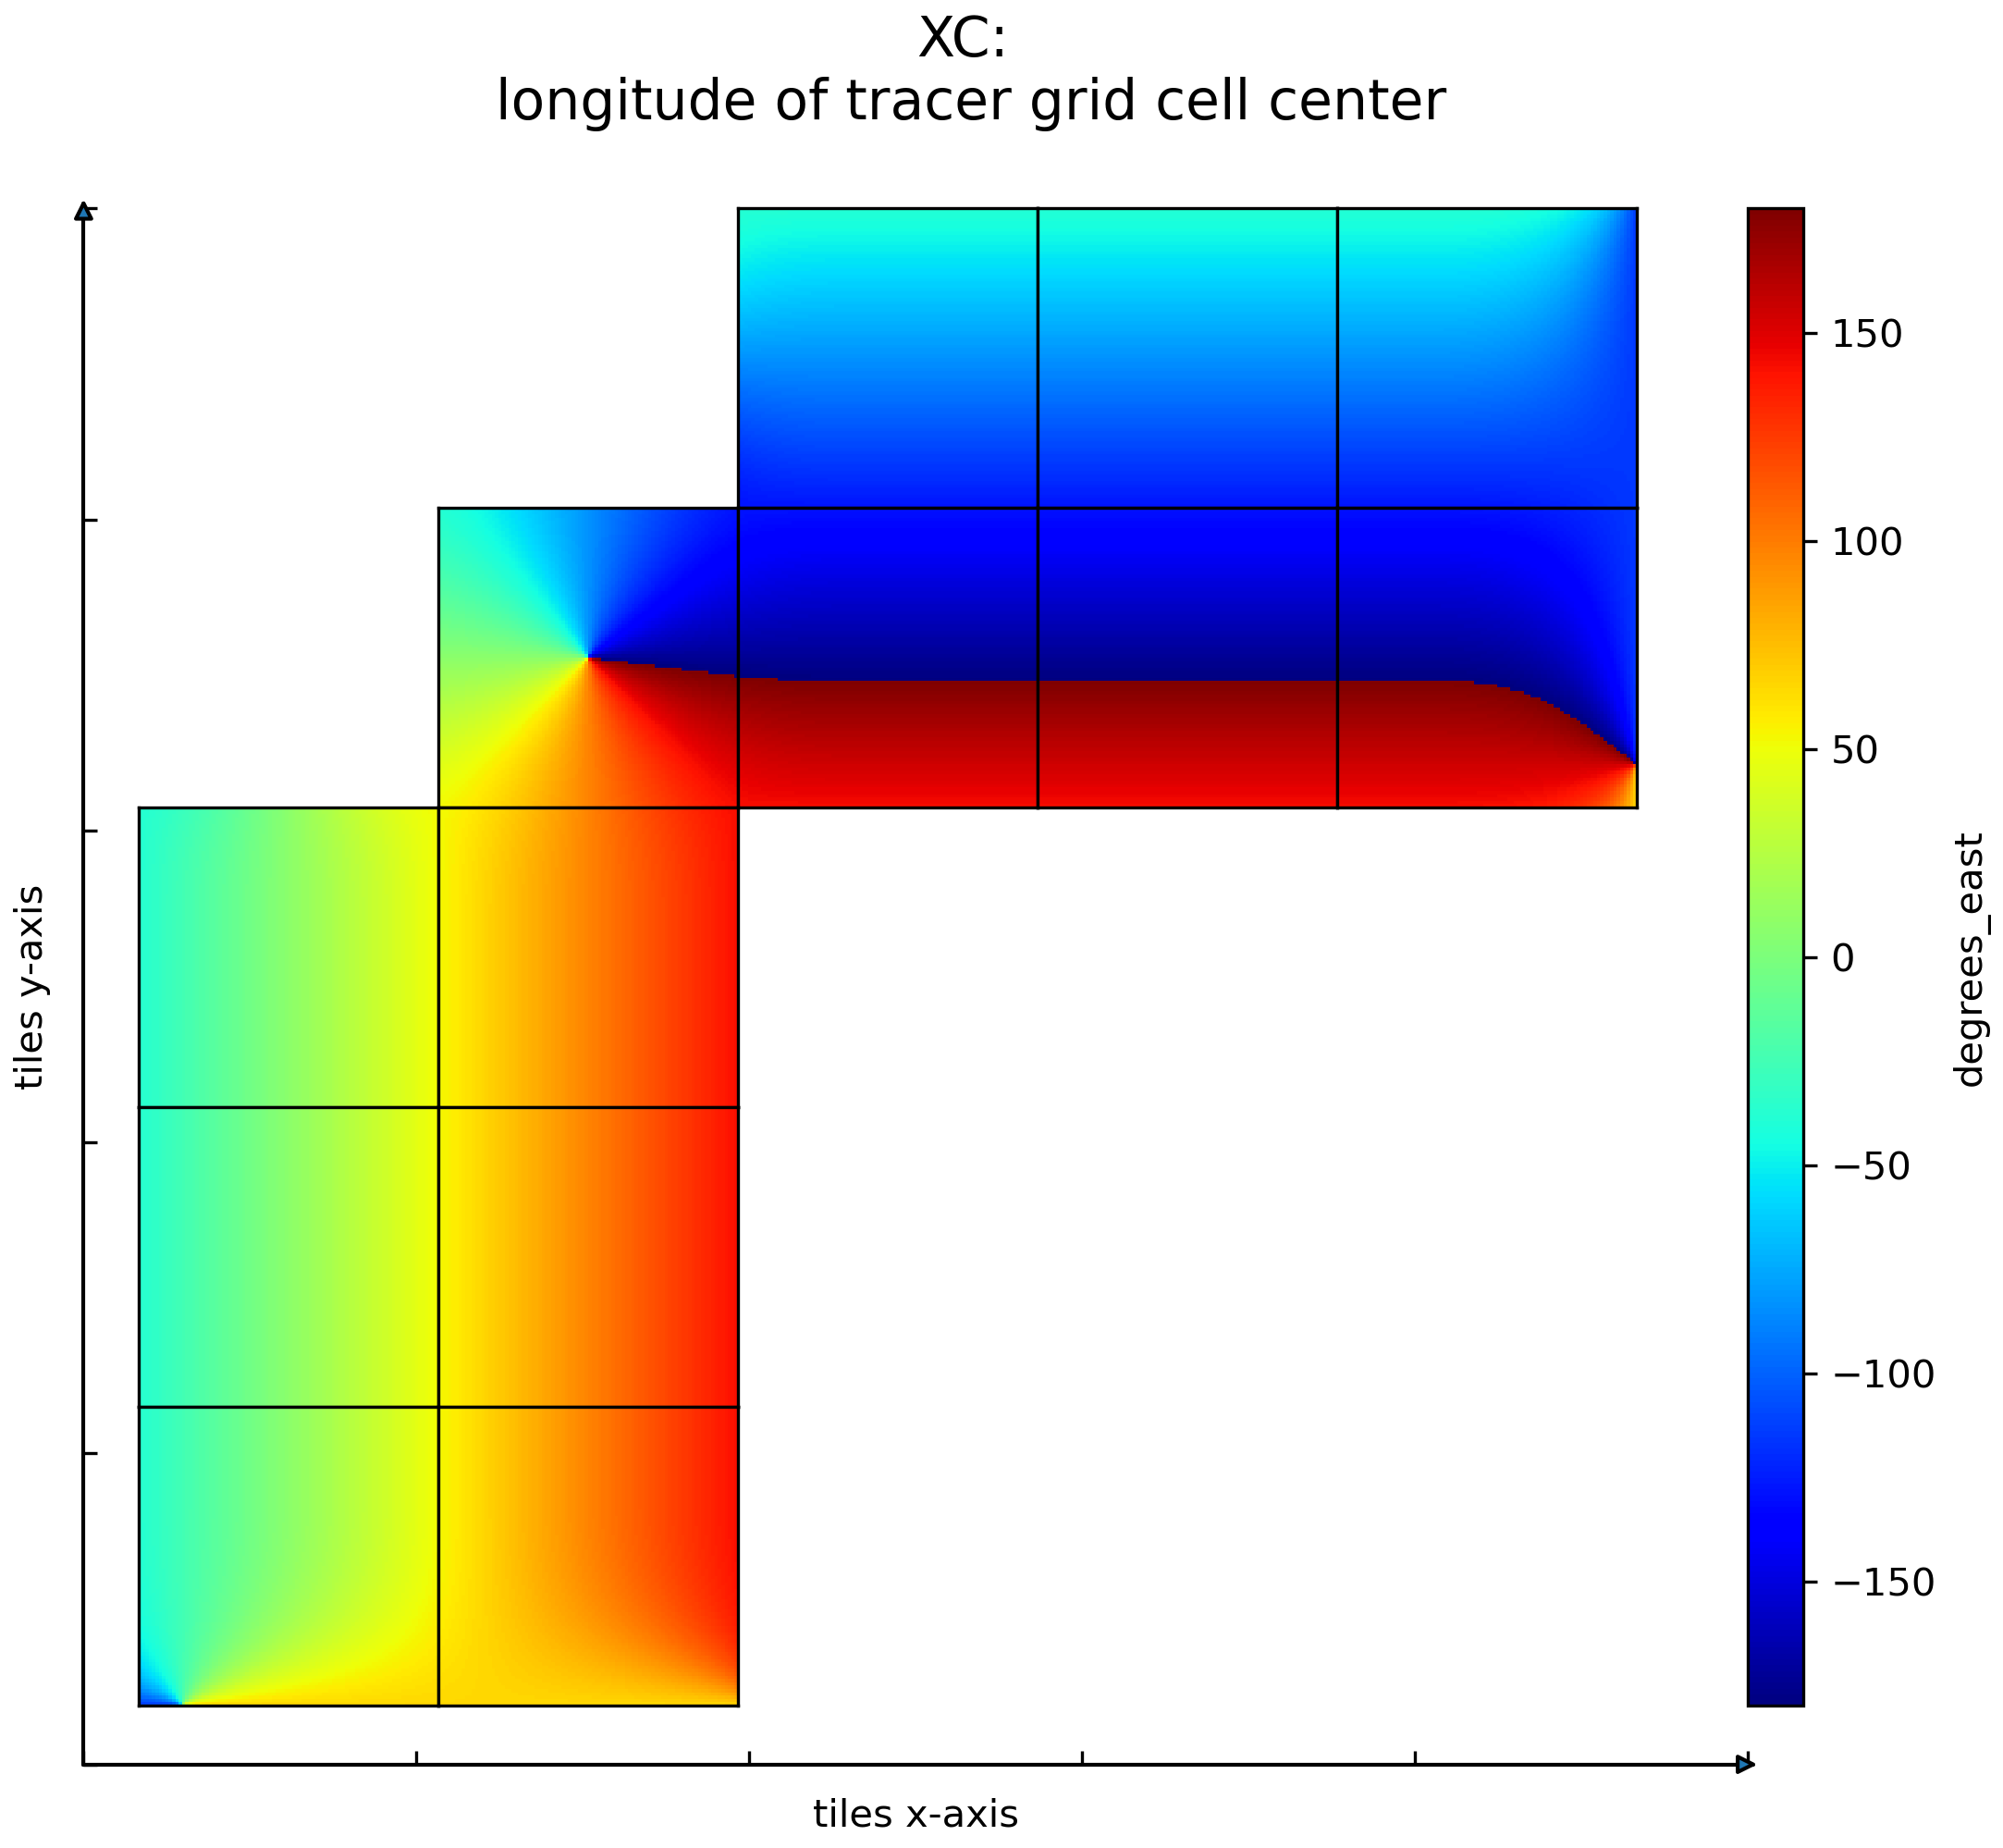
\includegraphics[scale=0.55]{../images/plots/native_plots_coords/Geometry_Parameters_for_the_Lat-Lon-Cap_90_(llc90)_Native_Model_Grid_(Version_4_Release_4)/XC.png}
\caption{Dataset: GRID\_GEOMETRY\_ECCO, Variable: XC}
\label{tab:table-GRID_GEOMETRY_ECCO_XC-Plot}
\end{figure}
\pagebreak
\subsubsection{Native coordinates Variable: YC}
\begin{longtable}{|m{0.06\textwidth}|m{0.3\textwidth}|m{0.45\textwidth}|m{0.11\textwidth}|}
\caption{Attributes description of the variable 'YC' from GRID\_GEOMETRY\_ECCO's  dataset.}
\label{tab:table-GRID_GEOMETRY_ECCO_YC} \\ 
\hline \endhead \hline \endfoot
\rowcolor{lightgray} \textbf{Storage Type} & \textbf{Variable Name} & \textbf{Description} & \textbf{Unit} \\ \hline
float32 & YC & Latitude of tracer grid cell center & degrees\_north \\ \hline
\multicolumn{4}{|c|}{\cellcolor{lightgray}{\textbf{Description of the variable in Common Data language (CDL)}}} \\ \hline
\multicolumn{4}{|c|}{\makecell{\parbox{.92\textwidth}{float32 YC(tile, j, i)\\
\hspace*{0.5cm}YC: long\_name = latitude of tracer grid cell center\\
\hspace*{0.5cm}YC: units = degrees\_north\\
\hspace*{0.5cm}YC: coordinate =\hspace*{0.5cm} YC XC\\
\hspace*{0.5cm}YC: bounds =\hspace*{0.5cm} YC\_bnds\\
\hspace*{0.5cm}YC: coverage\_content\_type = coordinate\\
\hspace*{0.5cm}YC: standard\_name = latitude}}} \\ \hline
\rowcolor{lightgray} \multicolumn{4}{|c|}{\textbf{Comments}} \\ \hline
\multicolumn{4}{|p{1\textwidth}|}{Nonuniform grid spacing} \\ \hline
\end{longtable}

\begin{figure}[H]
\centering
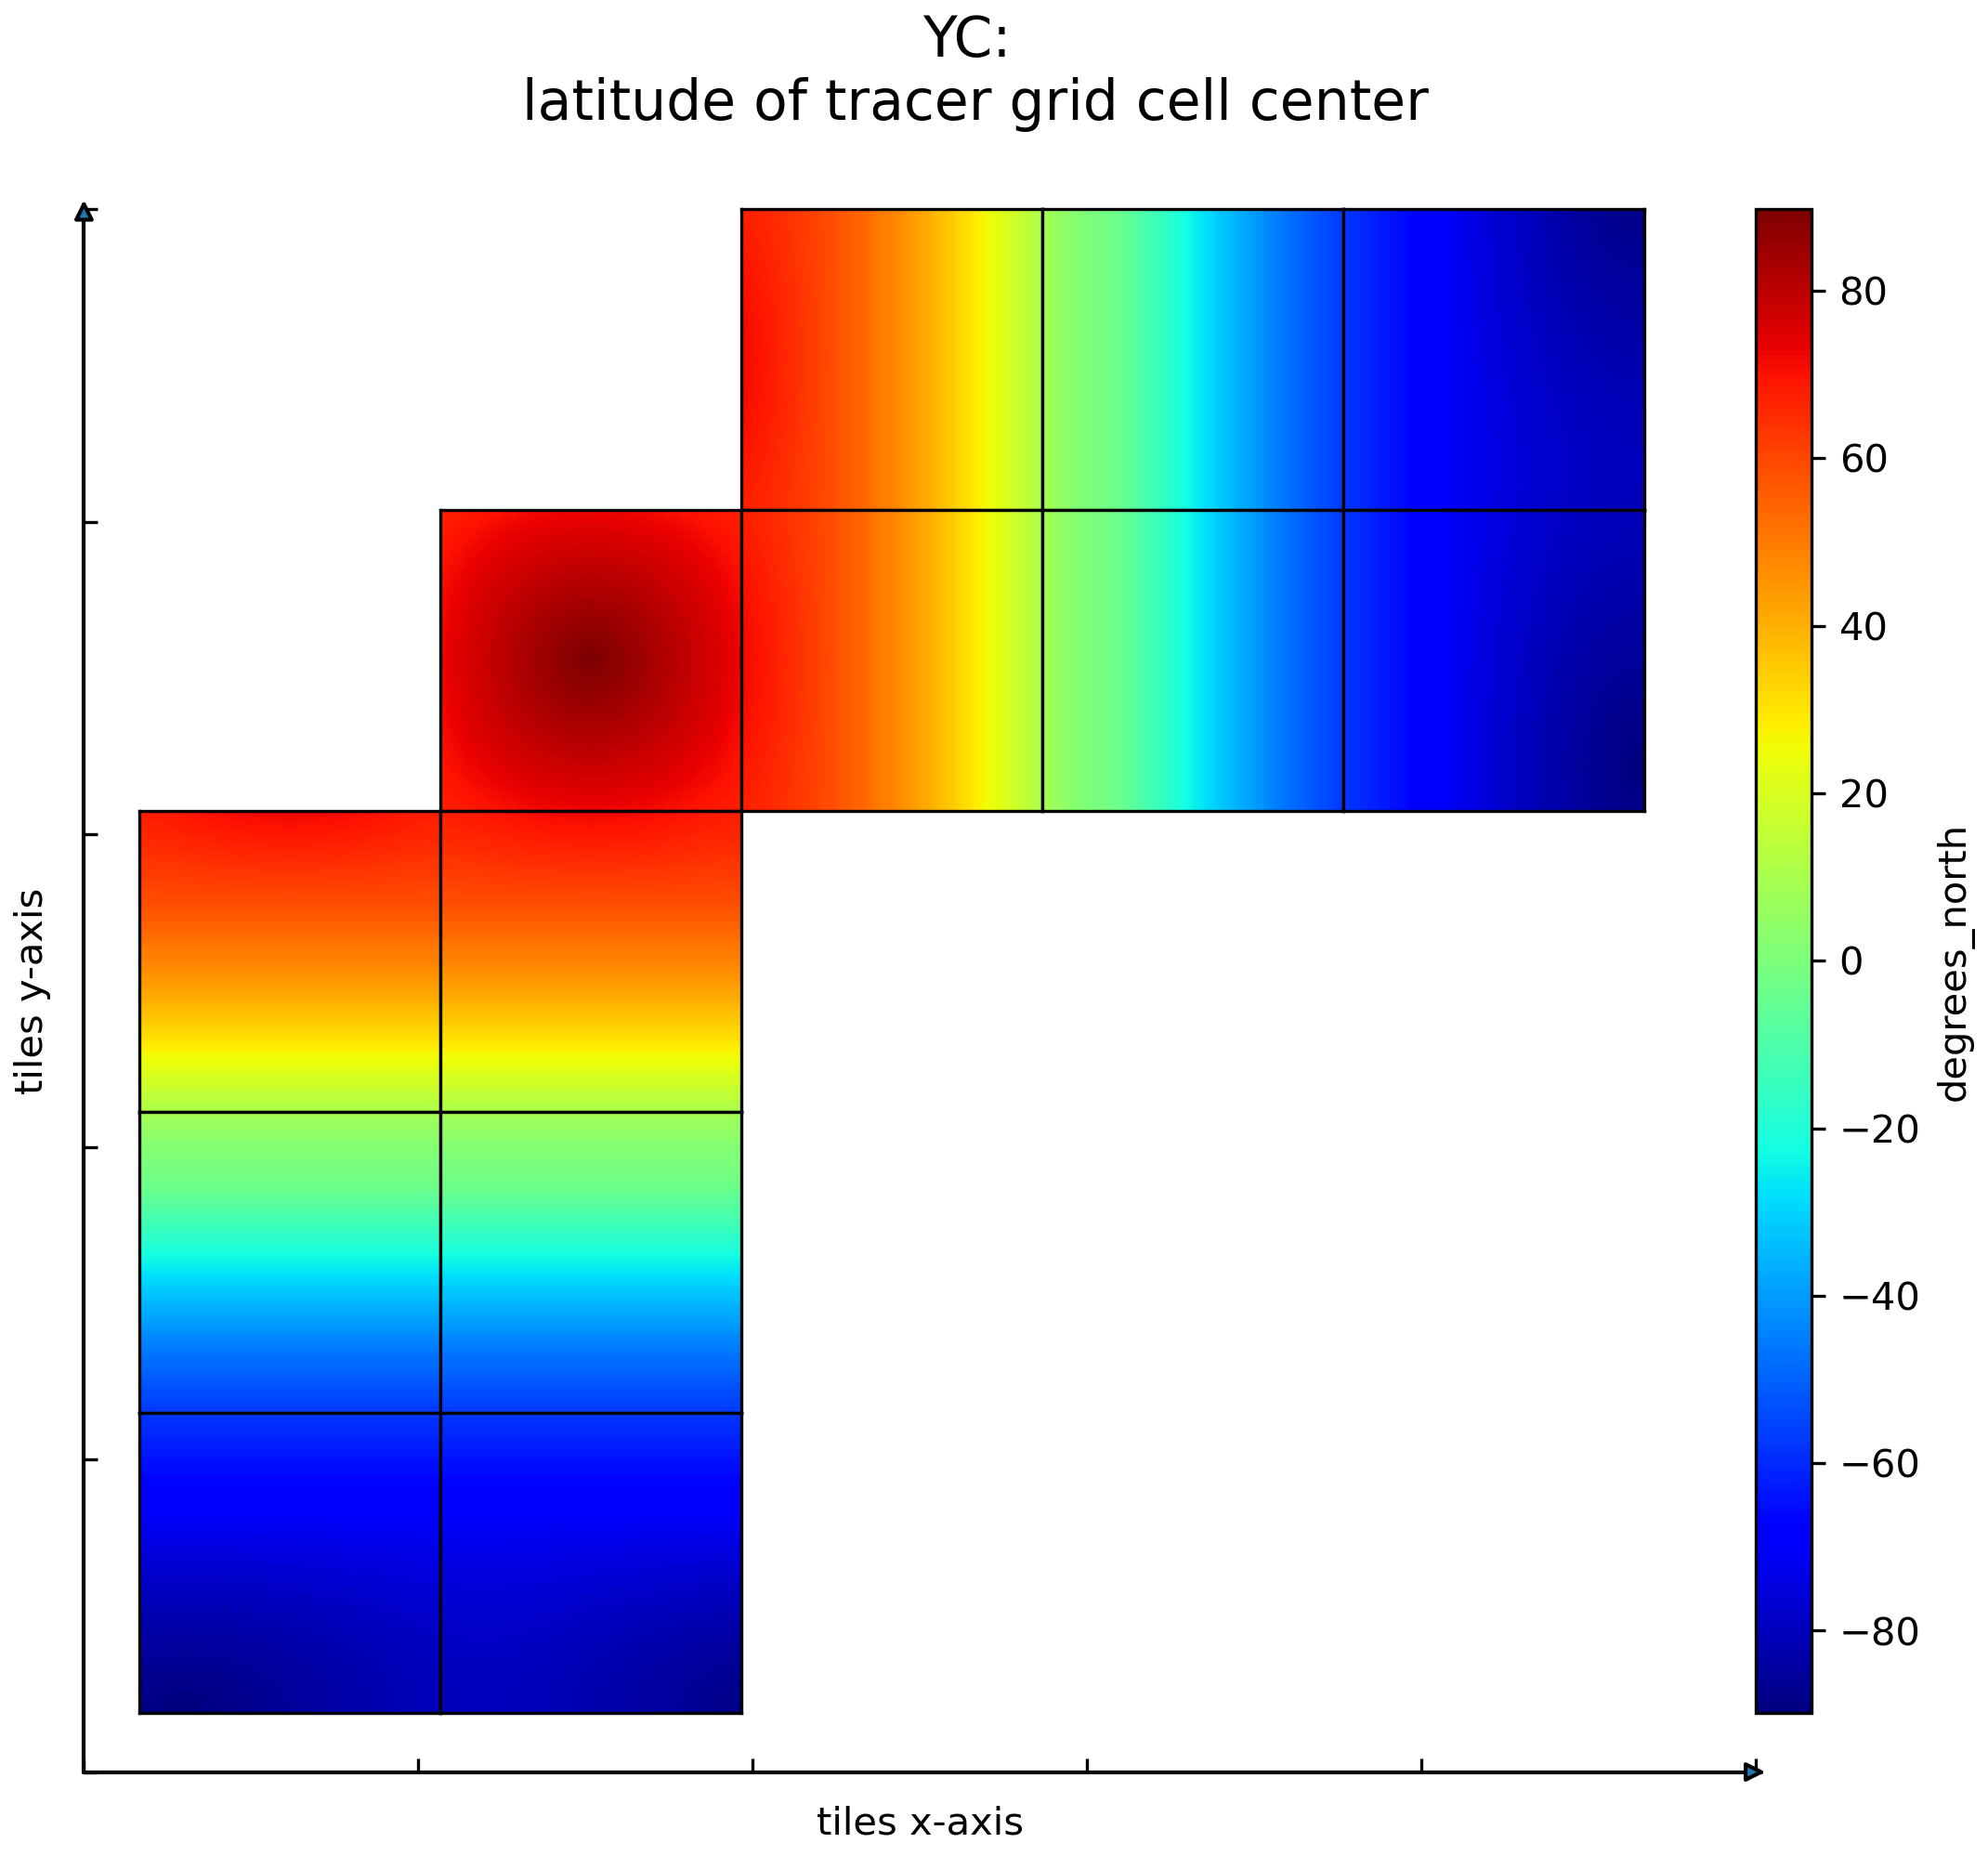
\includegraphics[scale=0.55]{../images/plots/native_plots_coords/Geometry_Parameters_for_the_Lat-Lon-Cap_90_(llc90)_Native_Model_Grid_(Version_4_Release_4)/YC.png}
\caption{Dataset: GRID\_GEOMETRY\_ECCO, Variable: YC}
\label{tab:table-GRID_GEOMETRY_ECCO_YC-Plot}
\end{figure}
\pagebreak
\subsubsection{Native coordinates Variable: XG}
\begin{longtable}{|m{0.06\textwidth}|m{0.3\textwidth}|m{0.45\textwidth}|m{0.11\textwidth}|}
\caption{Attributes description of the variable 'XG' from GRID\_GEOMETRY\_ECCO's  dataset.}
\label{tab:table-GRID_GEOMETRY_ECCO_XG} \\ 
\hline \endhead \hline \endfoot
\rowcolor{lightgray} \textbf{Storage Type} & \textbf{Variable Name} & \textbf{Description} & \textbf{Unit} \\ \hline
float32 & XG & Longitude of 'southwest' corner of tracer grid cell & degrees\_east \\ \hline
\multicolumn{4}{|c|}{\cellcolor{lightgray}{\textbf{Description of the variable in Common Data language (CDL)}}} \\ \hline
\multicolumn{4}{|c|}{\makecell{\parbox{.92\textwidth}{float32 XG(tile, j\_g, i\_g)\\
\hspace*{0.5cm}XG: long\_name = "longitude of southwest corner of tracer grid cell"\\
\hspace*{0.5cm}XG: units = degrees\_east\\
\hspace*{0.5cm}XG: coordinate = YG\hspace*{0.5cm} XG\\
\hspace*{0.5cm}XG: coverage\_content\_type = coordinate\\
\hspace*{0.5cm}XG: standard\_name = longitude}}} \\ \hline
\rowcolor{lightgray} \multicolumn{4}{|c|}{\textbf{Comments}} \\ \hline
\multicolumn{4}{|p{1\textwidth}|}{Nonuniform grid spacing. note: 'southwest' does not correspond to geographic orientation but is used for convenience to describe the computational grid. see mitgcm dcoumentation for details.} \\ \hline
\end{longtable}

\begin{figure}[H]
\centering
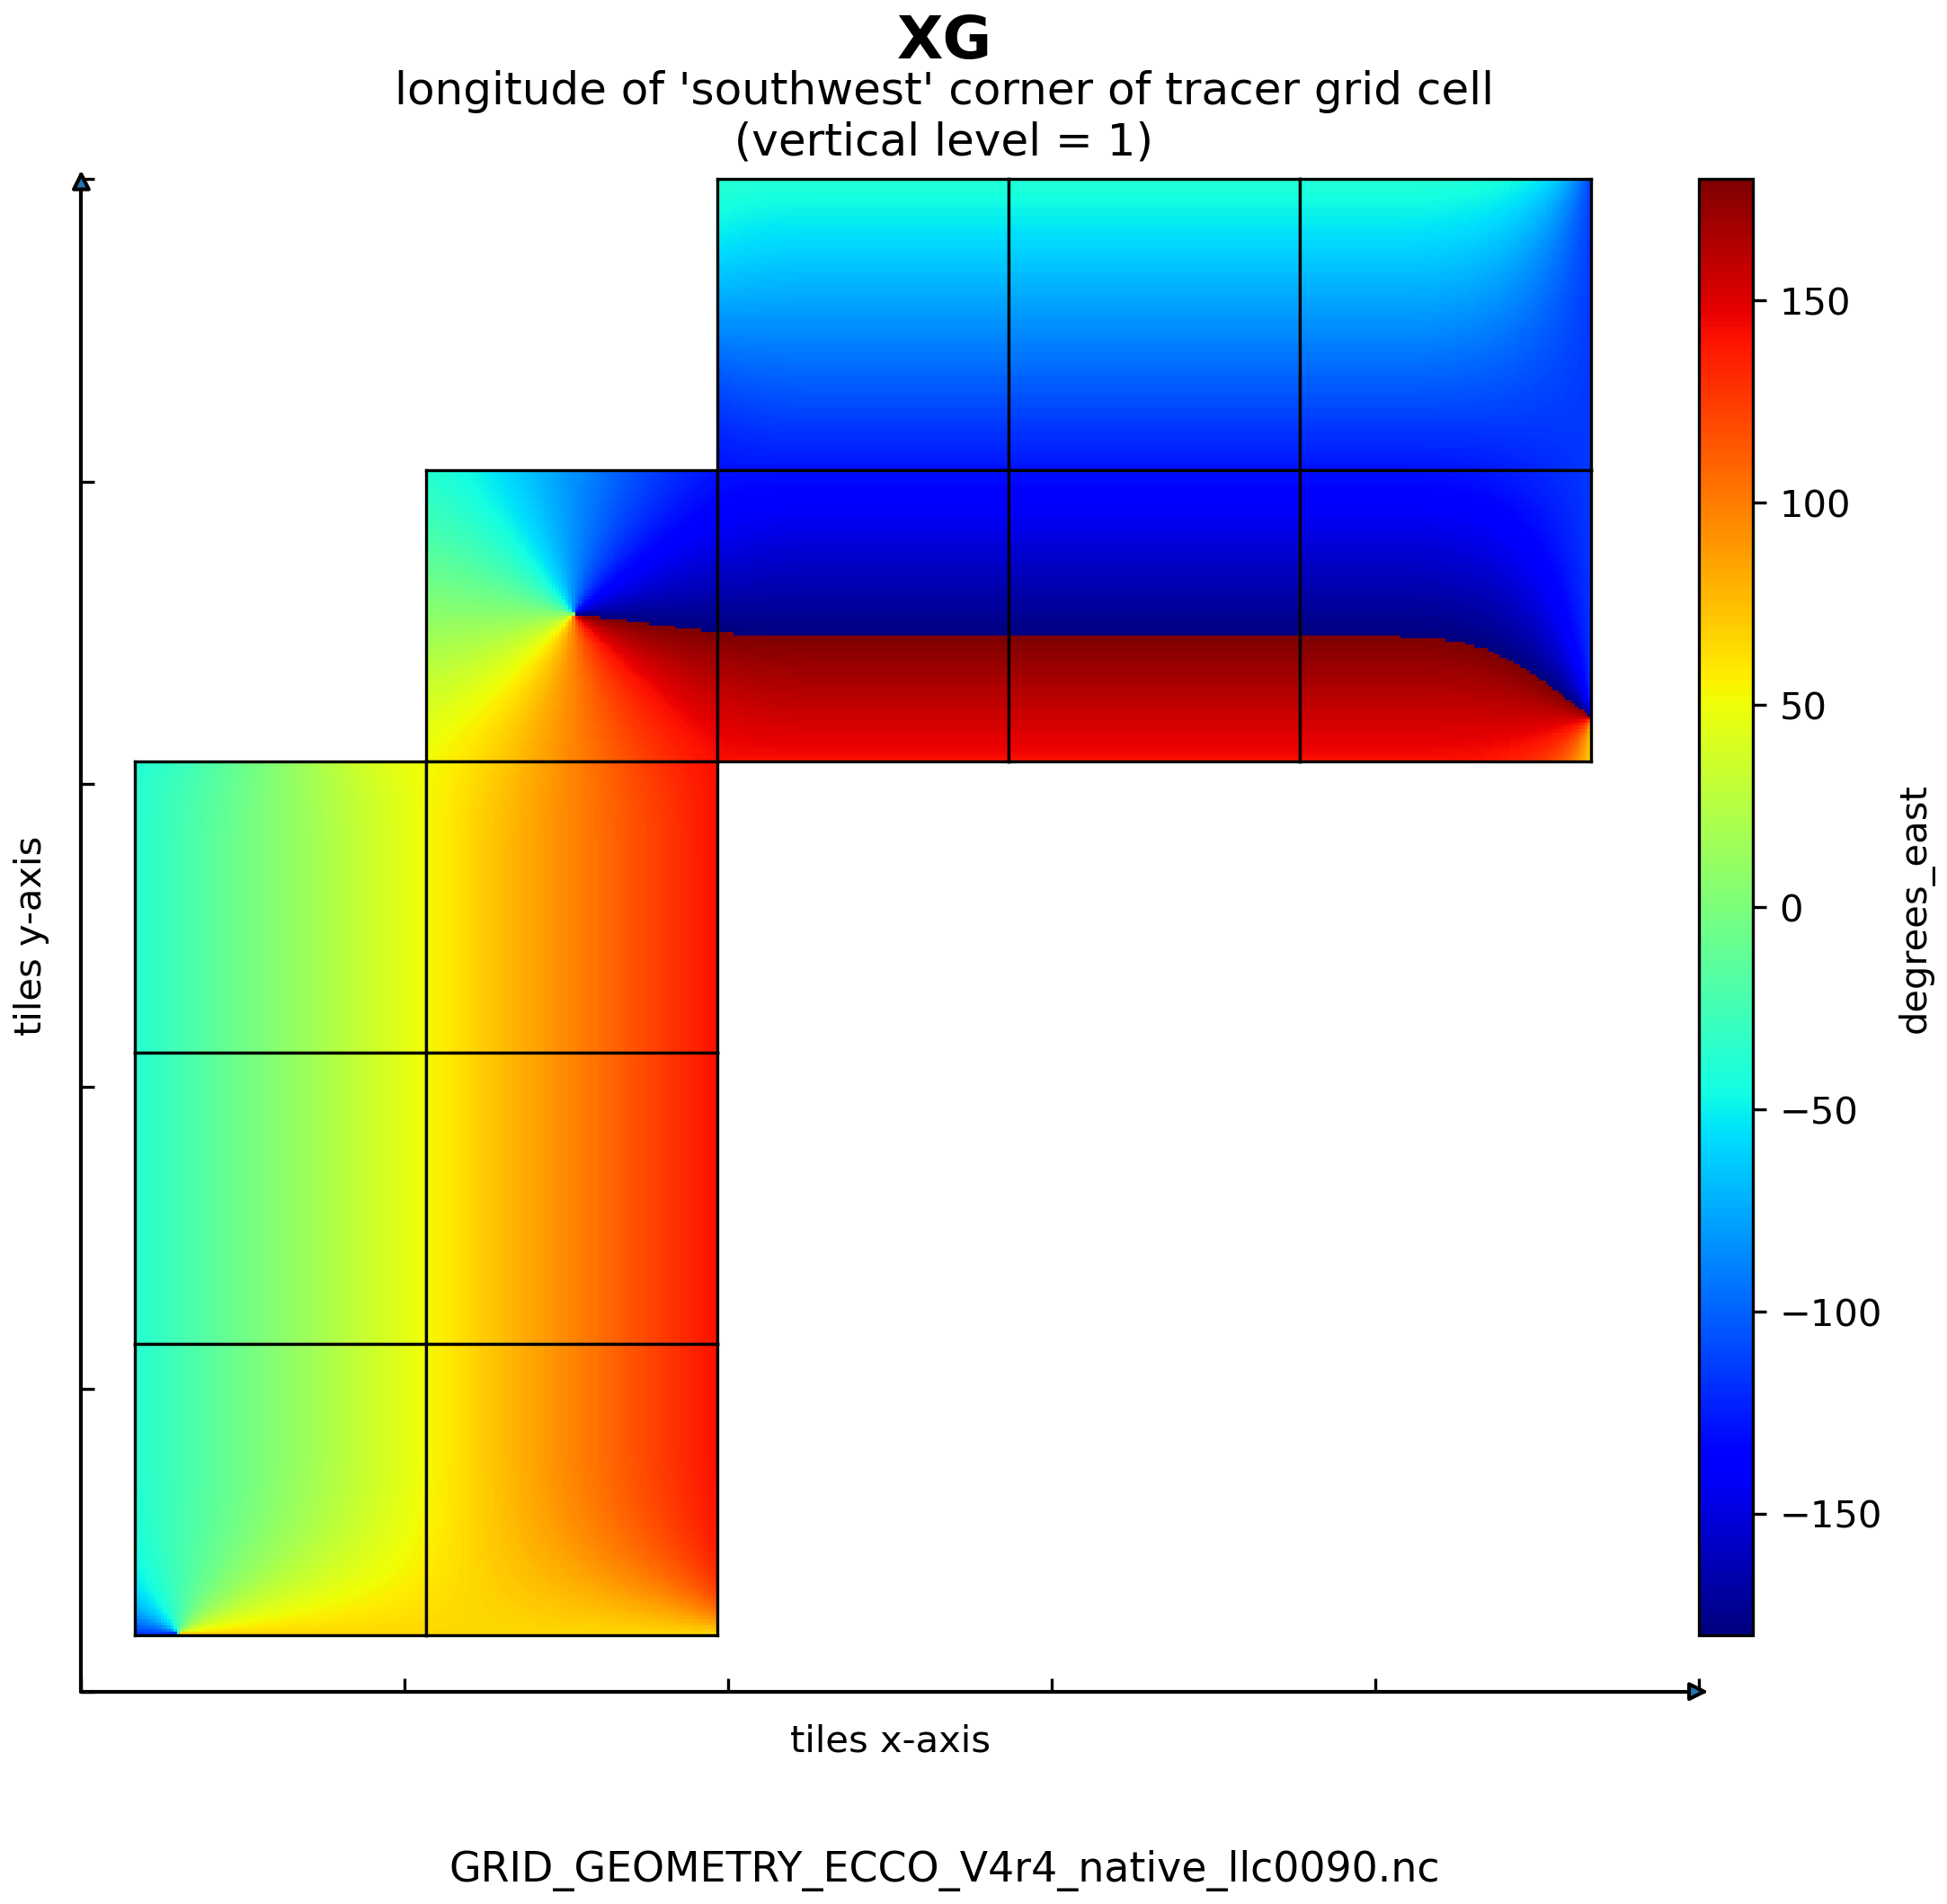
\includegraphics[scale=0.55]{../images/plots/native_plots_coords/Geometry_Parameters_for_the_Lat-Lon-Cap_90_(llc90)_Native_Model_Grid_(Version_4_Release_4)/XG.png}
\caption{Dataset: GRID\_GEOMETRY\_ECCO, Variable: XG}
\label{tab:table-GRID_GEOMETRY_ECCO_XG-Plot}
\end{figure}
\pagebreak
\subsubsection{Native coordinates Variable: YG}
\begin{longtable}{|m{0.06\textwidth}|m{0.3\textwidth}|m{0.45\textwidth}|m{0.11\textwidth}|}
\caption{Attributes description of the variable 'YG' from GRID\_GEOMETRY\_ECCO's  dataset.}
\label{tab:table-GRID_GEOMETRY_ECCO_YG} \\ 
\hline \endhead \hline \endfoot
\rowcolor{lightgray} \textbf{Storage Type} & \textbf{Variable Name} & \textbf{Description} & \textbf{Unit} \\ \hline
float32 & YG & Latitude of 'southwest' corner of tracer grid cell & degrees\_north \\ \hline
\multicolumn{4}{|c|}{\cellcolor{lightgray}{\textbf{Description of the variable in Common Data language (CDL)}}} \\ \hline
\multicolumn{4}{|c|}{\makecell{\parbox{.92\textwidth}{float32 YG(tile, j\_g, i\_g)\\
\hspace*{0.5cm}YG: long\_name = "latitude of southwest corner of tracer grid cell"\\
\hspace*{0.5cm}YG: units = degrees\_north\\
\hspace*{0.5cm}YG: coordinates =\hspace*{0.5cm} YG XG\\
\hspace*{0.5cm}YG: coverage\_content\_type = coordinate\\
\hspace*{0.5cm}YG: standard\_name = latitude}}} \\ \hline
\rowcolor{lightgray} \multicolumn{4}{|c|}{\textbf{Comments}} \\ \hline
\multicolumn{4}{|p{1\textwidth}|}{Nonuniform grid spacing. note: 'southwest' does not correspond to geographic orientation but is used for convenience to describe the computational grid. see mitgcm dcoumentation for details.} \\ \hline
\end{longtable}

\begin{figure}[H]
\centering
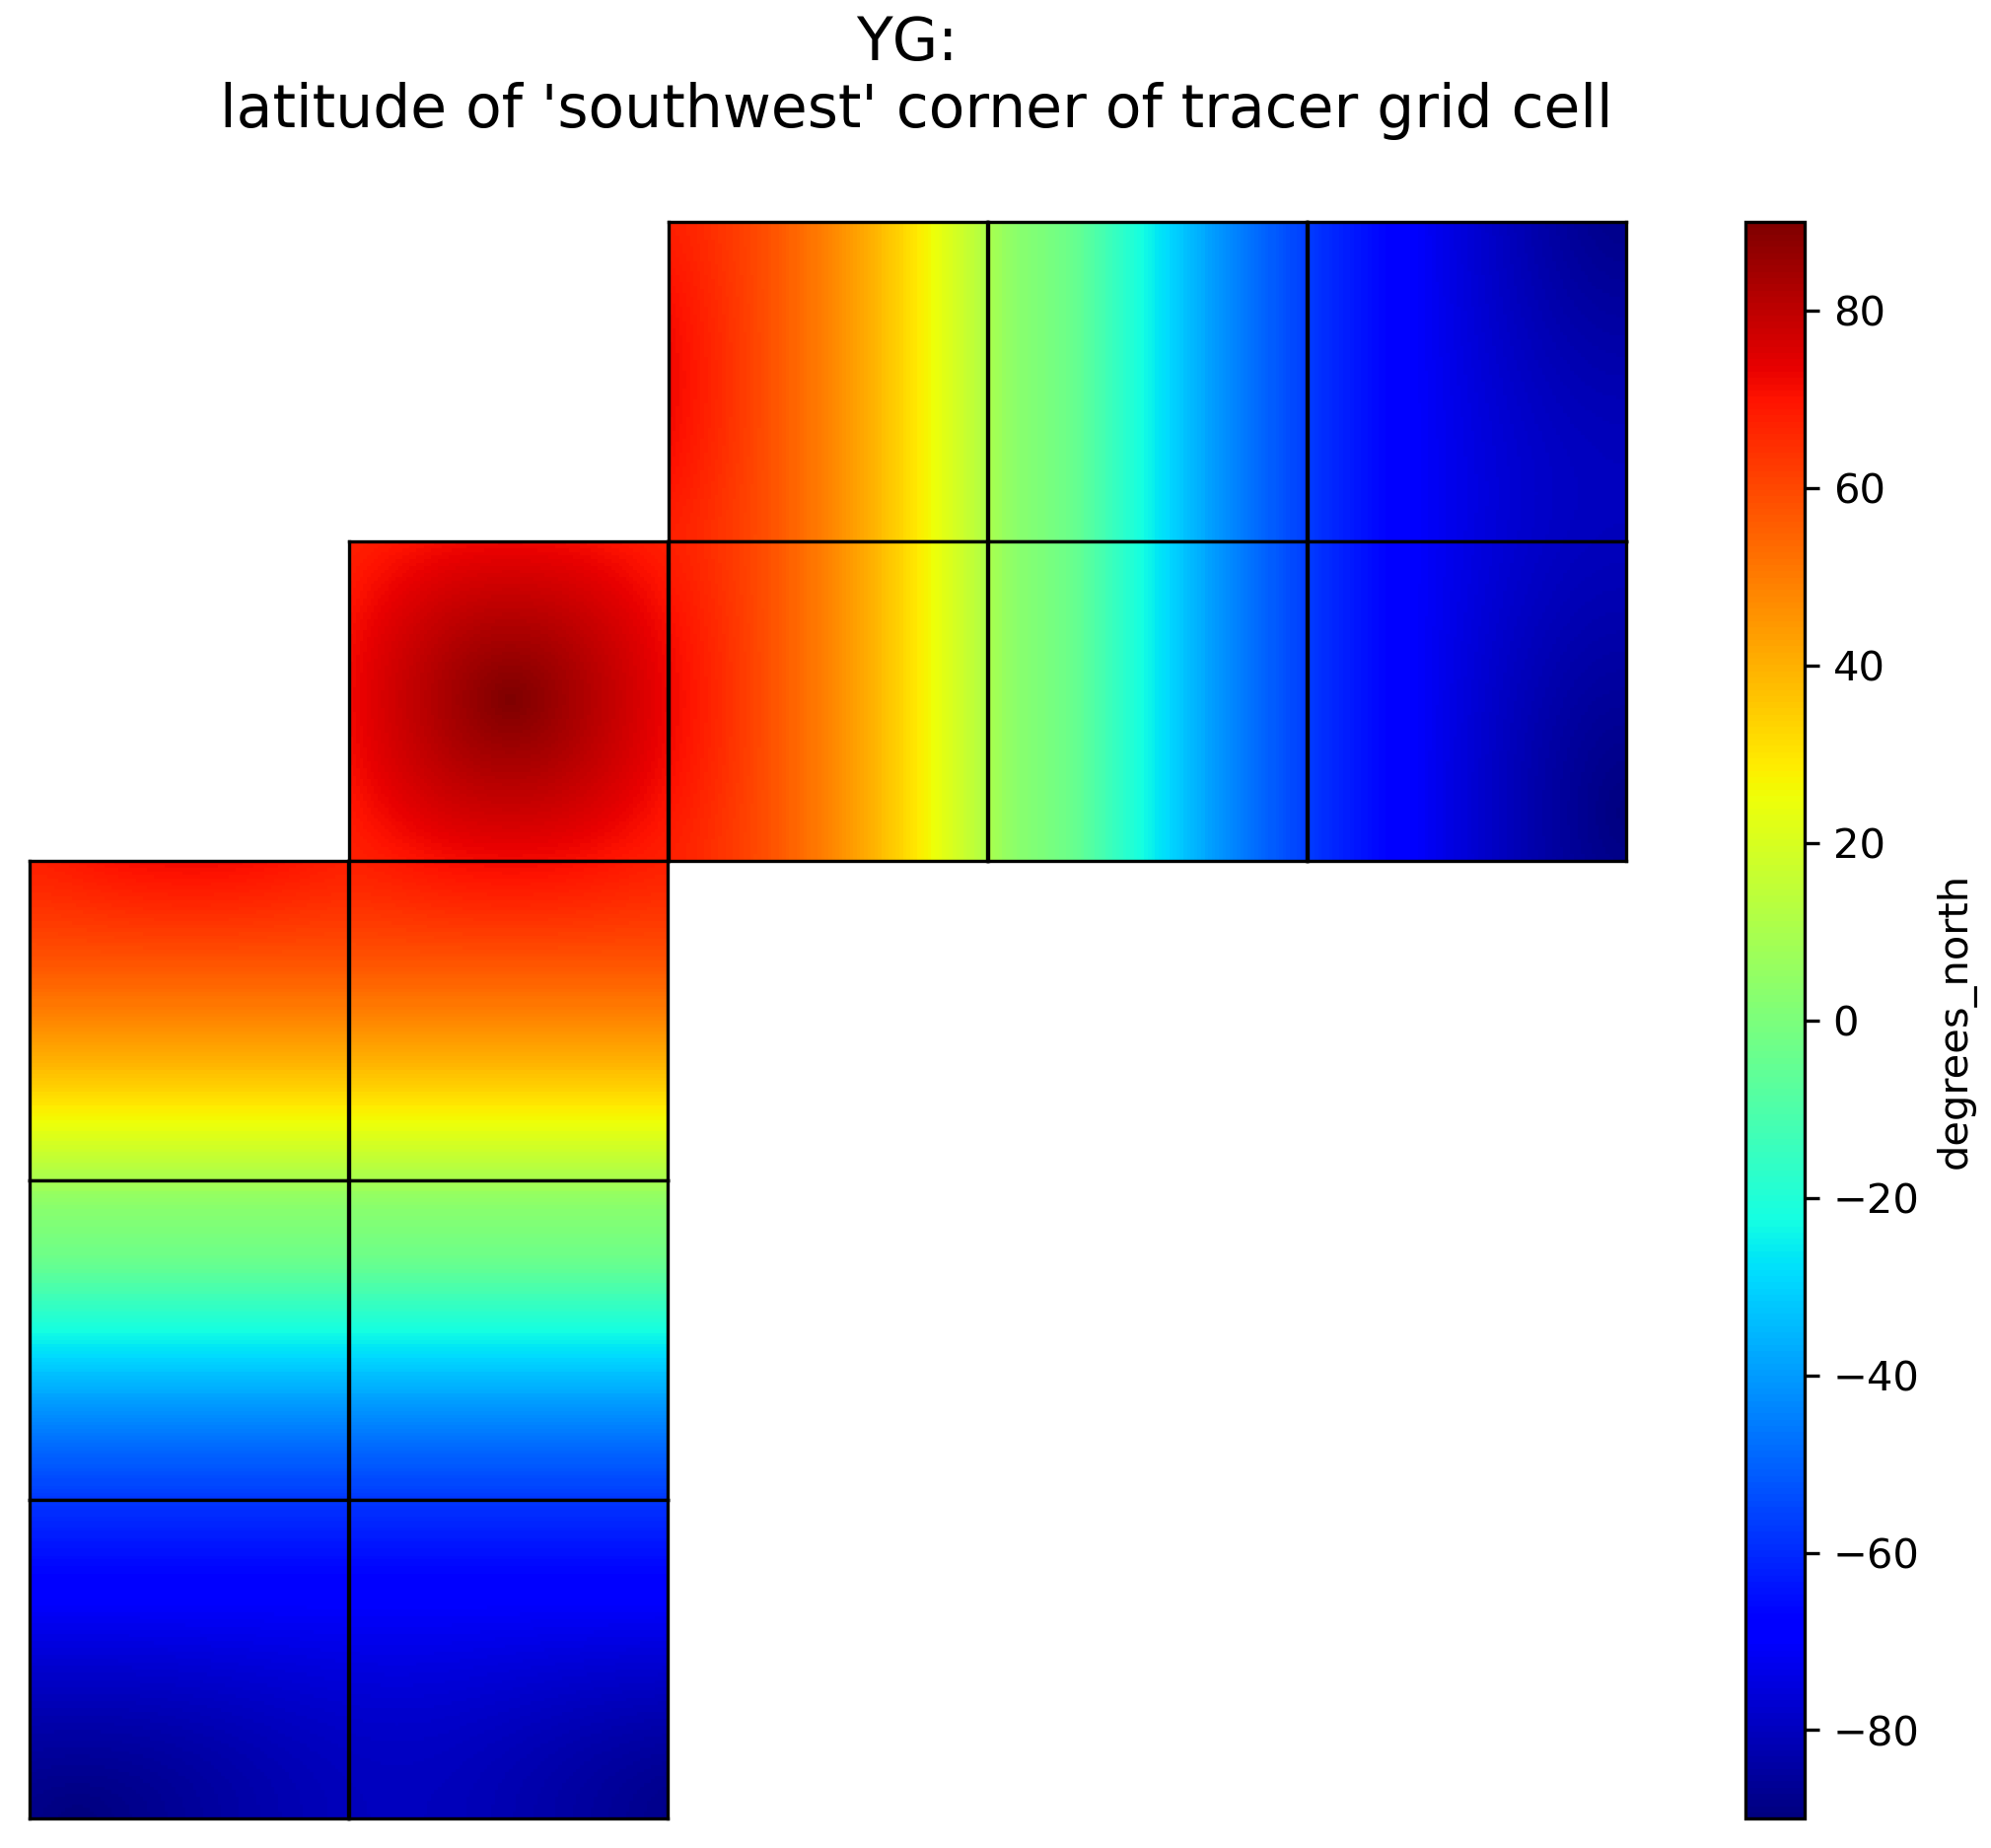
\includegraphics[scale=0.55]{../images/plots/native_plots_coords/Geometry_Parameters_for_the_Lat-Lon-Cap_90_(llc90)_Native_Model_Grid_(Version_4_Release_4)/YG.png}
\caption{Dataset: GRID\_GEOMETRY\_ECCO, Variable: YG}
\label{tab:table-GRID_GEOMETRY_ECCO_YG-Plot}
\end{figure}
\pagebreak
\subsubsection{Native coordinates Variable: CS}
\begin{longtable}{|m{0.06\textwidth}|m{0.3\textwidth}|m{0.45\textwidth}|m{0.11\textwidth}|}
\caption{Attributes description of the variable 'CS' from GRID\_GEOMETRY\_ECCO's  dataset.}
\label{tab:table-GRID_GEOMETRY_ECCO_CS} \\ 
\hline \endhead \hline \endfoot
\rowcolor{lightgray} \textbf{Storage Type} & \textbf{Variable Name} & \textbf{Description} & \textbf{Unit} \\ \hline
float32 & CS & Cosine of tracer grid cell orientation vs geographical north & 1 \\ \hline
\multicolumn{4}{|c|}{\cellcolor{lightgray}{\textbf{Description of the variable in Common Data language (CDL)}}} \\ \hline
\multicolumn{4}{|c|}{\makecell{\parbox{.92\textwidth}{float32 CS(tile, j, i)\\
\hspace*{0.5cm}CS: \_FillValue = 9.96921e+36\\
\hspace*{0.5cm}CS: long\_name = cosine of tracer grid cell orientation vs geographical north\\
\hspace*{0.5cm}CS: units = 1\\
\hspace*{0.5cm}CS: coordinate = YC XC\\
\hspace*{0.5cm}CS: coverage\_content\_type = modelResult\\
\hspace*{0.5cm}CS: coordinates = YC XC}}} \\ \hline
\rowcolor{lightgray} \multicolumn{4}{|c|}{\textbf{Comments}} \\ \hline
\multicolumn{4}{|p{1\textwidth}|}{Cs and sn are required to calculate the geographic (meridional, zonal) components of vectors on the curvilinear model grid. note: for vector r with components r\_x and r\_y: r\_\{east\} = cs r\_x - sn r\_y.  r\_\{north\} = sn r\_x + cs r\_y} \\ \hline
\end{longtable}

\begin{figure}[H]
\centering
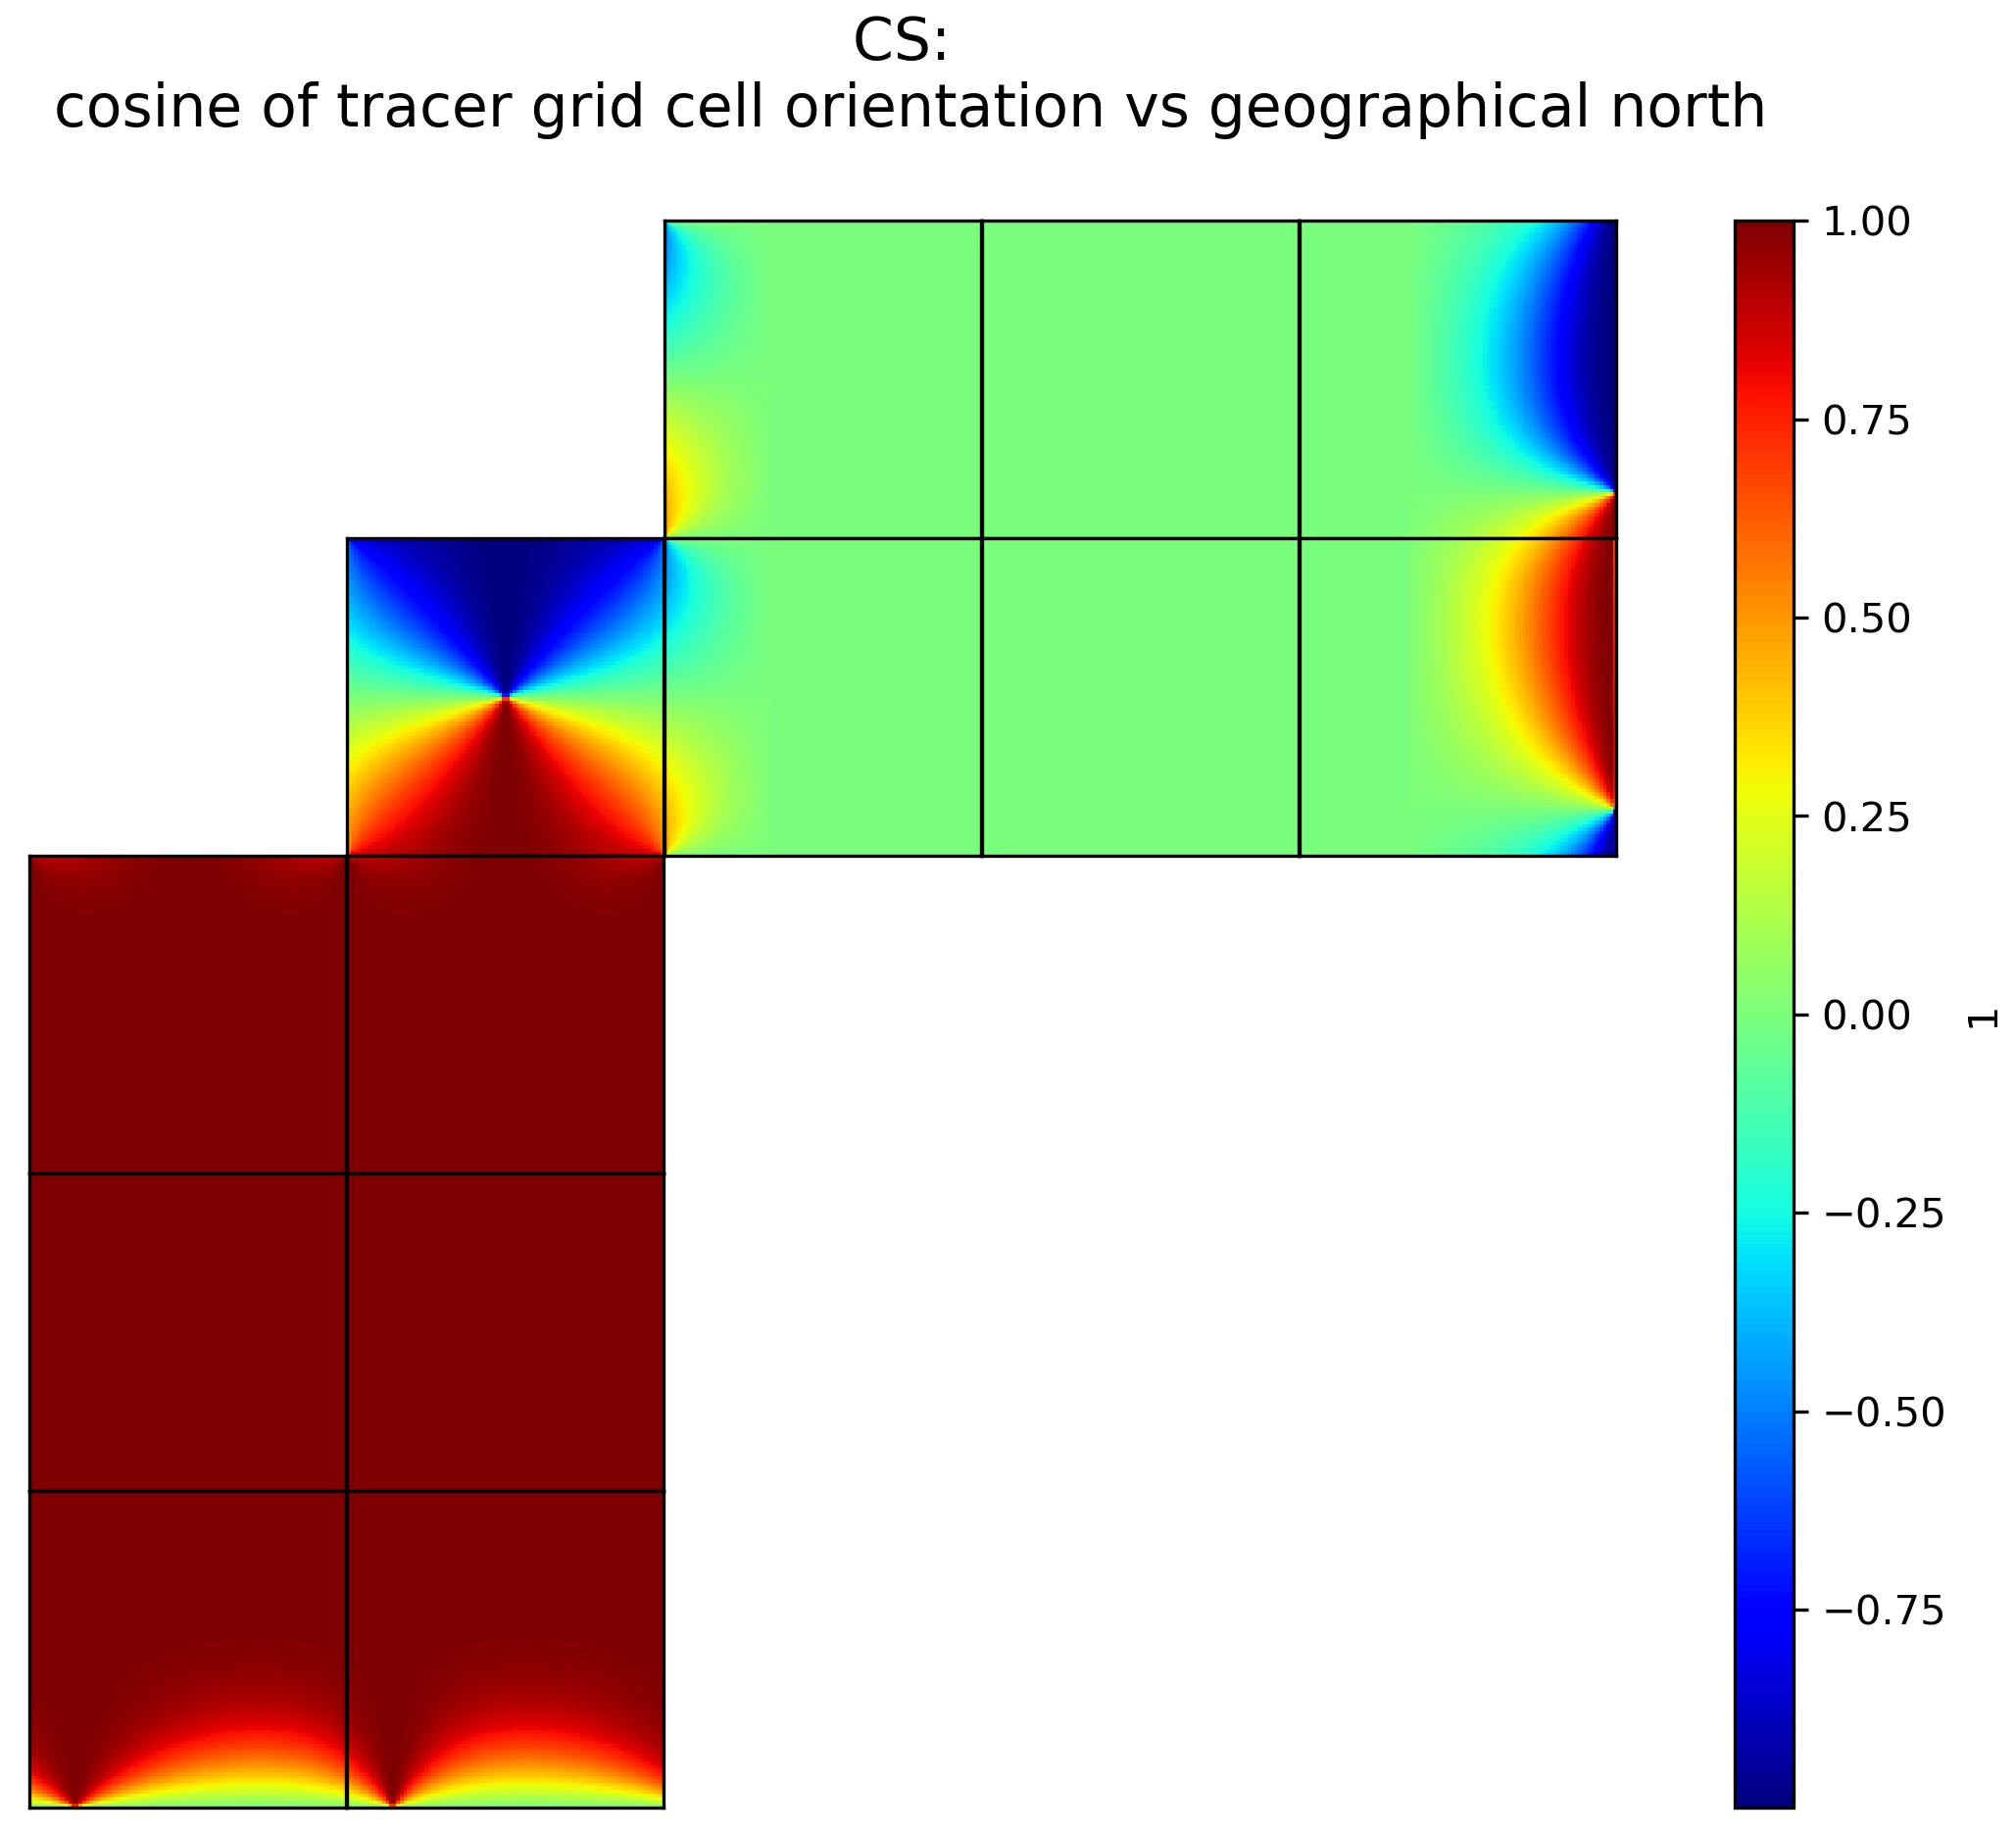
\includegraphics[scale=0.55]{../images/plots/native_plots_coords/Geometry_Parameters_for_the_Lat-Lon-Cap_90_(llc90)_Native_Model_Grid_(Version_4_Release_4)/CS.png}
\caption{Dataset: GRID\_GEOMETRY\_ECCO, Variable: CS}
\label{tab:table-GRID_GEOMETRY_ECCO_CS-Plot}
\end{figure}
\pagebreak
\subsubsection{Native coordinates Variable: SN}
\begin{longtable}{|m{0.06\textwidth}|m{0.3\textwidth}|m{0.45\textwidth}|m{0.11\textwidth}|}
\caption{Attributes description of the variable 'SN' from GRID\_GEOMETRY\_ECCO's  dataset.}
\label{tab:table-GRID_GEOMETRY_ECCO_SN} \\ 
\hline \endhead \hline \endfoot
\rowcolor{lightgray} \textbf{Storage Type} & \textbf{Variable Name} & \textbf{Description} & \textbf{Unit} \\ \hline
float32 & SN & Sine of tracer grid cell orientation vs geographical north & 1 \\ \hline
\multicolumn{4}{|c|}{\cellcolor{lightgray}{\textbf{Description of the variable in Common Data language (CDL)}}} \\ \hline
\multicolumn{4}{|c|}{\makecell{\parbox{.92\textwidth}{float32 SN(tile, j, i)\\
\hspace*{0.5cm}SN: \_FillValue = 9.96921e+36\\
\hspace*{0.5cm}SN: long\_name = sine of tracer grid cell orientation vs geographical north\\
\hspace*{0.5cm}SN: units = 1\\
\hspace*{0.5cm}SN: coordinate = YC XC\\
\hspace*{0.5cm}SN: coverage\_content\_type = modelResult\\
\hspace*{0.5cm}SN: coordinates = YC XC}}} \\ \hline
\rowcolor{lightgray} \multicolumn{4}{|c|}{\textbf{Comments}} \\ \hline
\multicolumn{4}{|p{1\textwidth}|}{Cs and sn are required to calculate the geographic (meridional, zonal) components of vectors on the curvilinear model grid. note: for vector r with components r\_x and r\_y in local grid directions x and y, the geographical eastward component r\_\{east\} = cs r\_x - sn r\_y. the geographical northward component r\_\{north\} = sn r\_x + cs r\_y.} \\ \hline
\end{longtable}

\begin{figure}[H]
\centering
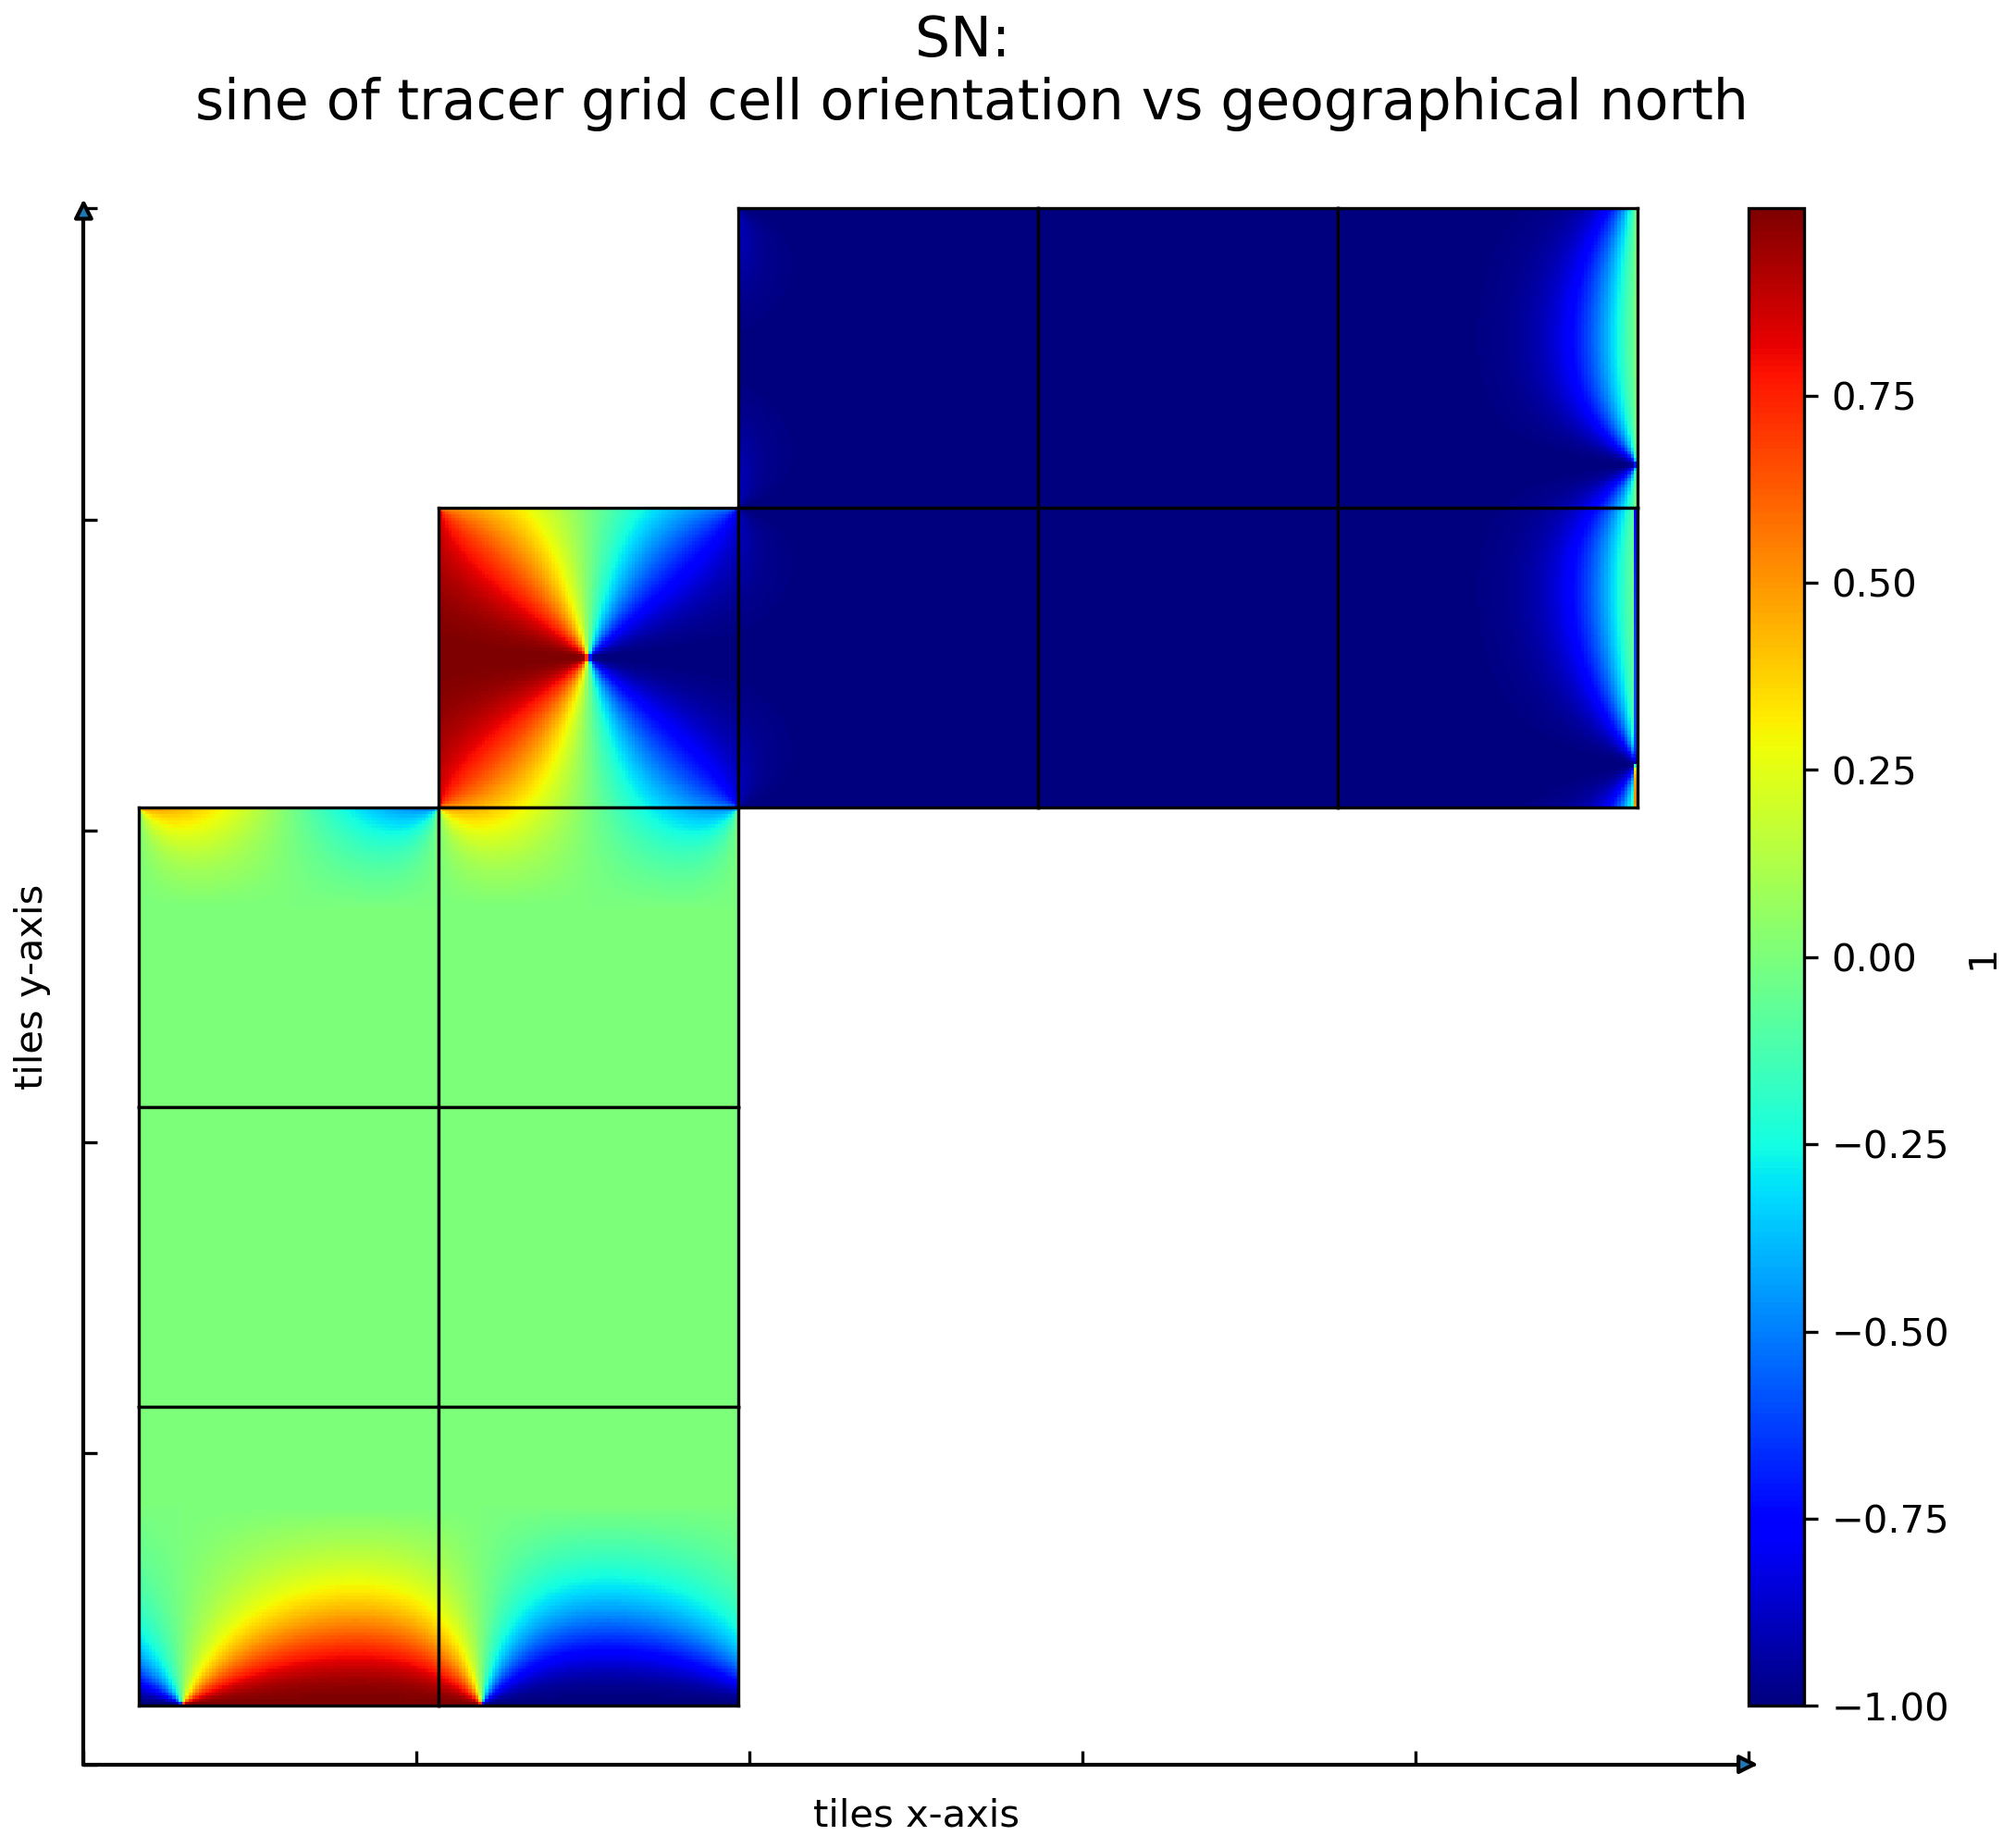
\includegraphics[scale=0.55]{../images/plots/native_plots_coords/Geometry_Parameters_for_the_Lat-Lon-Cap_90_(llc90)_Native_Model_Grid_(Version_4_Release_4)/SN.png}
\caption{Dataset: GRID\_GEOMETRY\_ECCO, Variable: SN}
\label{tab:table-GRID_GEOMETRY_ECCO_SN-Plot}
\end{figure}
\pagebreak
\subsubsection{Native coordinates Variable: rA}
\begin{longtable}{|m{0.06\textwidth}|m{0.3\textwidth}|m{0.45\textwidth}|m{0.11\textwidth}|}
\caption{Attributes description of the variable 'rA' from GRID\_GEOMETRY\_ECCO's  dataset.}
\label{tab:table-GRID_GEOMETRY_ECCO_rA} \\ 
\hline \endhead \hline \endfoot
\rowcolor{lightgray} \textbf{Storage Type} & \textbf{Variable Name} & \textbf{Description} & \textbf{Unit} \\ \hline
float32 & rA & Area of tracer grid cell & m2 \\ \hline
\multicolumn{4}{|c|}{\cellcolor{lightgray}{\textbf{Description of the variable in Common Data language (CDL)}}} \\ \hline
\multicolumn{4}{|c|}{\makecell{\parbox{.92\textwidth}{float32 rA(tile, j, i)\\
\hspace*{0.5cm}rA: \_FillValue = 9.96921e+36\\
\hspace*{0.5cm}rA: long\_name = area of tracer grid cell\\
\hspace*{0.5cm}rA: units = m2\\
\hspace*{0.5cm}rA: coordinate = YC XC\\
\hspace*{0.5cm}rA: coverage\_content\_type = modelResult\\
\hspace*{0.5cm}rA: standard\_name = cell\_area\\
\hspace*{0.5cm}rA: coordinates = YC XC}}} \\ \hline
\rowcolor{lightgray} \multicolumn{4}{|c|}{\textbf{Comments}} \\ \hline
\multicolumn{4}{|p{1\textwidth}|}{N/a} \\ \hline
\end{longtable}

\begin{figure}[H]
\centering
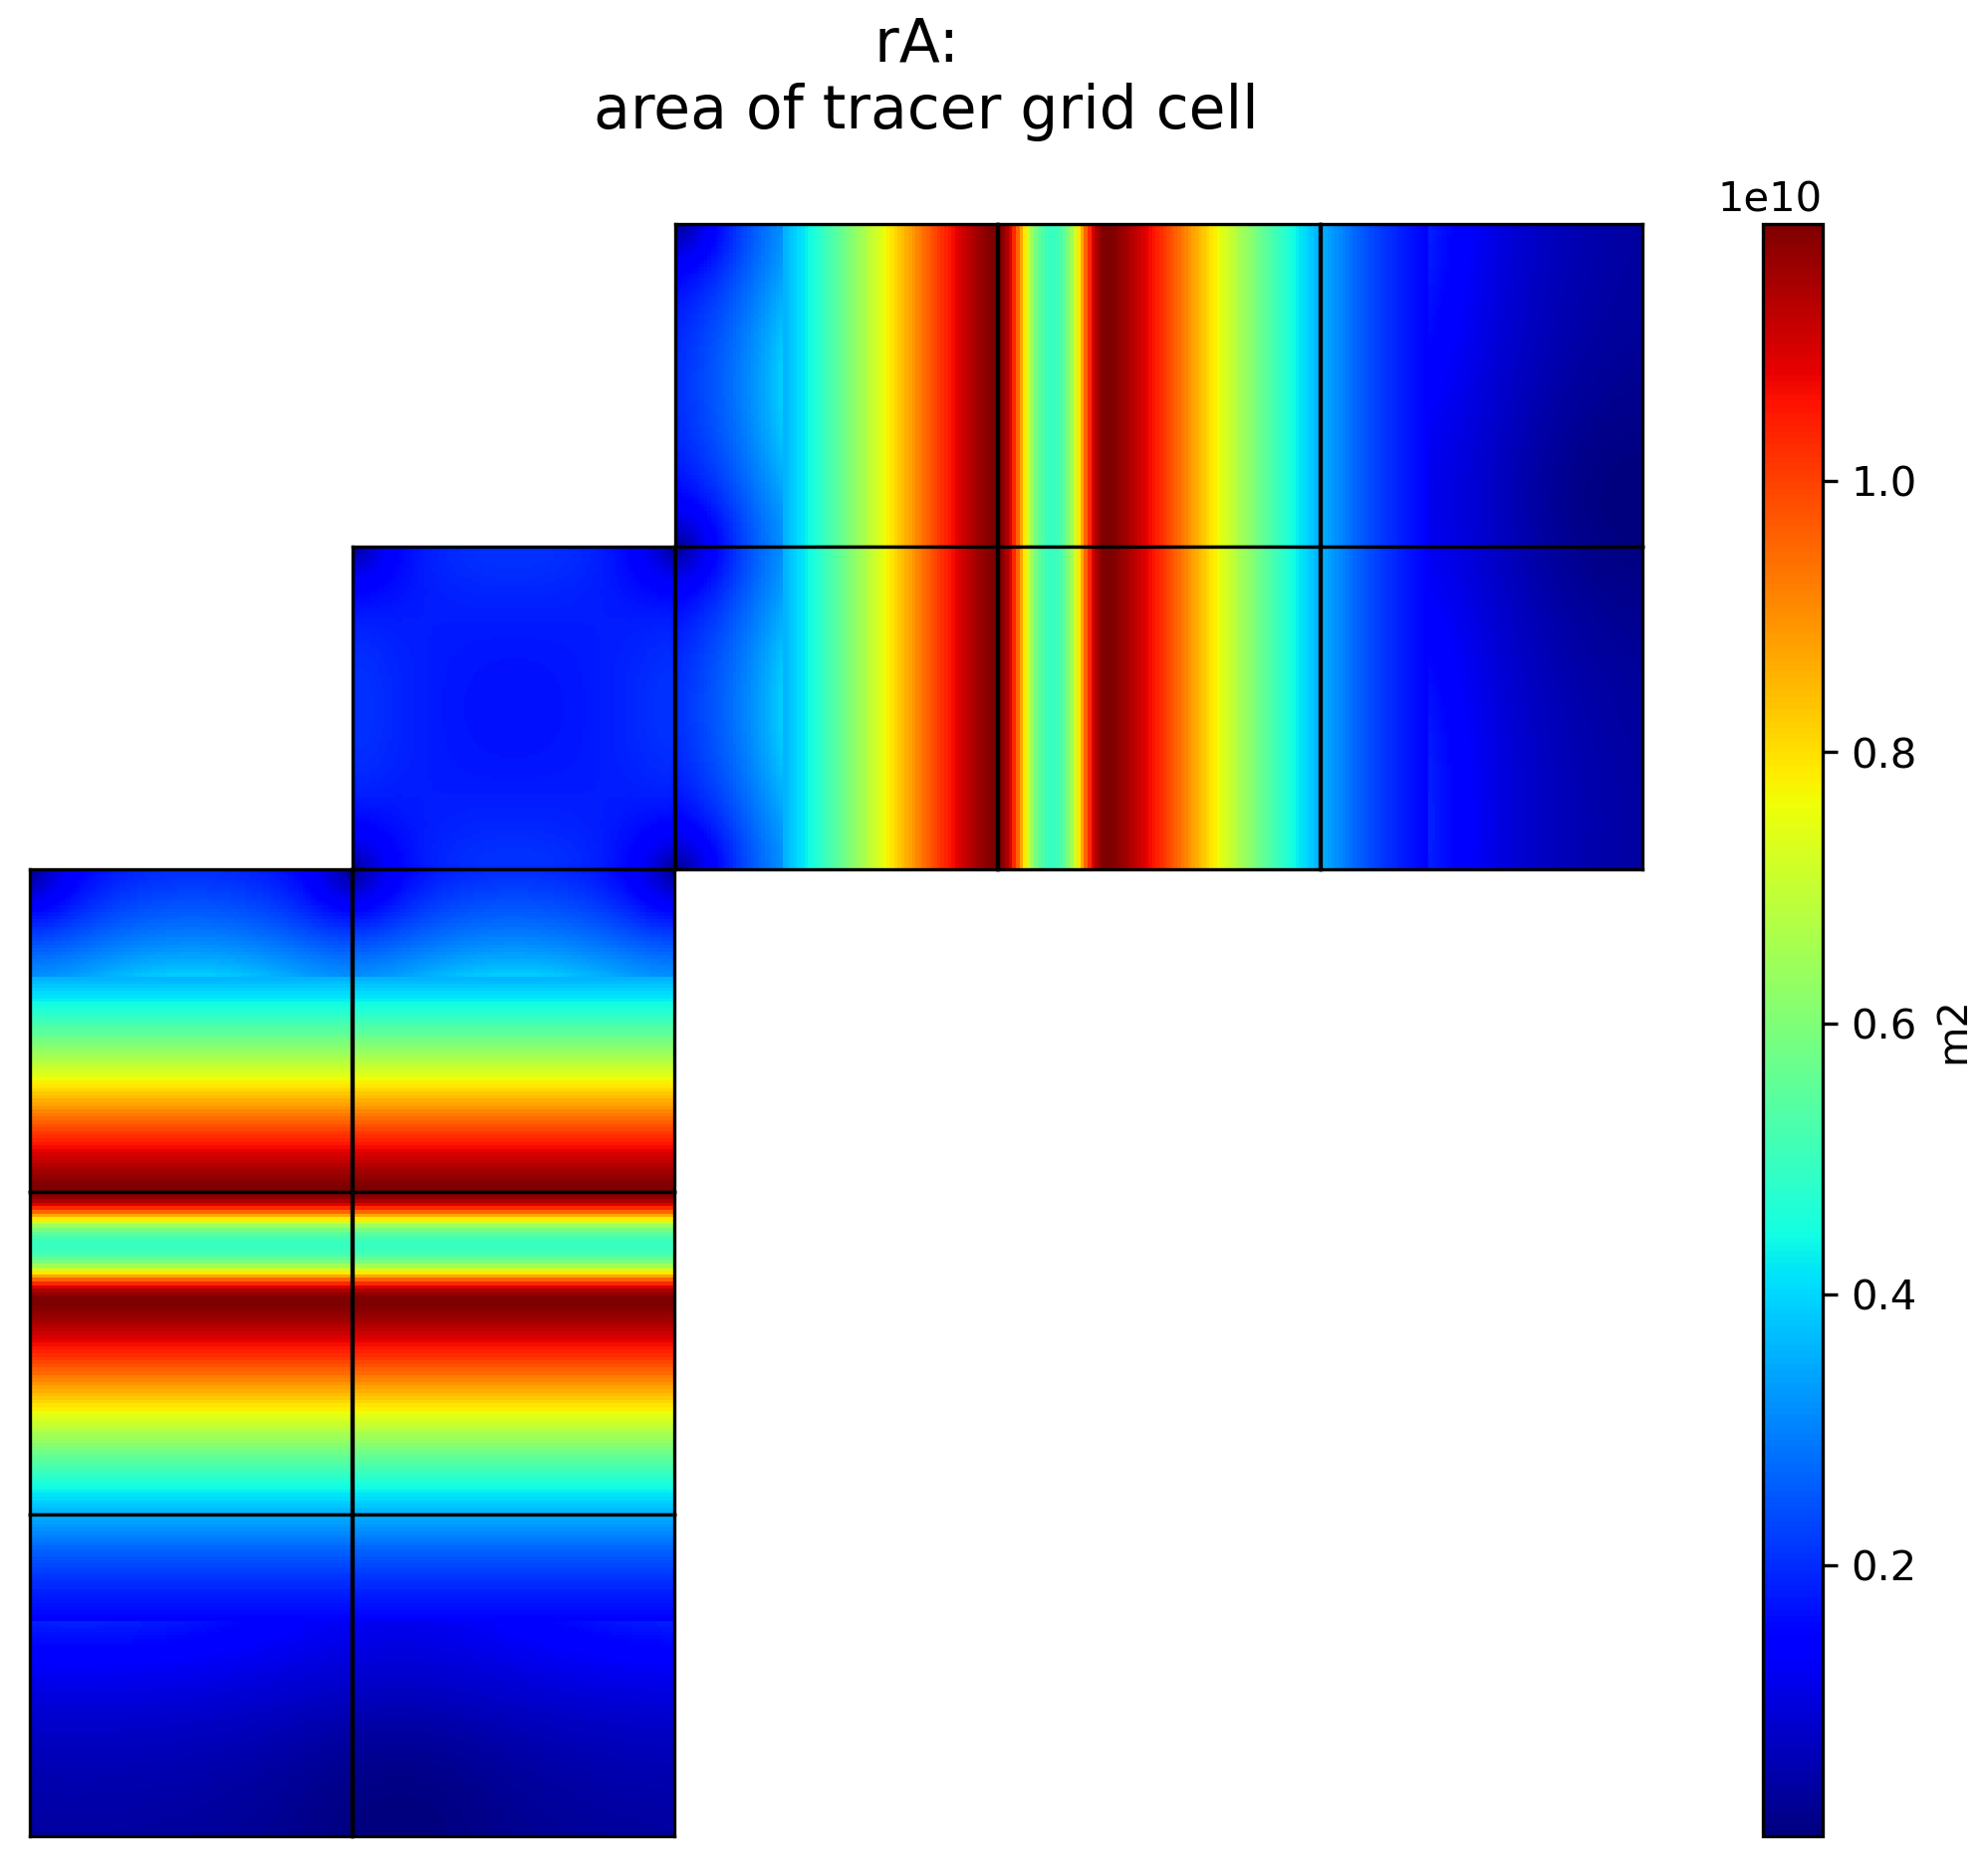
\includegraphics[scale=0.55]{../images/plots/native_plots_coords/Geometry_Parameters_for_the_Lat-Lon-Cap_90_(llc90)_Native_Model_Grid_(Version_4_Release_4)/rA.png}
\caption{Dataset: GRID\_GEOMETRY\_ECCO, Variable: rA}
\label{tab:table-GRID_GEOMETRY_ECCO_rA-Plot}
\end{figure}
\pagebreak
\subsubsection{Native coordinates Variable: dxG}
\begin{longtable}{|m{0.06\textwidth}|m{0.3\textwidth}|m{0.45\textwidth}|m{0.11\textwidth}|}
\caption{Attributes description of the variable 'dxG' from GRID\_GEOMETRY\_ECCO's  dataset.}
\label{tab:table-GRID_GEOMETRY_ECCO_dxG} \\ 
\hline \endhead \hline \endfoot
\rowcolor{lightgray} \textbf{Storage Type} & \textbf{Variable Name} & \textbf{Description} & \textbf{Unit} \\ \hline
float32 & dxG & Distance between 'southwest' and 'southeast' corners of the tracer grid cell & m \\ \hline
\multicolumn{4}{|c|}{\cellcolor{lightgray}{\textbf{Description of the variable in Common Data language (CDL)}}} \\ \hline
\multicolumn{4}{|c|}{\makecell{\parbox{.92\textwidth}{float32 dxG(tile, j\_g, i)\\
\hspace*{0.5cm}dxG: \_FillValue = 9.96921e+36\\
\hspace*{0.5cm}dxG: long\_name = "distance between southwest and southeast corners of the tracer grid cell"\\
\hspace*{0.5cm}dxG: units = m\\
\hspace*{0.5cm}dxG: coordinate = YG XC\\
\hspace*{0.5cm}dxG: coverage\_content\_type = modelResult}}} \\ \hline
\rowcolor{lightgray} \multicolumn{4}{|c|}{\textbf{Comments}} \\ \hline
\multicolumn{4}{|p{1\textwidth}|}{Alternatively, the length of 'south' side of tracer grid cell. note: 'south', 'southwest', and 'southeast' do not correspond to geographic orientation but are used for convenience to describe the computational grid. see mitgcm documentation for details.} \\ \hline
\end{longtable}

\begin{figure}[H]
\centering
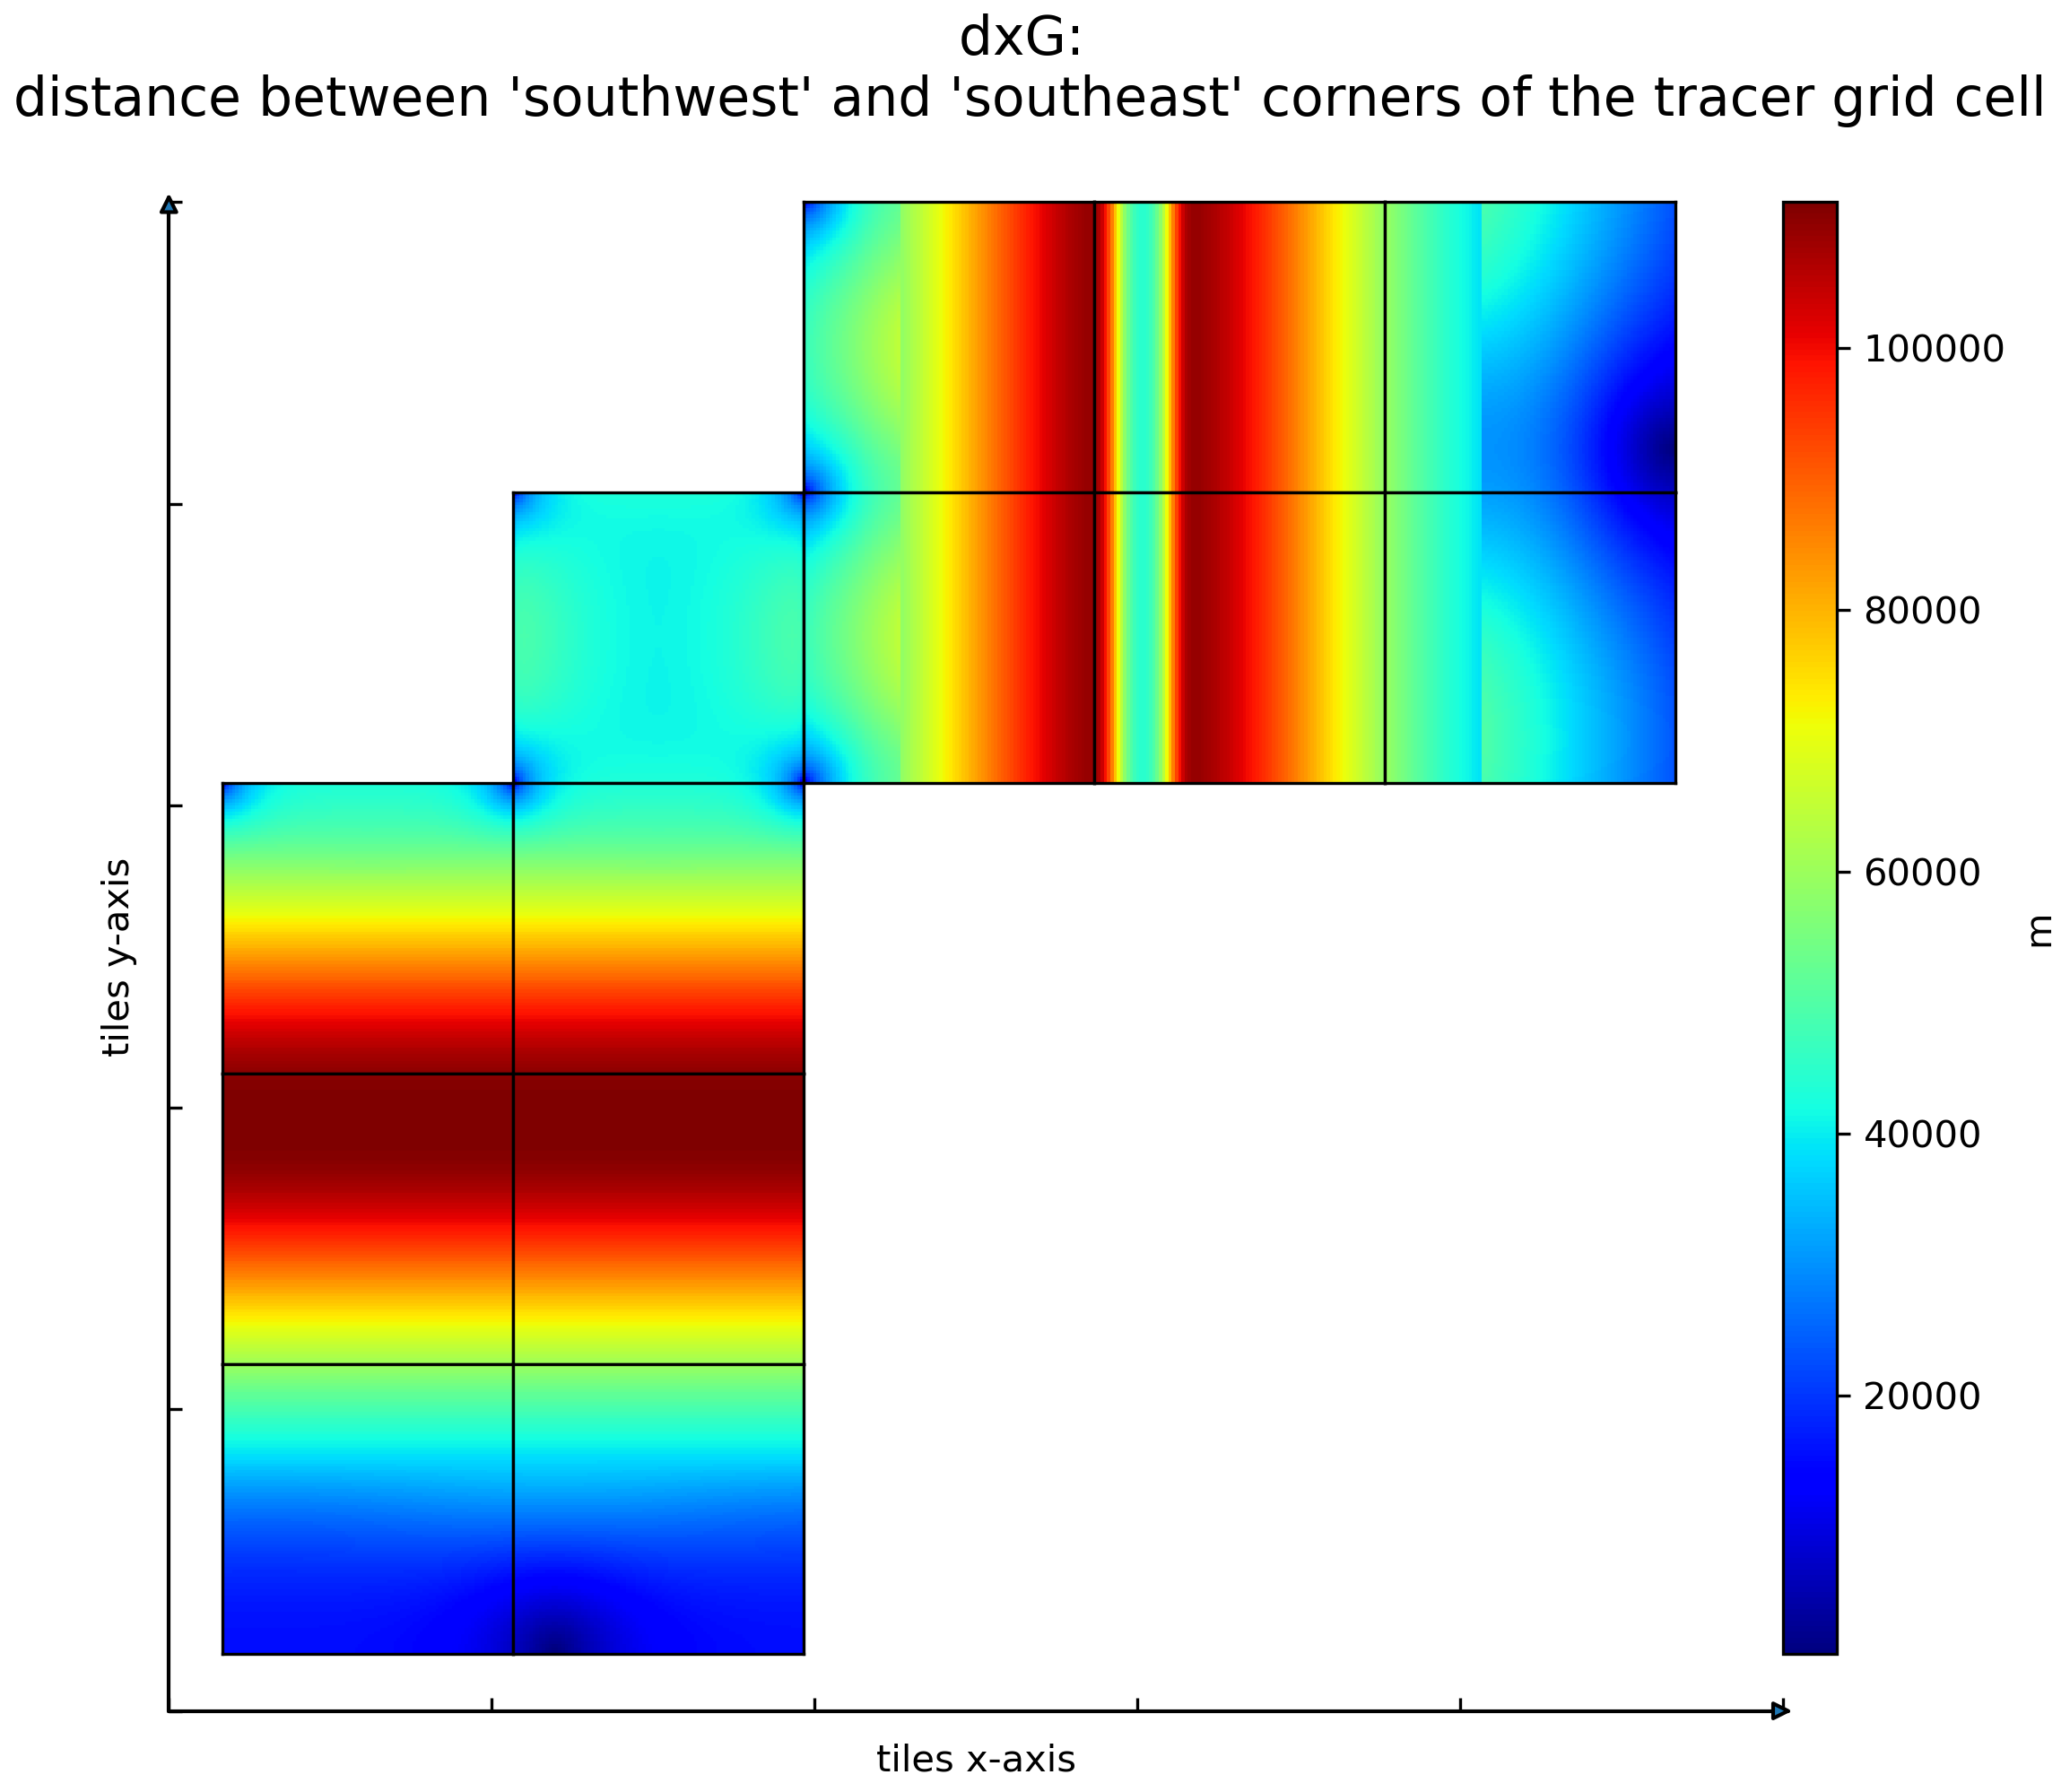
\includegraphics[scale=0.55]{../images/plots/native_plots_coords/Geometry_Parameters_for_the_Lat-Lon-Cap_90_(llc90)_Native_Model_Grid_(Version_4_Release_4)/dxG.png}
\caption{Dataset: GRID\_GEOMETRY\_ECCO, Variable: dxG}
\label{tab:table-GRID_GEOMETRY_ECCO_dxG-Plot}
\end{figure}
\pagebreak
\subsubsection{Native coordinates Variable: dyG}
\begin{longtable}{|m{0.06\textwidth}|m{0.3\textwidth}|m{0.45\textwidth}|m{0.11\textwidth}|}
\caption{Attributes description of the variable 'dyG' from GRID\_GEOMETRY\_ECCO's  dataset.}
\label{tab:table-GRID_GEOMETRY_ECCO_dyG} \\ 
\hline \endhead \hline \endfoot
\rowcolor{lightgray} \textbf{Storage Type} & \textbf{Variable Name} & \textbf{Description} & \textbf{Unit} \\ \hline
float32 & dyG & Distance between 'southwest' and 'northwest' corners of the tracer grid cell & m \\ \hline
\multicolumn{4}{|c|}{\cellcolor{lightgray}{\textbf{Description of the variable in Common Data language (CDL)}}} \\ \hline
\multicolumn{4}{|c|}{\makecell{\parbox{.92\textwidth}{float32 dyG(tile, j, i\_g)\\
\hspace*{0.5cm}dyG: \_FillValue = 9.96921e+36\\
\hspace*{0.5cm}dyG: long\_name = "distance between southwest and northwest corners of the tracer grid cell"\\
\hspace*{0.5cm}dyG: units = m\\
\hspace*{0.5cm}dyG: coordinate = YC XG\\
\hspace*{0.5cm}dyG: coverage\_content\_type = modelResult}}} \\ \hline
\rowcolor{lightgray} \multicolumn{4}{|c|}{\textbf{Comments}} \\ \hline
\multicolumn{4}{|p{1\textwidth}|}{Alternatively, the length of 'west' side of tracer grid cell. note: 'west, 'southwest', and 'northwest' do not correspond to geographic orientation but are used for convenience to describe the computational grid. see mitgcm documentation for details.} \\ \hline
\end{longtable}

\begin{figure}[H]
\centering
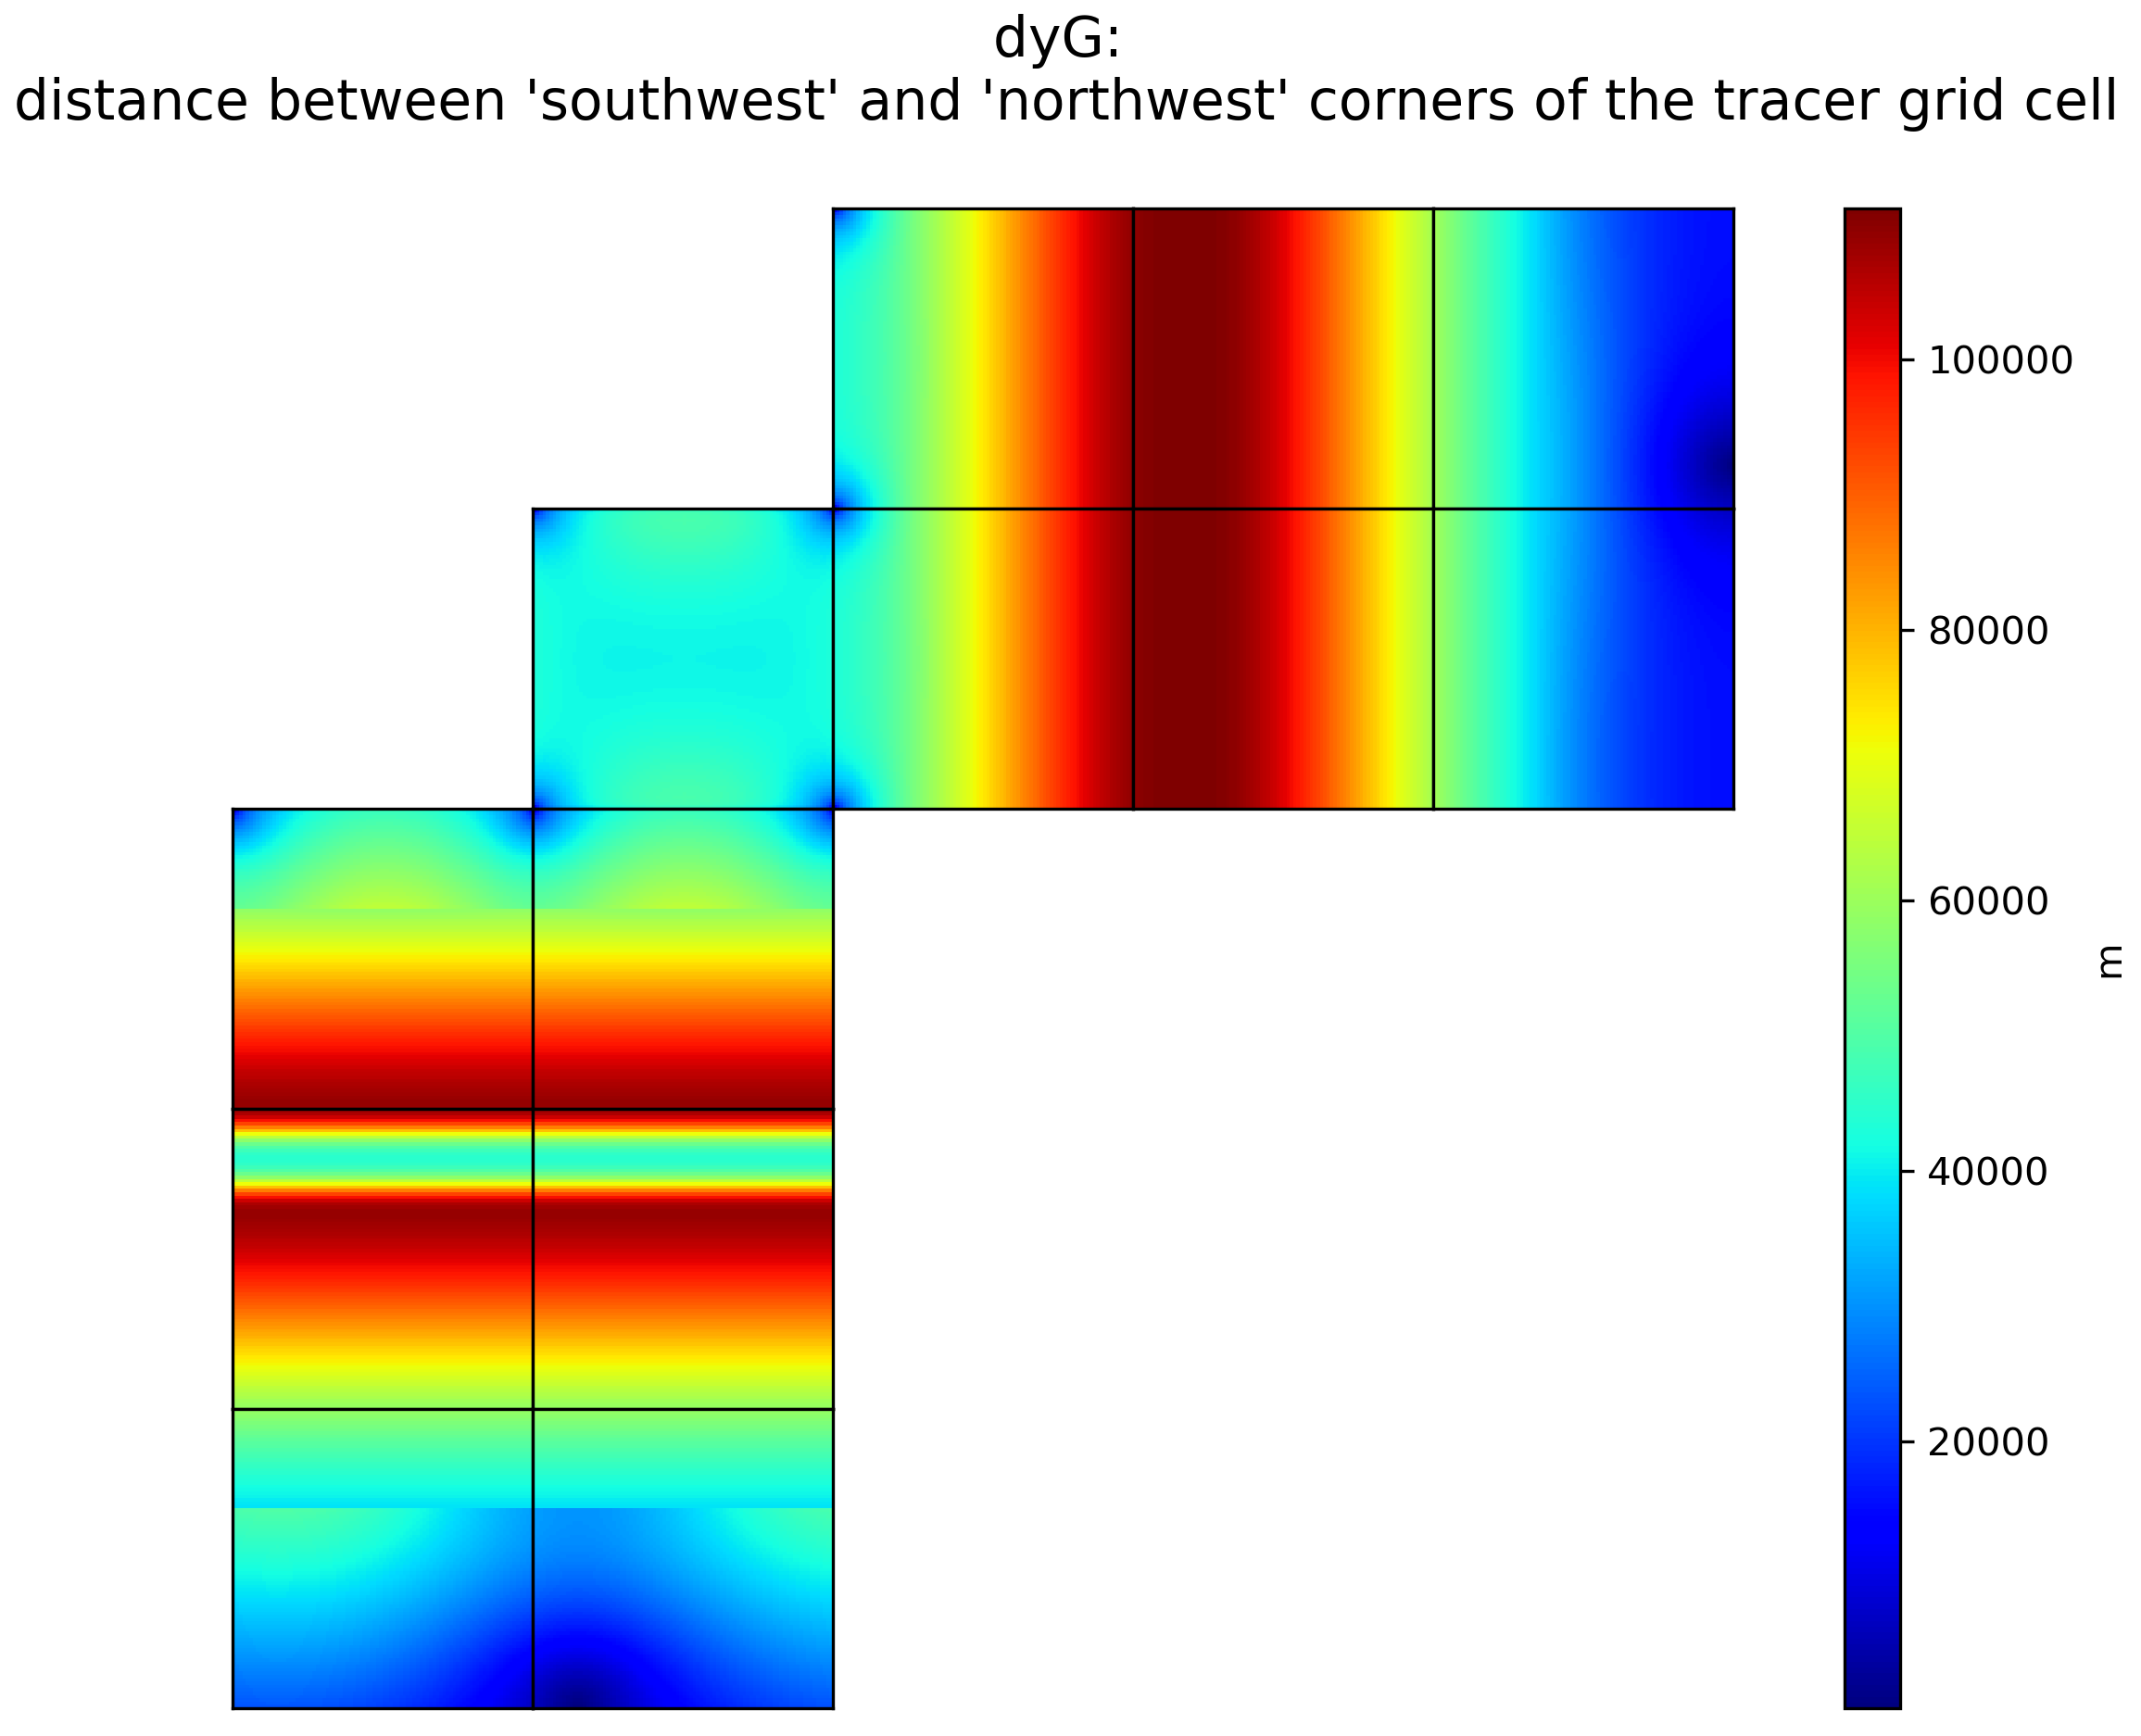
\includegraphics[scale=0.55]{../images/plots/native_plots_coords/Geometry_Parameters_for_the_Lat-Lon-Cap_90_(llc90)_Native_Model_Grid_(Version_4_Release_4)/dyG.png}
\caption{Dataset: GRID\_GEOMETRY\_ECCO, Variable: dyG}
\label{tab:table-GRID_GEOMETRY_ECCO_dyG-Plot}
\end{figure}
\pagebreak
\subsubsection{Native coordinates Variable: Depth}
\begin{longtable}{|m{0.06\textwidth}|m{0.3\textwidth}|m{0.45\textwidth}|m{0.11\textwidth}|}
\caption{Attributes description of the variable 'Depth' from GRID\_GEOMETRY\_ECCO's  dataset.}
\label{tab:table-GRID_GEOMETRY_ECCO_Depth} \\ 
\hline \endhead \hline \endfoot
\rowcolor{lightgray} \textbf{Storage Type} & \textbf{Variable Name} & \textbf{Description} & \textbf{Unit} \\ \hline
float32 & Depth & Model seafloor depth below ocean surface at rest & m \\ \hline
\multicolumn{4}{|c|}{\cellcolor{lightgray}{\textbf{Description of the variable in Common Data language (CDL)}}} \\ \hline
\multicolumn{4}{|c|}{\makecell{\parbox{.92\textwidth}{float32 Depth(tile, j, i)\\
\hspace*{0.5cm}Depth: \_FillValue = 9.96921e+36\\
\hspace*{0.5cm}Depth: long\_name = model seafloor depth below ocean surface at rest\\
\hspace*{0.5cm}Depth: units = m\\
\hspace*{0.5cm}Depth: coordinate = XC YC\\
\hspace*{0.5cm}Depth: coverage\_content\_type = modelResult\\
\hspace*{0.5cm}Depth: standard\_name = sea\_floor\_depth\_below\_geoid\\
\hspace*{0.5cm}Depth: coordinates = YC XC}}} \\ \hline
\rowcolor{lightgray} \multicolumn{4}{|c|}{\textbf{Comments}} \\ \hline
\multicolumn{4}{|p{1\textwidth}|}{Model sea surface height (ssh) of 0m corresponds to an ocean surface at rest relative to the geoid. depth corresponds to seafloor depth below geoid. note: the mitgcm used by ecco v4r4 implements 'partial cells' so the actual model seafloor depth may differ from the seafloor depth provided by the input bathymetry file.} \\ \hline
\end{longtable}

\begin{figure}[H]
\centering
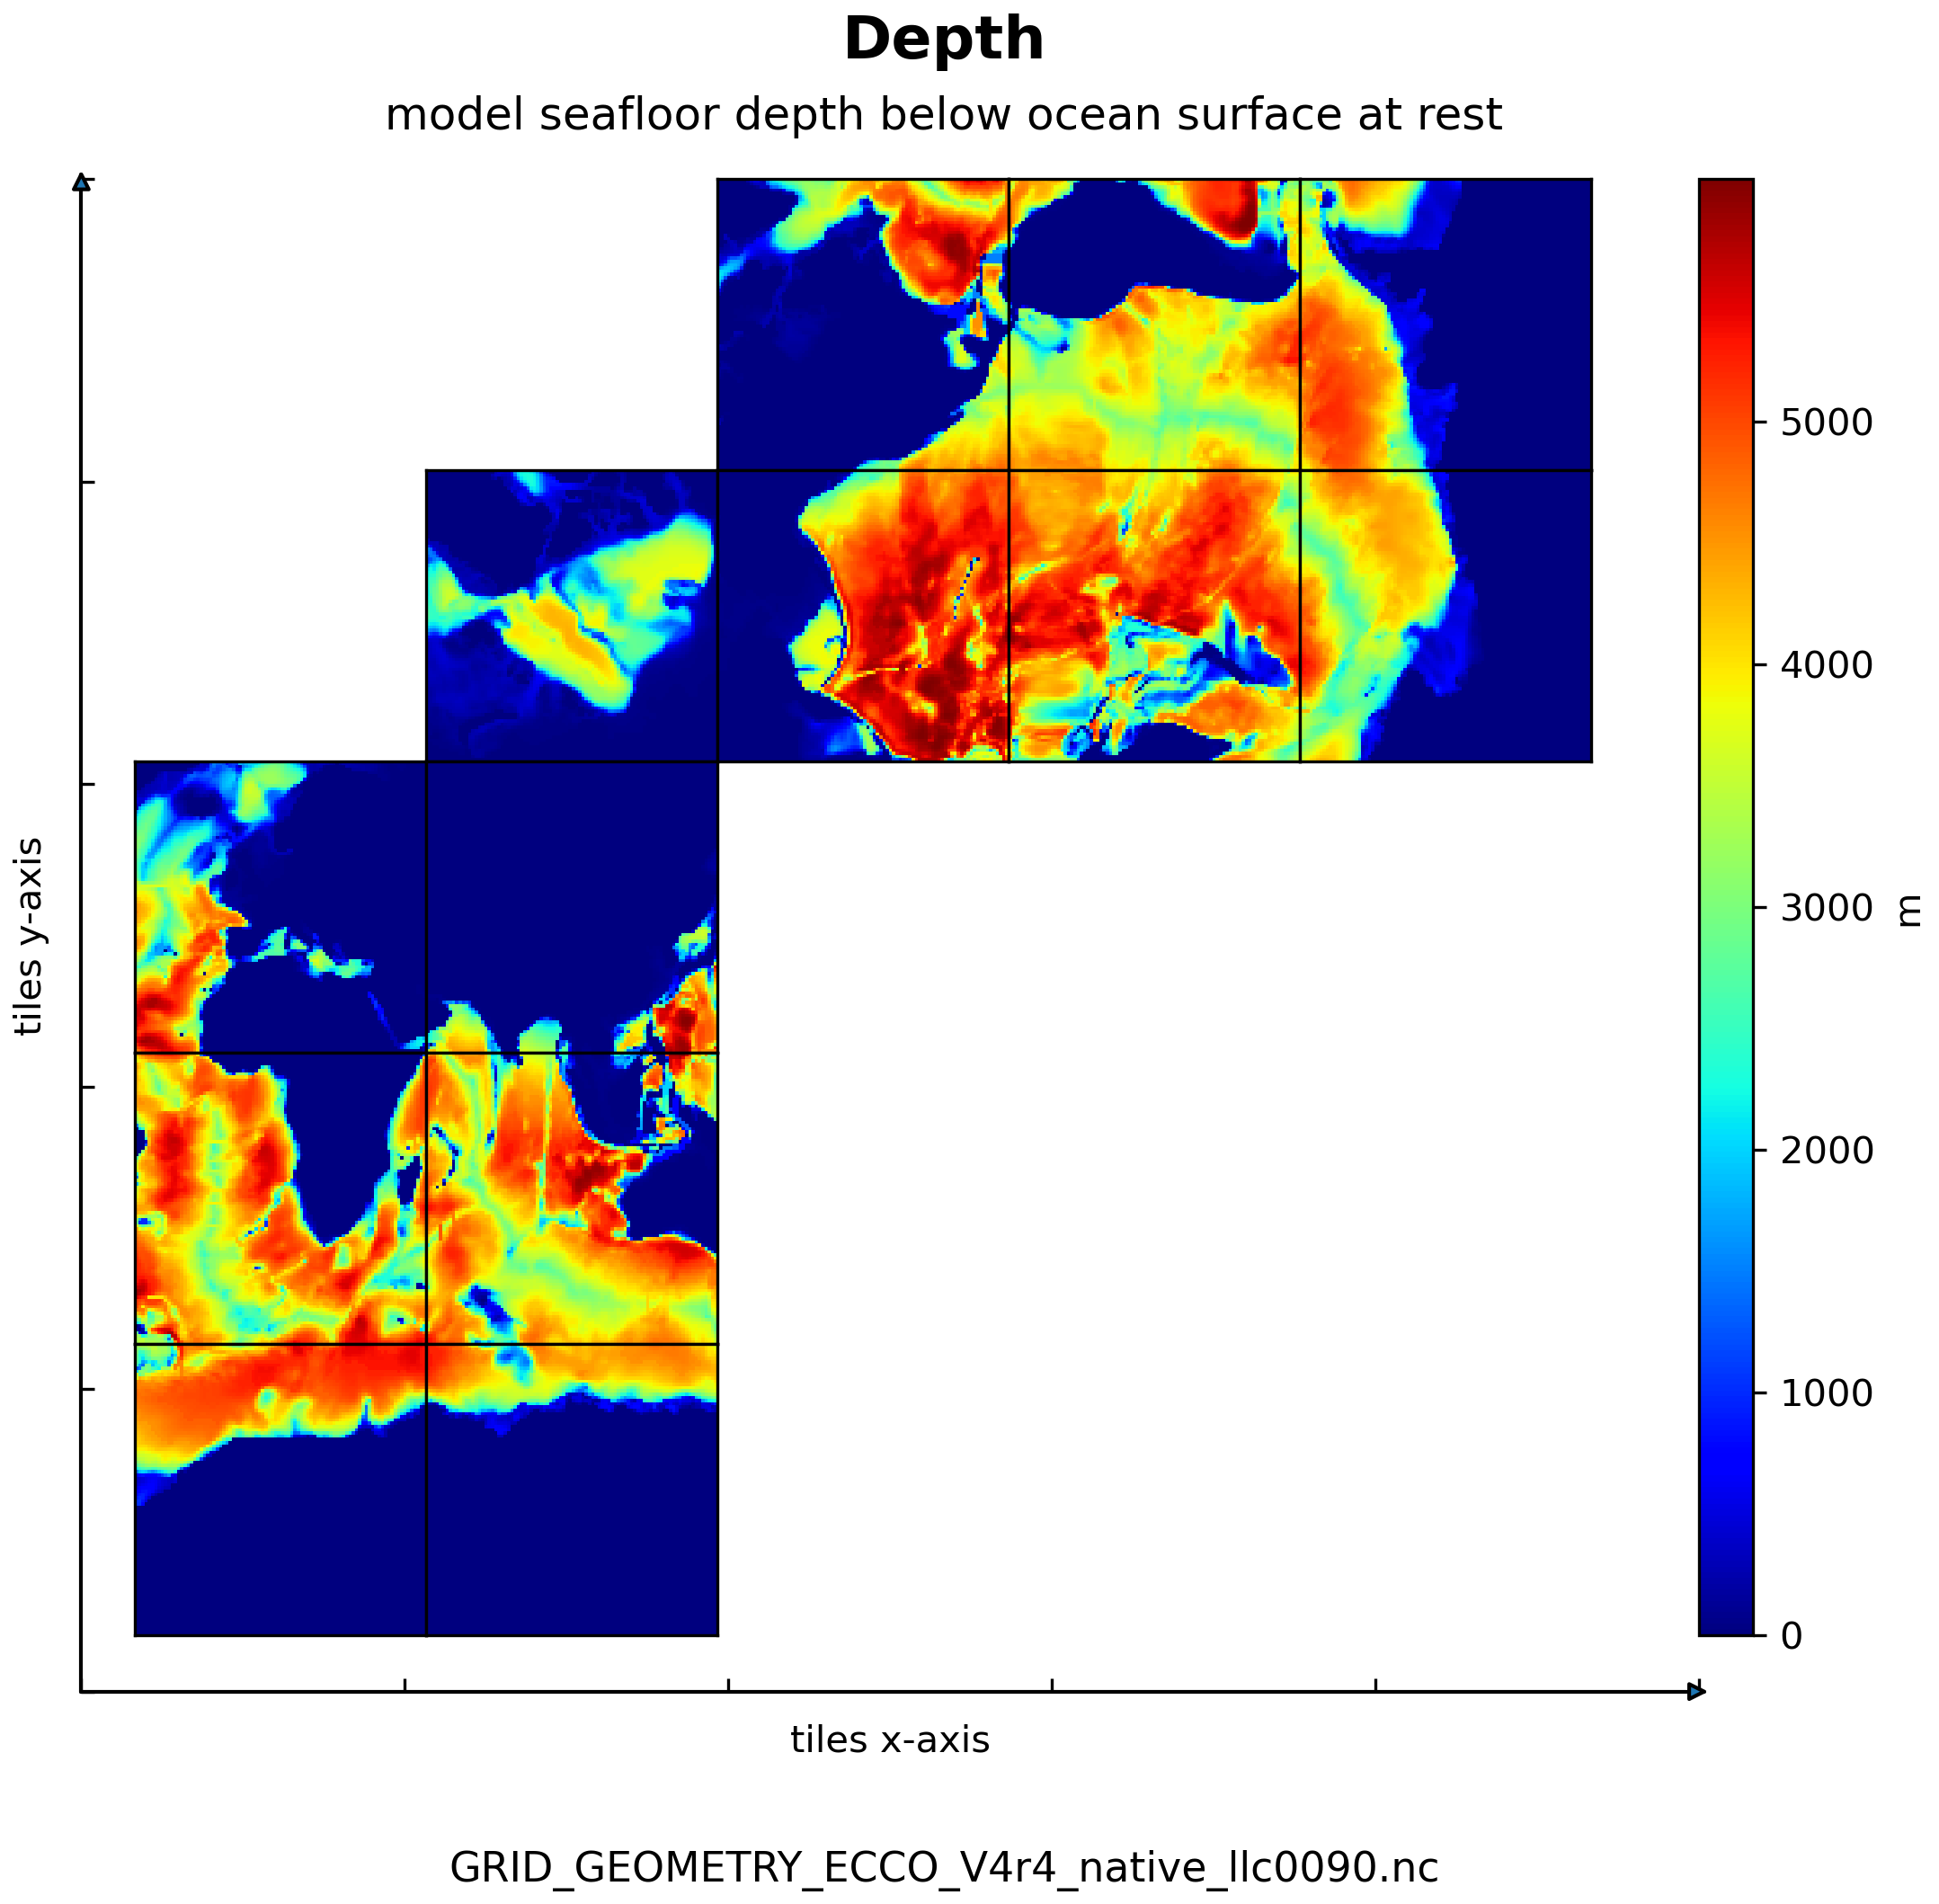
\includegraphics[scale=0.55]{../images/plots/native_plots_coords/Geometry_Parameters_for_the_Lat-Lon-Cap_90_(llc90)_Native_Model_Grid_(Version_4_Release_4)/Depth.png}
\caption{Dataset: GRID\_GEOMETRY\_ECCO, Variable: Depth}
\label{tab:table-GRID_GEOMETRY_ECCO_Depth-Plot}
\end{figure}
\pagebreak
\subsubsection{Native coordinates Variable: rAz}
\begin{longtable}{|m{0.06\textwidth}|m{0.3\textwidth}|m{0.45\textwidth}|m{0.11\textwidth}|}
\caption{Attributes description of the variable 'rAz' from GRID\_GEOMETRY\_ECCO's  dataset.}
\label{tab:table-GRID_GEOMETRY_ECCO_rAz} \\ 
\hline \endhead \hline \endfoot
\rowcolor{lightgray} \textbf{Storage Type} & \textbf{Variable Name} & \textbf{Description} & \textbf{Unit} \\ \hline
float32 & rAz & Area of vorticity 'g' grid cell & m2 \\ \hline
\multicolumn{4}{|c|}{\cellcolor{lightgray}{\textbf{Description of the variable in Common Data language (CDL)}}} \\ \hline
\multicolumn{4}{|c|}{\makecell{\parbox{.92\textwidth}{float32 rAz(tile, j\_g, i\_g)\\
\hspace*{0.5cm}rAz: \_FillValue = 9.96921e+36\\
\hspace*{0.5cm}rAz: long\_name = "area of vorticity g grid cell"\\
\hspace*{0.5cm}rAz: units = m2\\
\hspace*{0.5cm}rAz: coordinate = YG XG\\
\hspace*{0.5cm}rAz: coverage\_content\_type = modelResult\\
\hspace*{0.5cm}rAz: standard\_name = cell\_area\\
\hspace*{0.5cm}rAz: coordinates = YG XG}}} \\ \hline
\rowcolor{lightgray} \multicolumn{4}{|c|}{\textbf{Comments}} \\ \hline
\multicolumn{4}{|p{1\textwidth}|}{Vorticity cells are staggered in space relative to tracer cells, nominally situated on tracer cell corners. vorticity cell (i,j) is located at the 'southwest' corner of tracer grid cell (i, j). note: 'southwest' does not correspond to geographic orientation but is used for convenience to describe the computational grid. see mitgcm documentation for details.} \\ \hline
\end{longtable}

\begin{figure}[H]
\centering
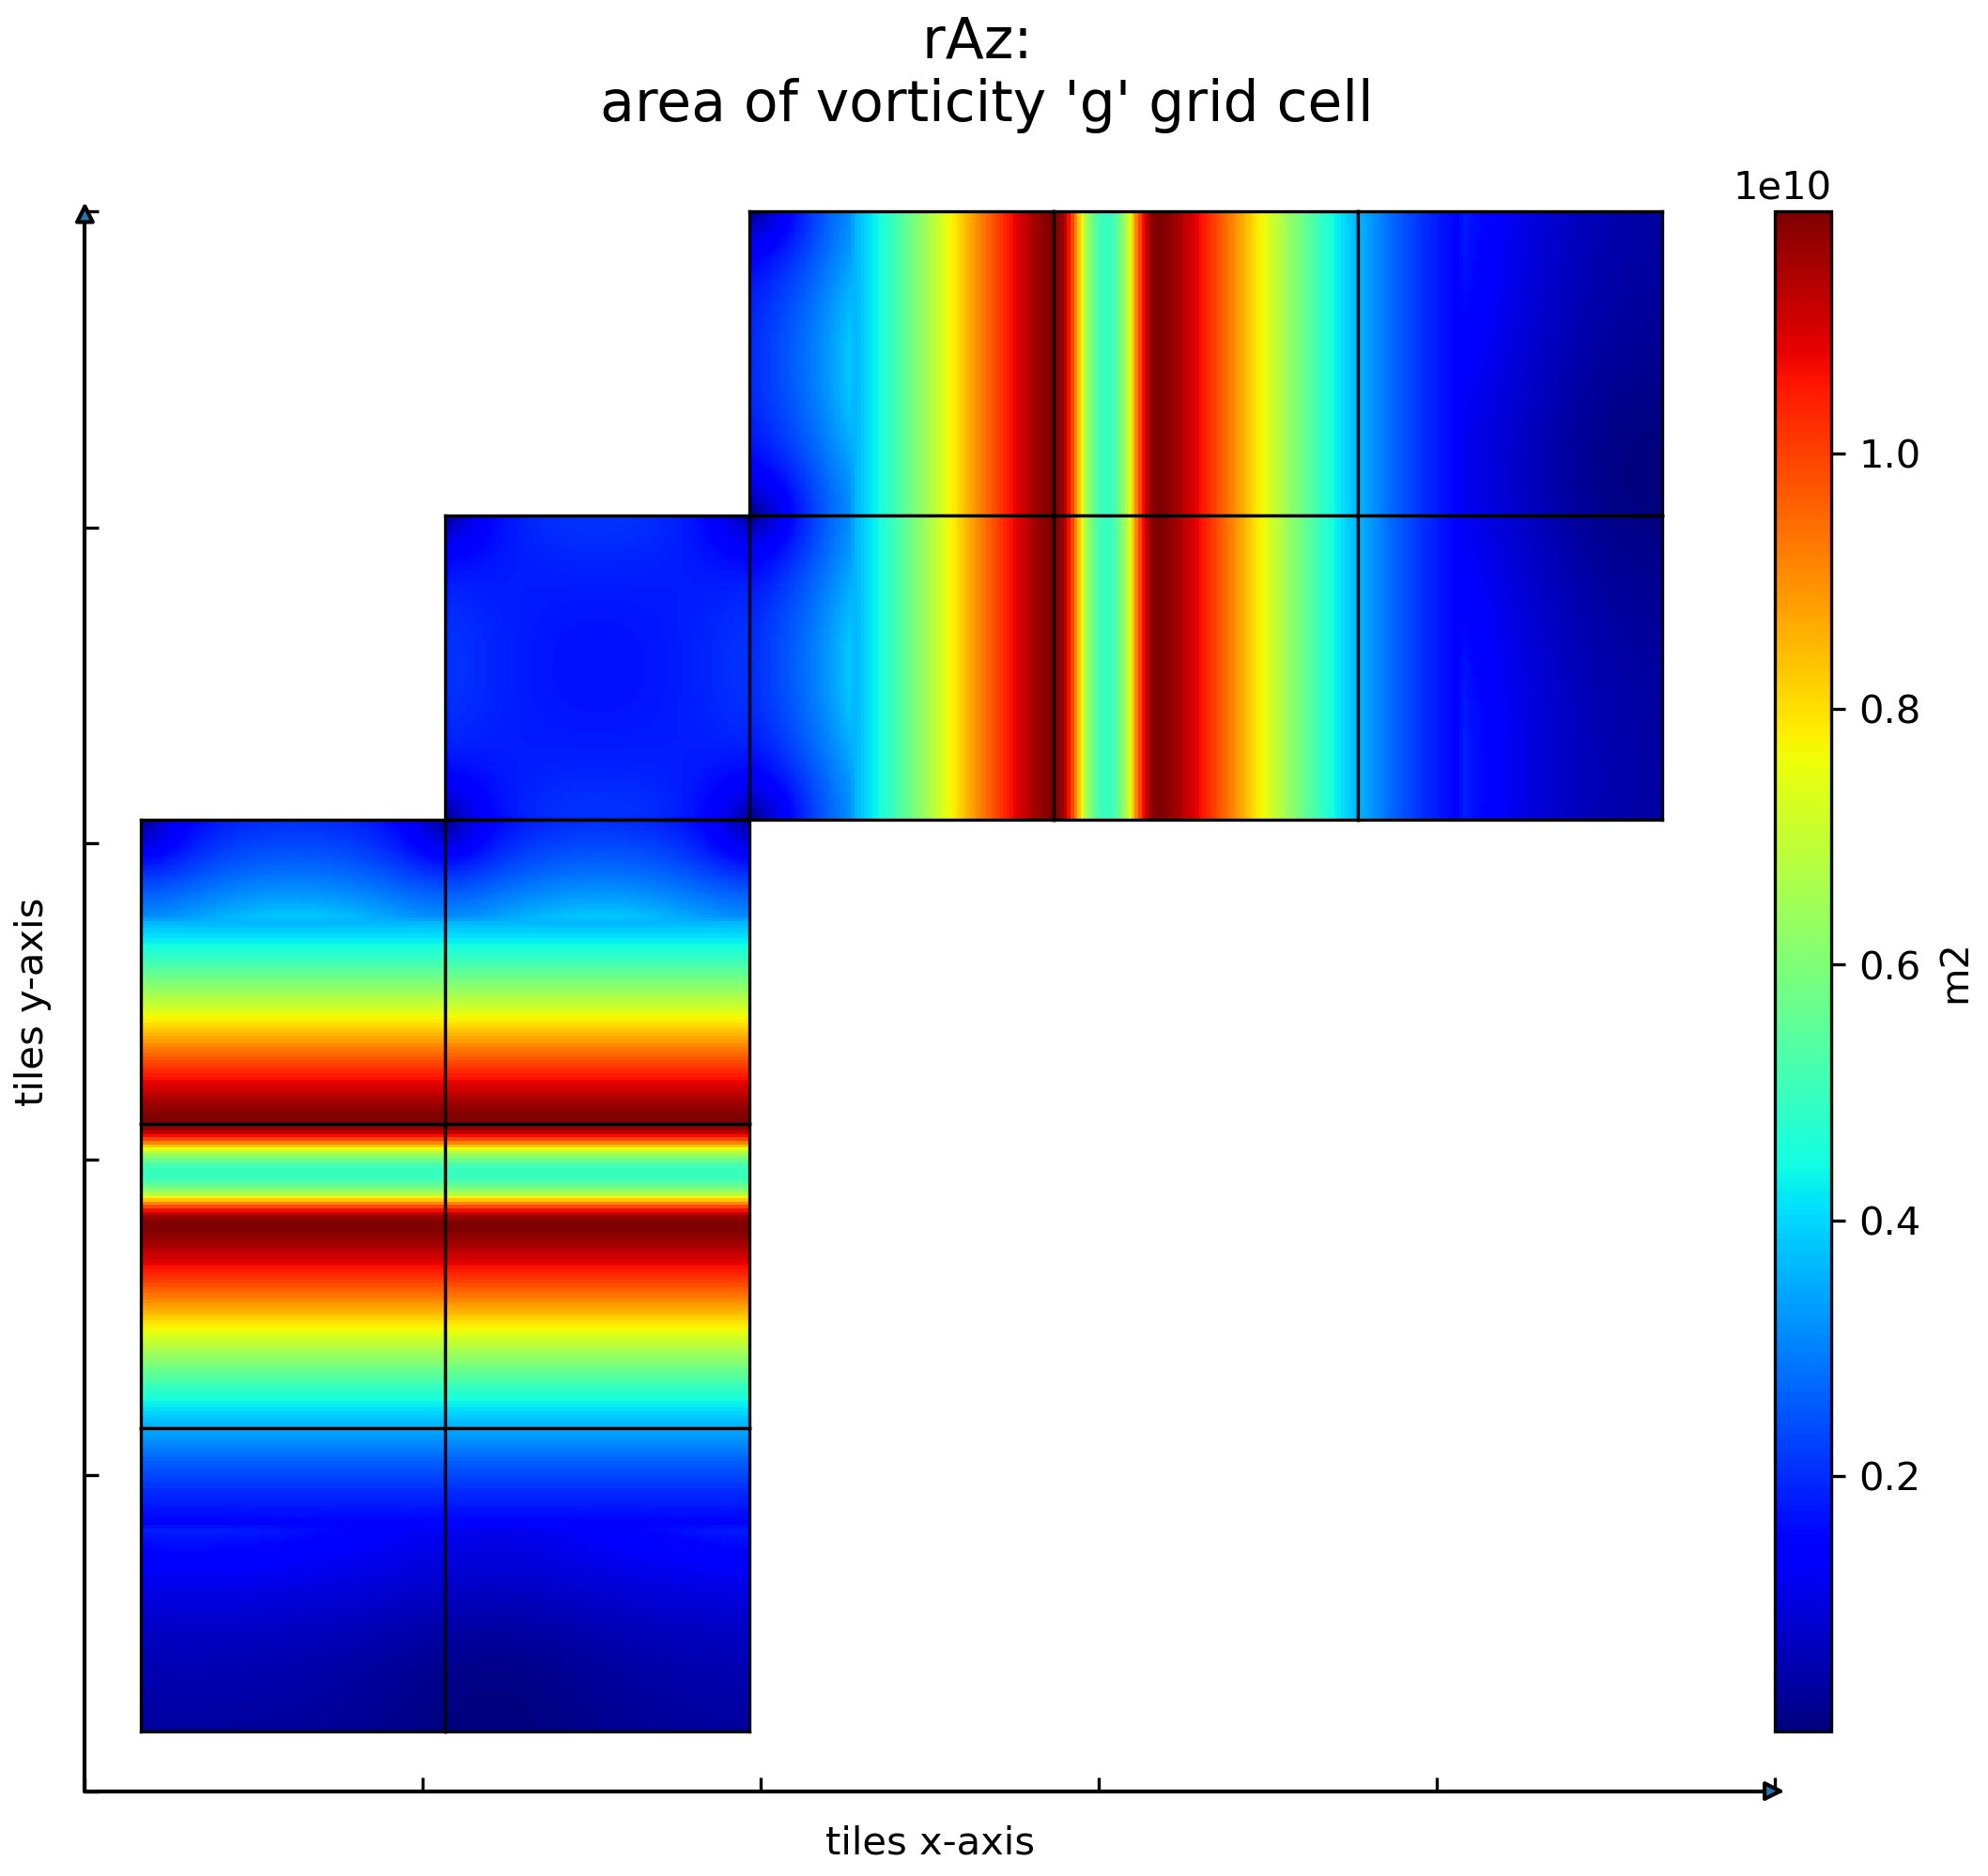
\includegraphics[scale=0.55]{../images/plots/native_plots_coords/Geometry_Parameters_for_the_Lat-Lon-Cap_90_(llc90)_Native_Model_Grid_(Version_4_Release_4)/rAz.png}
\caption{Dataset: GRID\_GEOMETRY\_ECCO, Variable: rAz}
\label{tab:table-GRID_GEOMETRY_ECCO_rAz-Plot}
\end{figure}
\pagebreak
\subsubsection{Native coordinates Variable: dxC}
\begin{longtable}{|m{0.06\textwidth}|m{0.3\textwidth}|m{0.45\textwidth}|m{0.11\textwidth}|}
\caption{Attributes description of the variable 'dxC' from GRID\_GEOMETRY\_ECCO's  dataset.}
\label{tab:table-GRID_GEOMETRY_ECCO_dxC} \\ 
\hline \endhead \hline \endfoot
\rowcolor{lightgray} \textbf{Storage Type} & \textbf{Variable Name} & \textbf{Description} & \textbf{Unit} \\ \hline
float32 & dxC & Distance between centers of adjacent tracer grid cells in the 'x' direction & m \\ \hline
\multicolumn{4}{|c|}{\cellcolor{lightgray}{\textbf{Description of the variable in Common Data language (CDL)}}} \\ \hline
\multicolumn{4}{|c|}{\makecell{\parbox{.92\textwidth}{float32 dxC(tile, j, i\_g)\\
\hspace*{0.5cm}dxC: \_FillValue = 9.96921e+36\\
\hspace*{0.5cm}dxC: long\_name = "distance between centers of adjacent tracer grid cells in the x direction"\\
\hspace*{0.5cm}dxC: units = m\\
\hspace*{0.5cm}dxC: coordinate = YC XG\\
\hspace*{0.5cm}dxC: coverage\_content\_type = modelResult}}} \\ \hline
\rowcolor{lightgray} \multicolumn{4}{|c|}{\textbf{Comments}} \\ \hline
\multicolumn{4}{|p{1\textwidth}|}{Alternatively, the length of 'north' side of vorticity grid cells. note: 'north' does not correspond to geographic orientation but is used for convenience to describe the computational grid. see mitgcm documentation for details.} \\ \hline
\end{longtable}

\begin{figure}[H]
\centering
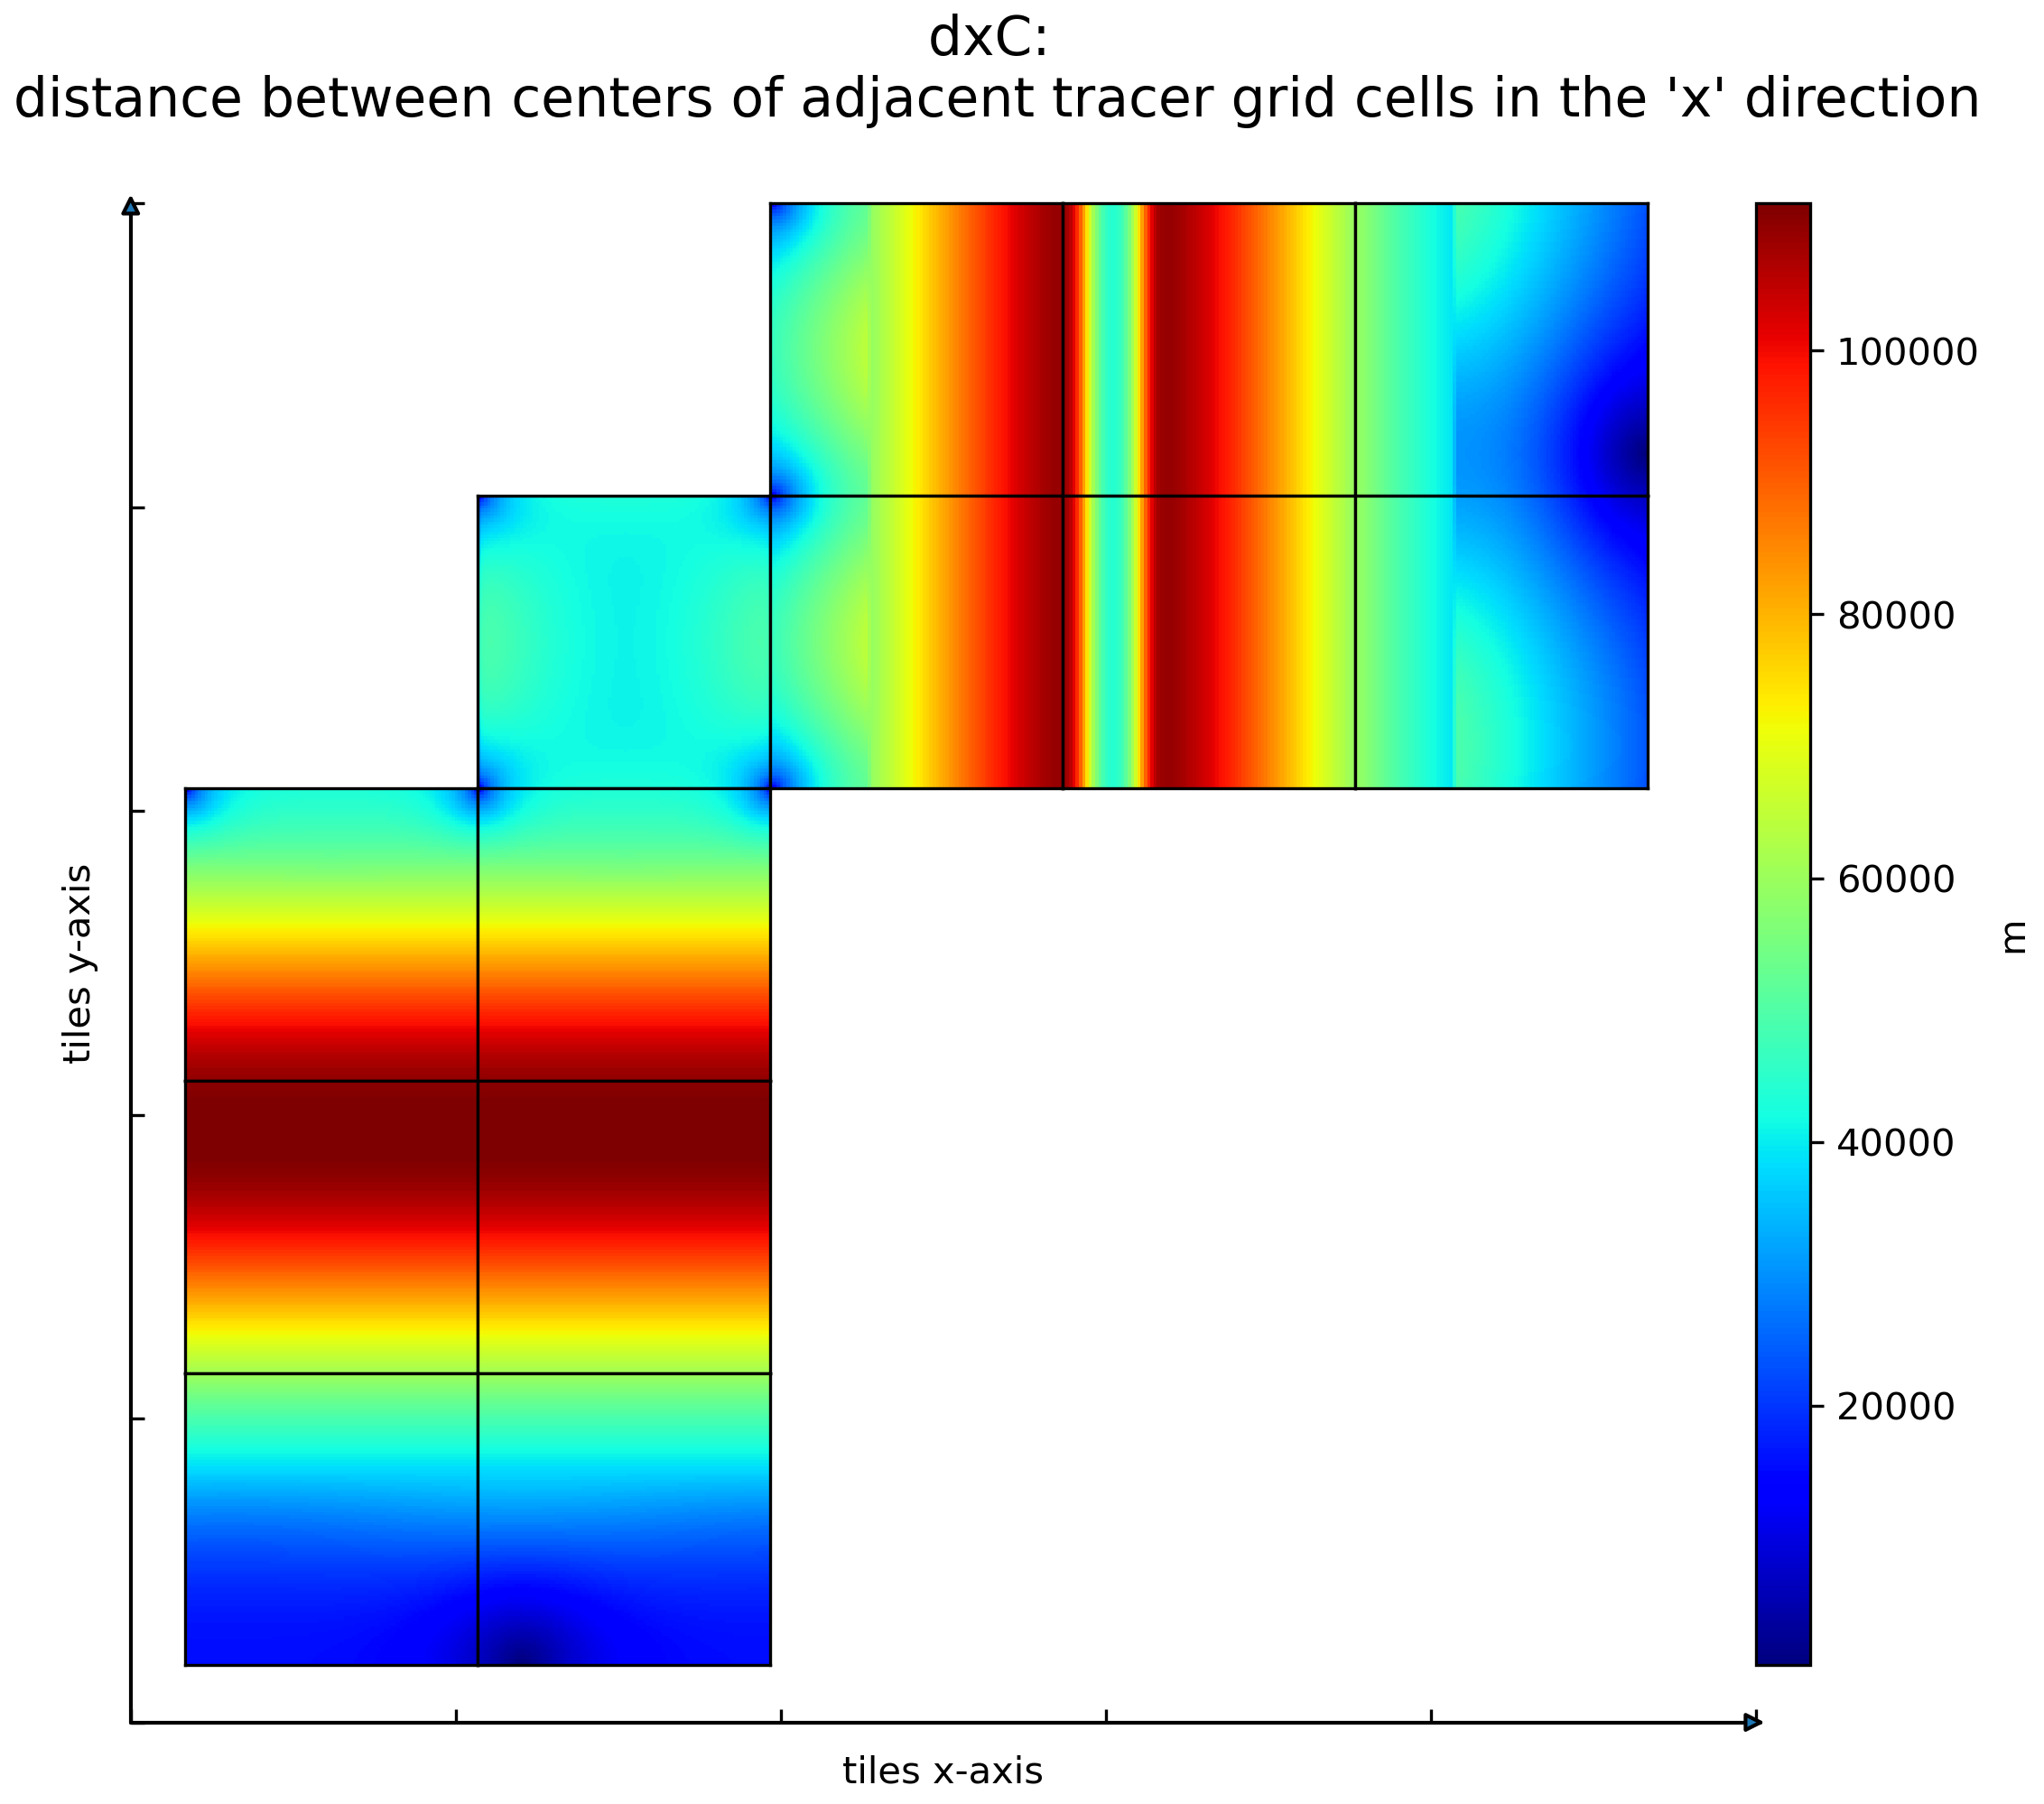
\includegraphics[scale=0.55]{../images/plots/native_plots_coords/Geometry_Parameters_for_the_Lat-Lon-Cap_90_(llc90)_Native_Model_Grid_(Version_4_Release_4)/dxC.png}
\caption{Dataset: GRID\_GEOMETRY\_ECCO, Variable: dxC}
\label{tab:table-GRID_GEOMETRY_ECCO_dxC-Plot}
\end{figure}
\pagebreak
\subsubsection{Native coordinates Variable: dyC}
\begin{longtable}{|m{0.06\textwidth}|m{0.3\textwidth}|m{0.45\textwidth}|m{0.11\textwidth}|}
\caption{Attributes description of the variable 'dyC' from GRID\_GEOMETRY\_ECCO's  dataset.}
\label{tab:table-GRID_GEOMETRY_ECCO_dyC} \\ 
\hline \endhead \hline \endfoot
\rowcolor{lightgray} \textbf{Storage Type} & \textbf{Variable Name} & \textbf{Description} & \textbf{Unit} \\ \hline
float32 & dyC & Distance between centers of adjacent tracer grid cells in the 'y' direction & m \\ \hline
\multicolumn{4}{|c|}{\cellcolor{lightgray}{\textbf{Description of the variable in Common Data language (CDL)}}} \\ \hline
\multicolumn{4}{|c|}{\makecell{\parbox{.92\textwidth}{float32 dyC(tile, j\_g, i)\\
\hspace*{0.5cm}dyC: \_FillValue = 9.96921e+36\\
\hspace*{0.5cm}dyC: long\_name = "distance between centers of adjacent tracer grid cells in the y direction"\\
\hspace*{0.5cm}dyC: units = m\\
\hspace*{0.5cm}dyC: coordinate = YG XC\\
\hspace*{0.5cm}dyC: coverage\_content\_type = modelResult}}} \\ \hline
\rowcolor{lightgray} \multicolumn{4}{|c|}{\textbf{Comments}} \\ \hline
\multicolumn{4}{|p{1\textwidth}|}{Alternatively, the length of 'east' side of vorticity grid cells. note: 'east' does not correspond to geographic orientation but is used for convenience to describe the computational grid. see mitgcm documentation for details.} \\ \hline
\end{longtable}

\begin{figure}[H]
\centering
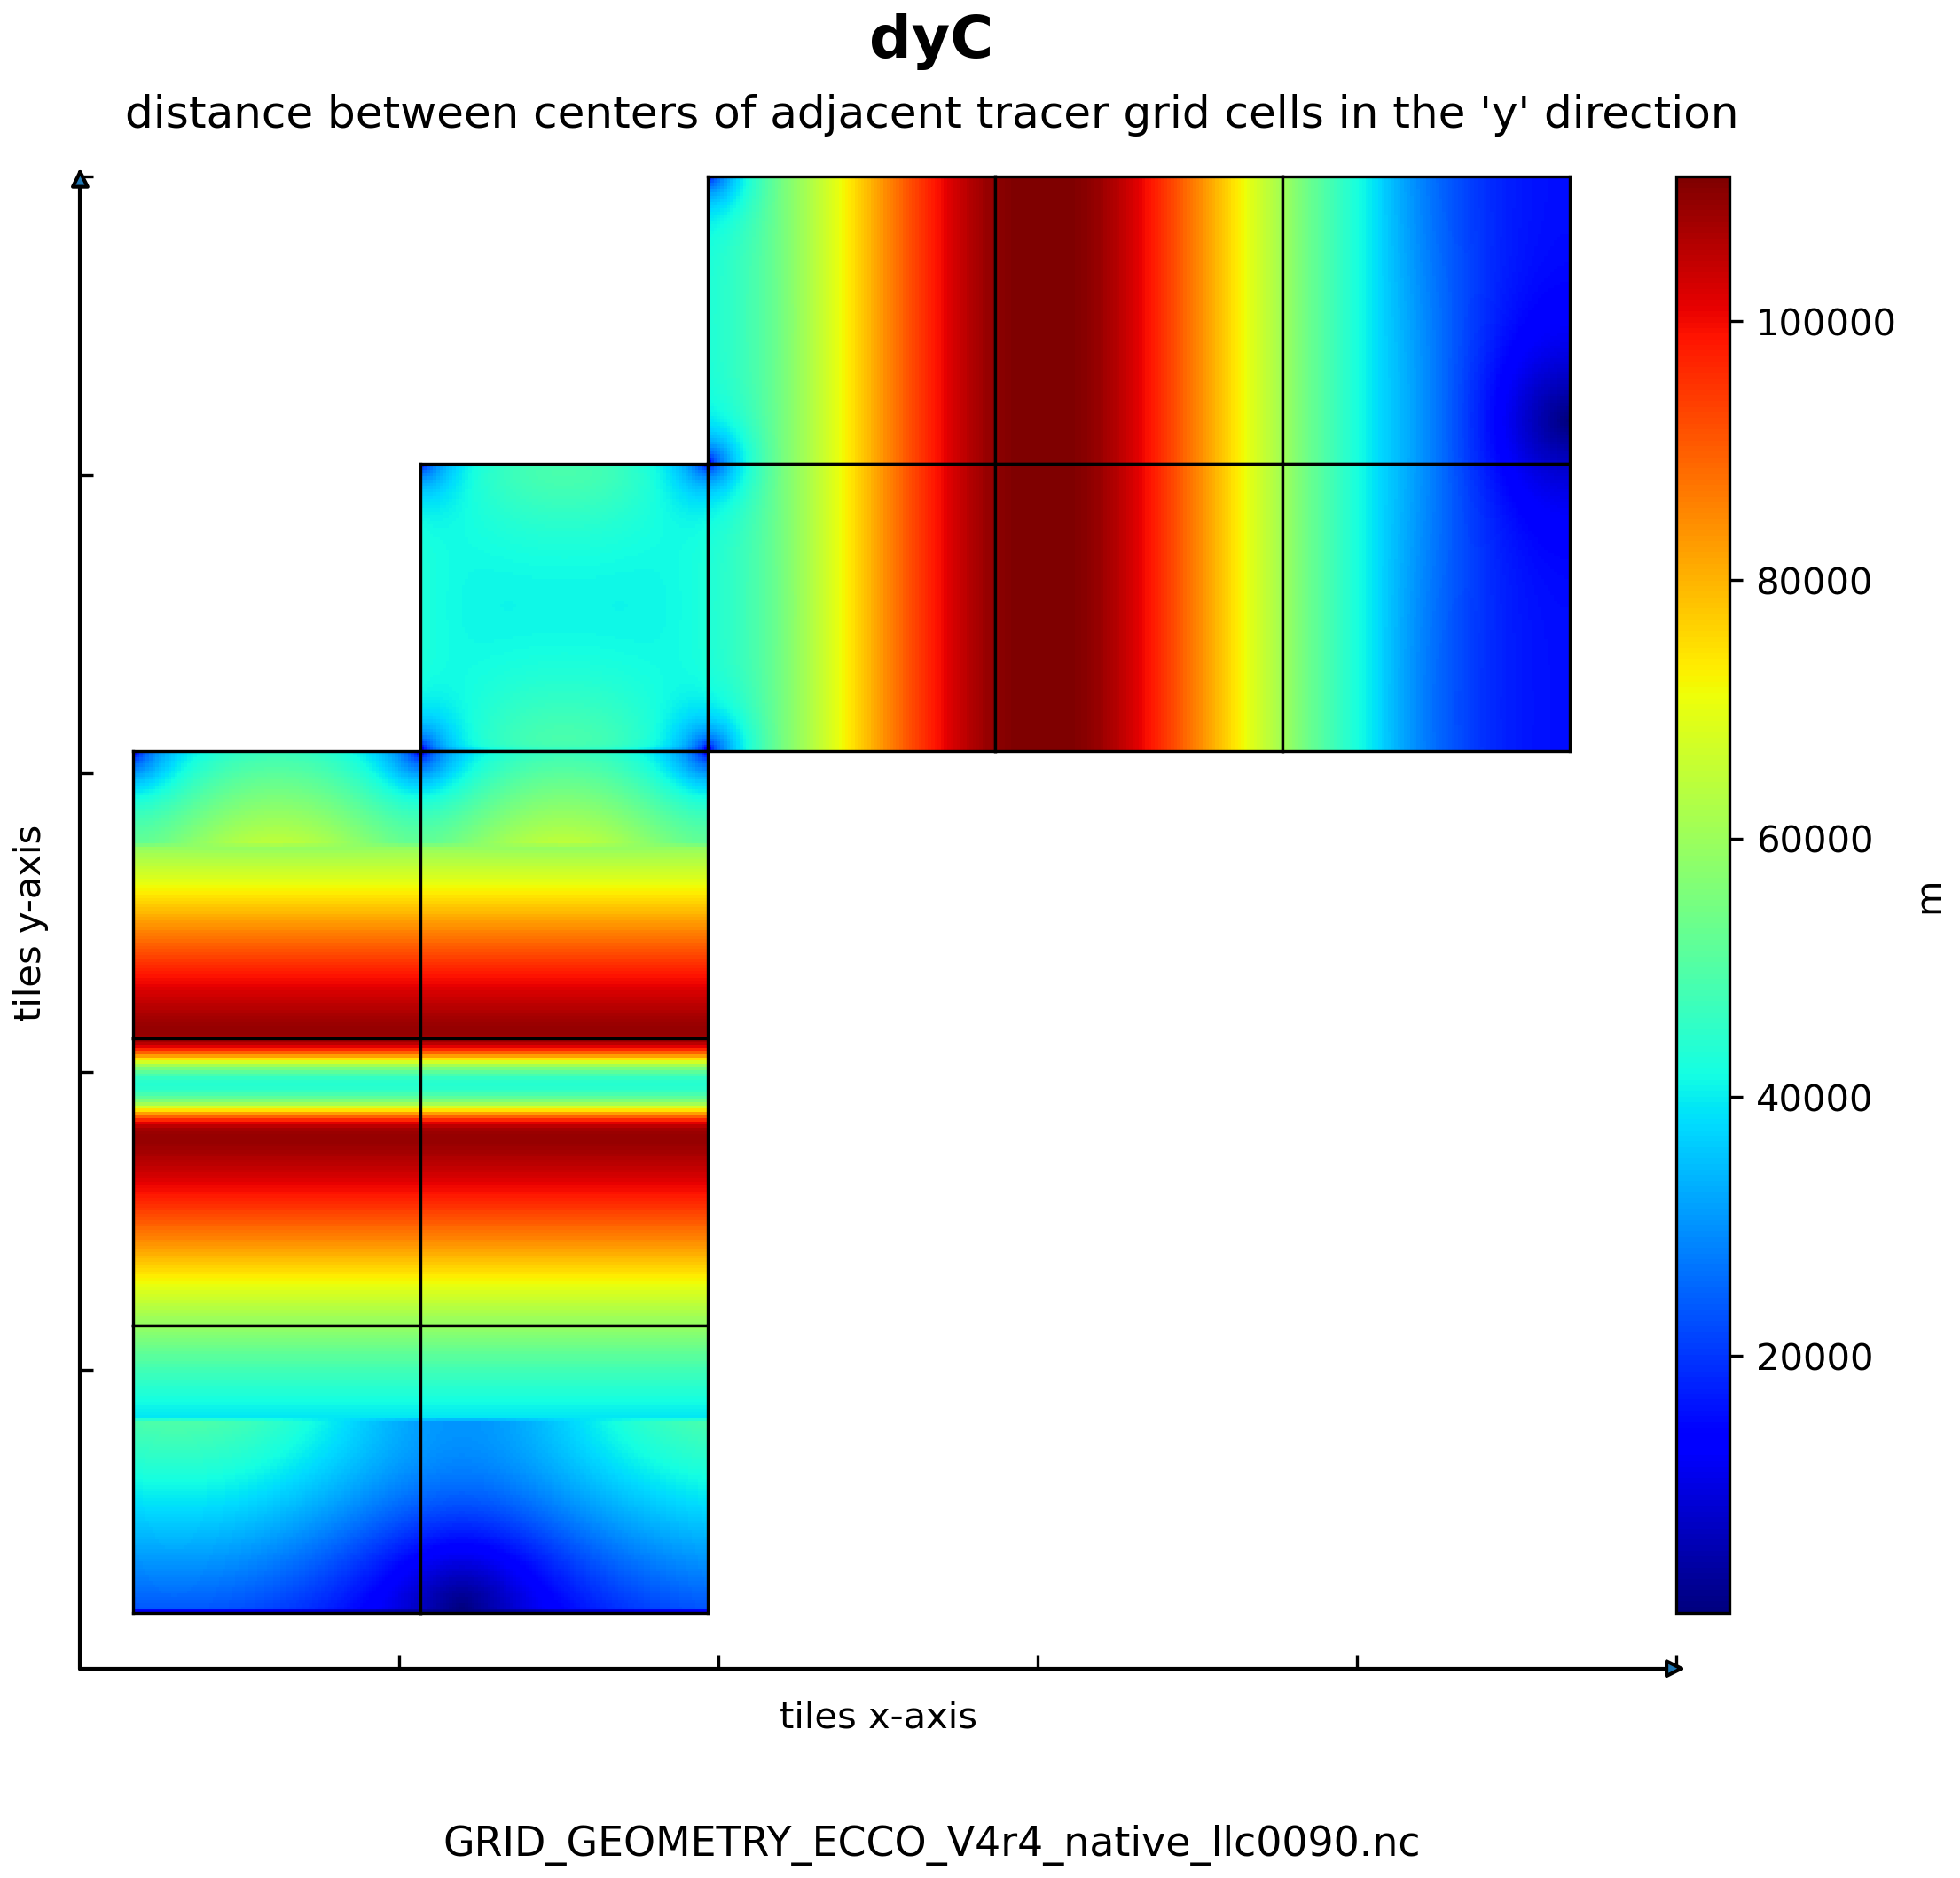
\includegraphics[scale=0.55]{../images/plots/native_plots_coords/Geometry_Parameters_for_the_Lat-Lon-Cap_90_(llc90)_Native_Model_Grid_(Version_4_Release_4)/dyC.png}
\caption{Dataset: GRID\_GEOMETRY\_ECCO, Variable: dyC}
\label{tab:table-GRID_GEOMETRY_ECCO_dyC-Plot}
\end{figure}
\pagebreak
\subsubsection{Native coordinates Variable: rAw}
\begin{longtable}{|m{0.06\textwidth}|m{0.3\textwidth}|m{0.45\textwidth}|m{0.11\textwidth}|}
\caption{Attributes description of the variable 'rAw' from GRID\_GEOMETRY\_ECCO's  dataset.}
\label{tab:table-GRID_GEOMETRY_ECCO_rAw} \\ 
\hline \endhead \hline \endfoot
\rowcolor{lightgray} \textbf{Storage Type} & \textbf{Variable Name} & \textbf{Description} & \textbf{Unit} \\ \hline
float32 & rAw & Area of 'v' grid cell & m2 \\ \hline
\multicolumn{4}{|c|}{\cellcolor{lightgray}{\textbf{Description of the variable in Common Data language (CDL)}}} \\ \hline
\multicolumn{4}{|c|}{\makecell{\parbox{.92\textwidth}{float32 rAw(tile, j, i\_g)\\
\hspace*{0.5cm}rAw: \_FillValue = 9.96921e+36\\
\hspace*{0.5cm}rAw: long\_name = "area of v grid cell"\\
\hspace*{0.5cm}rAw: units = m2\\
\hspace*{0.5cm}rAw: coordinate = YG XC\\
\hspace*{0.5cm}rAw: coverage\_content\_type = modelResult\\
\hspace*{0.5cm}rAw: standard\_name = cell\_area}}} \\ \hline
\rowcolor{lightgray} \multicolumn{4}{|c|}{\textbf{Comments}} \\ \hline
\multicolumn{4}{|p{1\textwidth}|}{Model 'v' grid cells are staggered in space between adjacent tracer grid cells in the 'x' direction. 'v' grid cell (i,j) is situated at the 'west' edge of tracer grid cell (i, j). note: 'west' does not correspond to geographic orientation but is used for convenience to describe the computational grid. see mitgcm documentation for details.} \\ \hline
\end{longtable}

\begin{figure}[H]
\centering
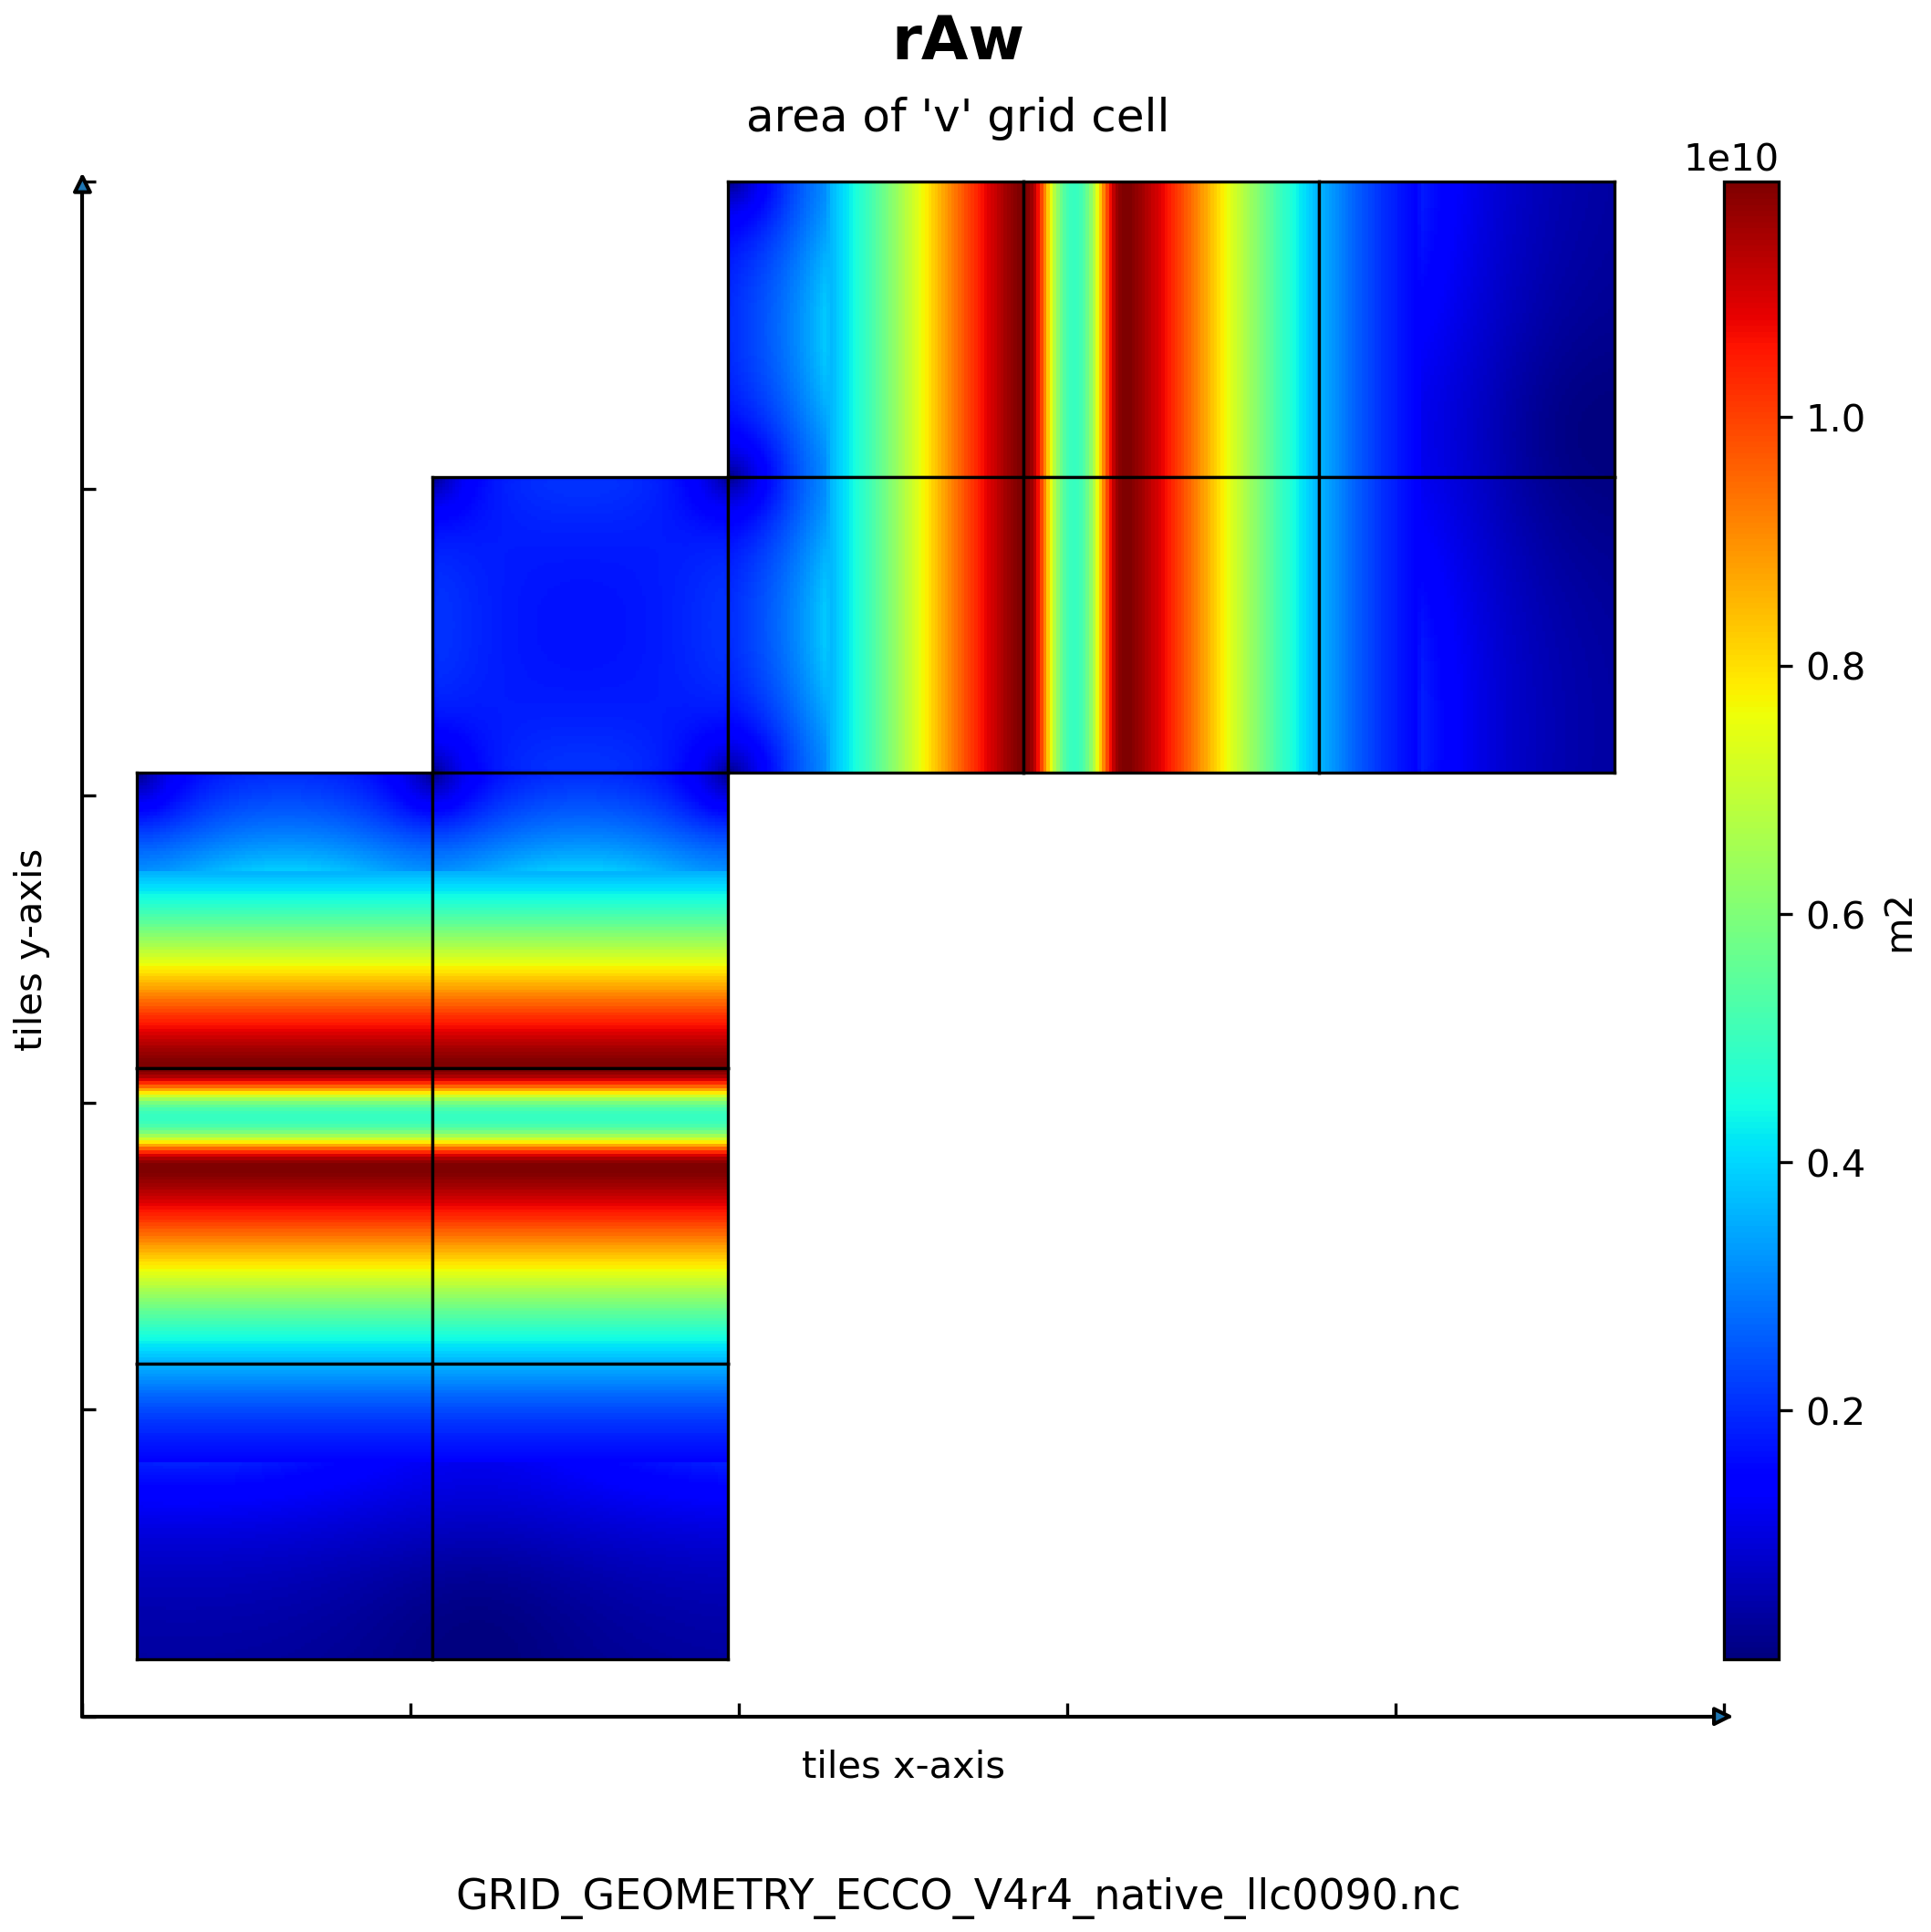
\includegraphics[scale=0.55]{../images/plots/native_plots_coords/Geometry_Parameters_for_the_Lat-Lon-Cap_90_(llc90)_Native_Model_Grid_(Version_4_Release_4)/rAw.png}
\caption{Dataset: GRID\_GEOMETRY\_ECCO, Variable: rAw}
\label{tab:table-GRID_GEOMETRY_ECCO_rAw-Plot}
\end{figure}
\pagebreak
\subsubsection{Native coordinates Variable: rAs}
\begin{longtable}{|m{0.06\textwidth}|m{0.3\textwidth}|m{0.45\textwidth}|m{0.11\textwidth}|}
\caption{Attributes description of the variable 'rAs' from GRID\_GEOMETRY\_ECCO's  dataset.}
\label{tab:table-GRID_GEOMETRY_ECCO_rAs} \\ 
\hline \endhead \hline \endfoot
\rowcolor{lightgray} \textbf{Storage Type} & \textbf{Variable Name} & \textbf{Description} & \textbf{Unit} \\ \hline
float32 & rAs & Area of 'u' grid cell & m2 \\ \hline
\multicolumn{4}{|c|}{\cellcolor{lightgray}{\textbf{Description of the variable in Common Data language (CDL)}}} \\ \hline
\multicolumn{4}{|c|}{\makecell{\parbox{.92\textwidth}{float32 rAs(tile, j\_g, i)\\
\hspace*{0.5cm}rAs: \_FillValue = 9.96921e+36\\
\hspace*{0.5cm}rAs: long\_name = "area of u grid cell"\\
\hspace*{0.5cm}rAs: units = m2\\
\hspace*{0.5cm}rAs: coordinates = YG XC\\
\hspace*{0.5cm}rAs: coverage\_content\_type = modelResult\\
\hspace*{0.5cm}rAs: standard\_name = cell\_area}}} \\ \hline
\rowcolor{lightgray} \multicolumn{4}{|c|}{\textbf{Comments}} \\ \hline
\multicolumn{4}{|p{1\textwidth}|}{Model 'u' grid cells are staggered in space between adjacent tracer grid cells in the 'y' direction. 'u' grid cell (i,j) is situated at the 'south' edge of tracer grid cell (i, j). note: 'south' does not correspond to geographic orientation but is used for convenience to describe the computational grid. see mitgcm documentation for details.} \\ \hline
\end{longtable}

\begin{figure}[H]
\centering
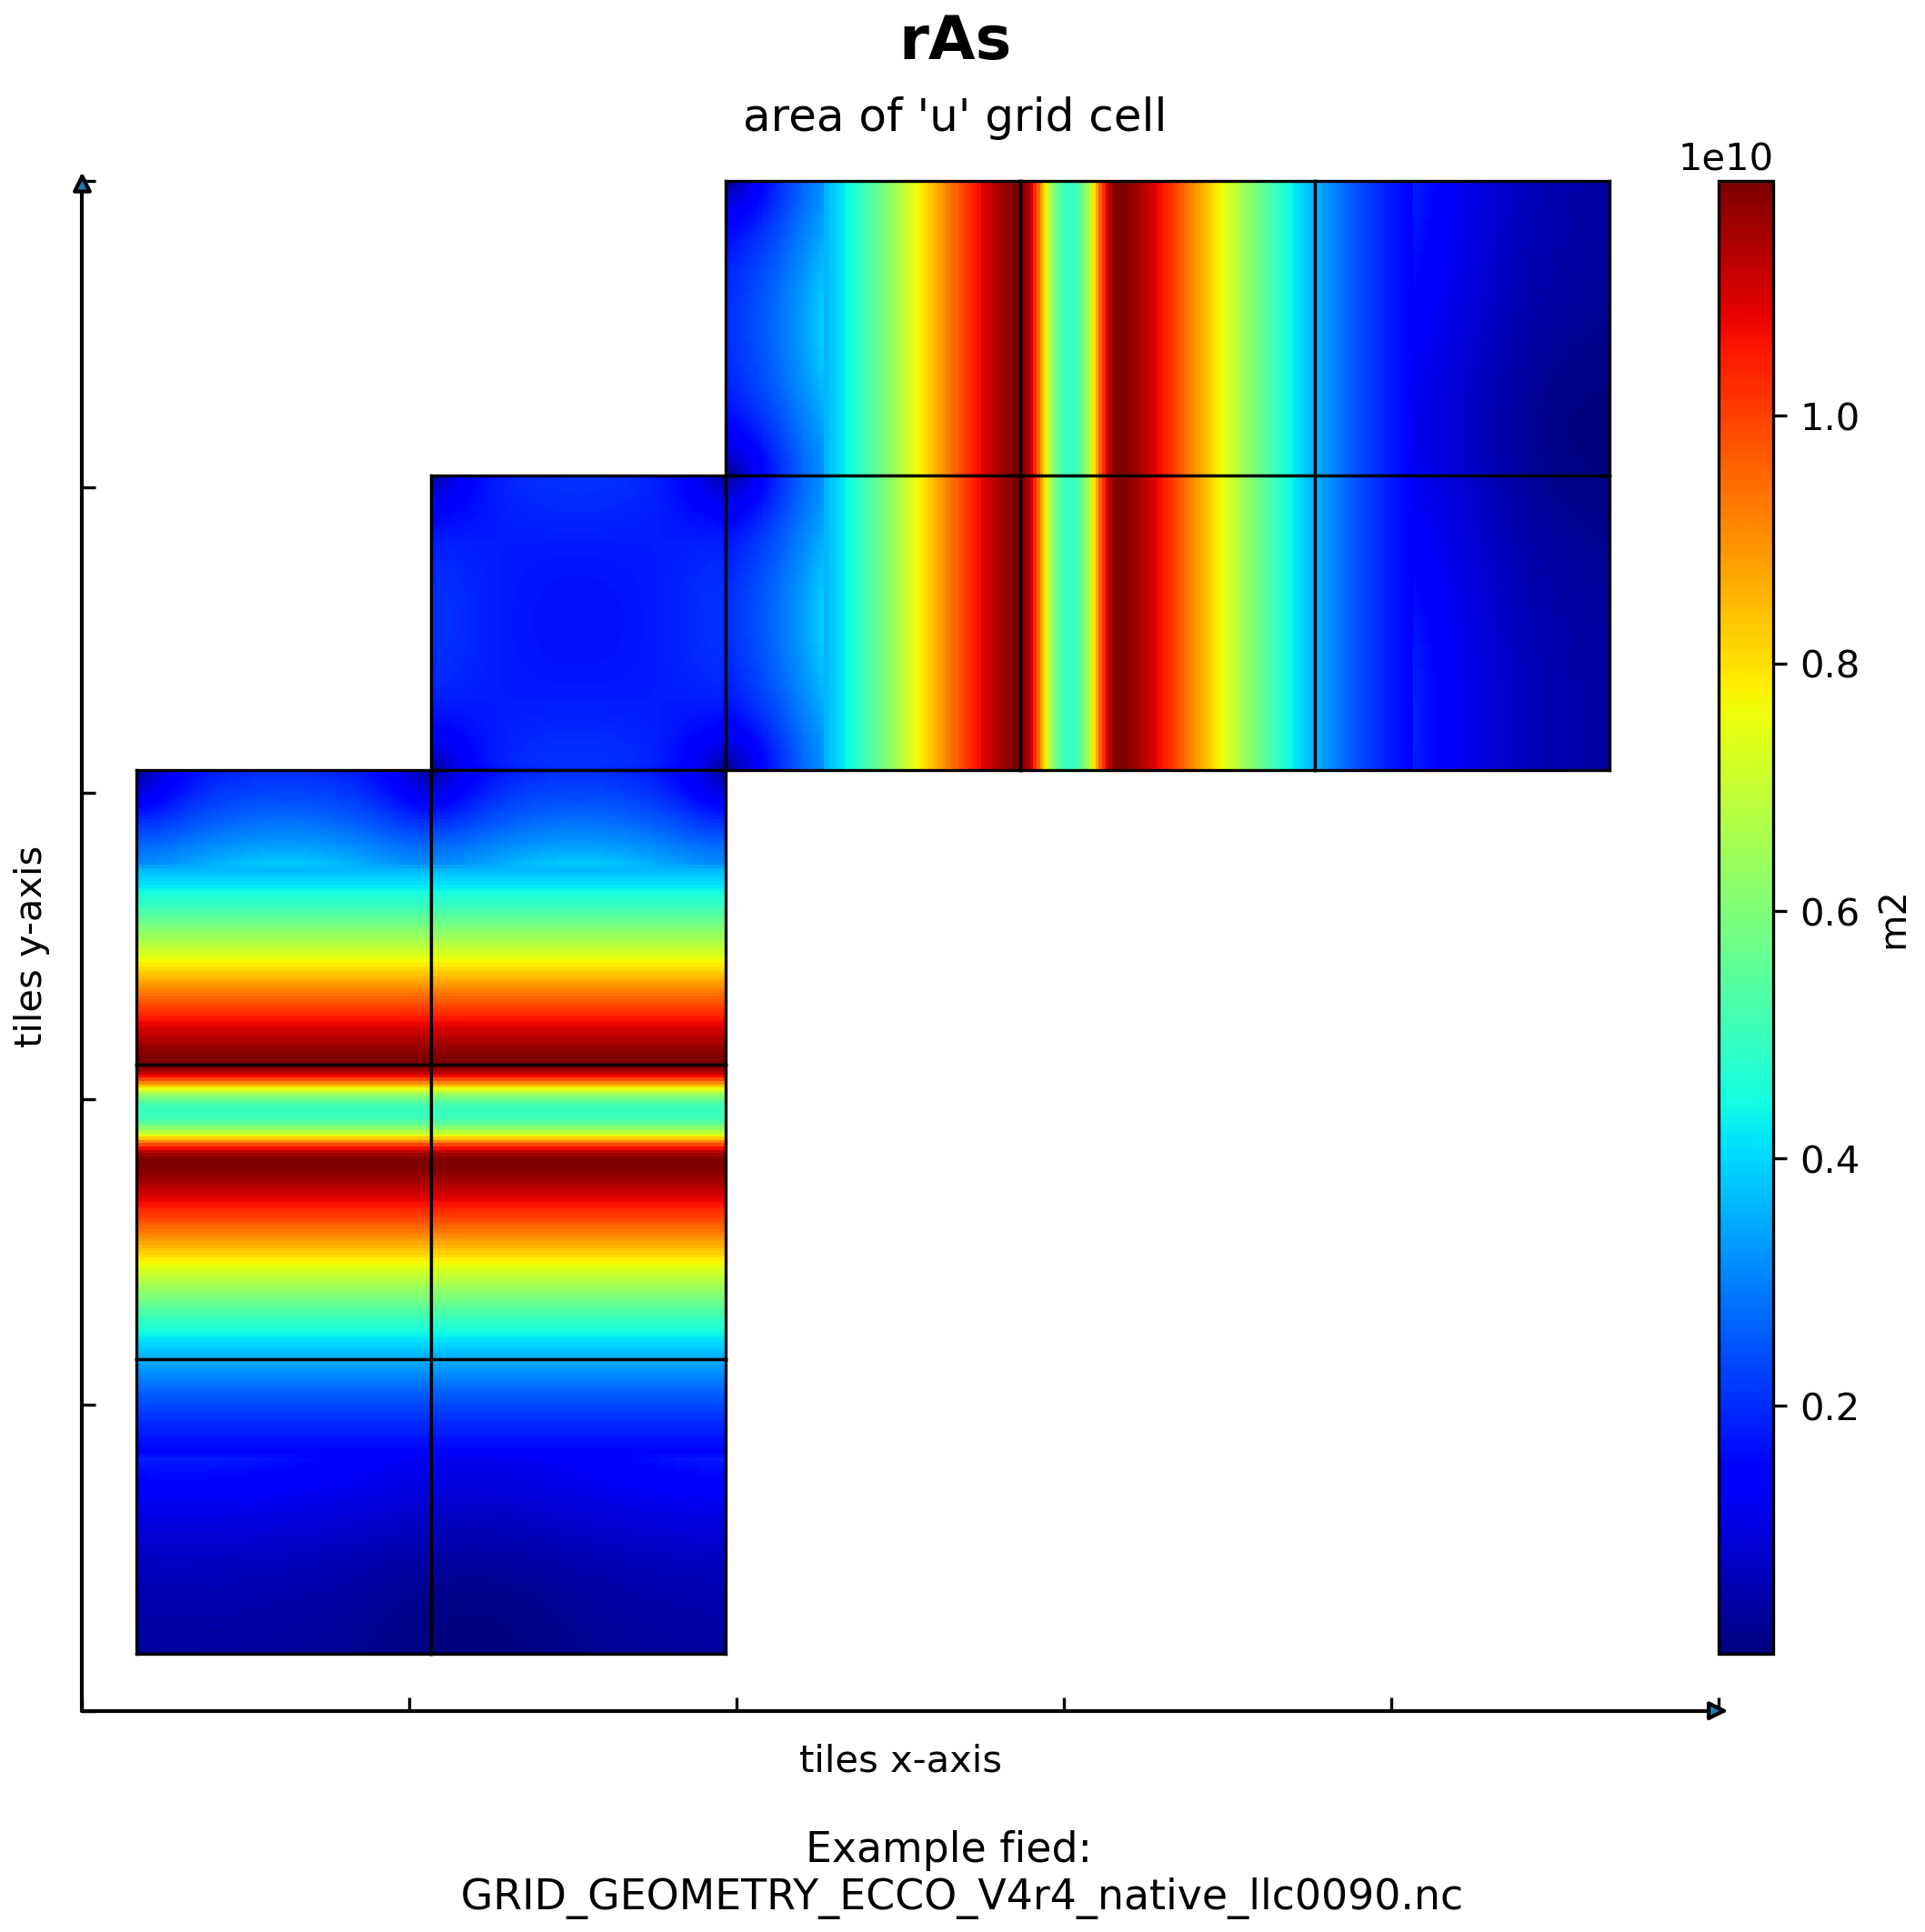
\includegraphics[scale=0.55]{../images/plots/native_plots_coords/Geometry_Parameters_for_the_Lat-Lon-Cap_90_(llc90)_Native_Model_Grid_(Version_4_Release_4)/rAs.png}
\caption{Dataset: GRID\_GEOMETRY\_ECCO, Variable: rAs}
\label{tab:table-GRID_GEOMETRY_ECCO_rAs-Plot}
\end{figure}
\pagebreak
\subsubsection{Native coordinates Variable: hFacC}
\begin{longtable}{|m{0.06\textwidth}|m{0.3\textwidth}|m{0.45\textwidth}|m{0.11\textwidth}|}
\caption{Attributes description of the variable 'hFacC' from GRID\_GEOMETRY\_ECCO's  dataset.}
\label{tab:table-GRID_GEOMETRY_ECCO_hFacC} \\ 
\hline \endhead \hline \endfoot
\rowcolor{lightgray} \textbf{Storage Type} & \textbf{Variable Name} & \textbf{Description} & \textbf{Unit} \\ \hline
float32 & hFacC & Vertical open fraction of tracer grid cell & 1 \\ \hline
\multicolumn{4}{|c|}{\cellcolor{lightgray}{\textbf{Description of the variable in Common Data language (CDL)}}} \\ \hline
\multicolumn{4}{|c|}{\makecell{\parbox{.92\textwidth}{float32 hFacC(k, tile, j, i)\\
\hspace*{0.5cm}hFacC: \_FillValue = 9.96921e+36\\
\hspace*{0.5cm}hFacC: long\_name = vertical open fraction of tracer grid cell\\
\hspace*{0.5cm}hFacC: coverage\_content\_type = modelResult\\
\hspace*{0.5cm}hFacC: units = 1\\
\hspace*{0.5cm}hFacC: coordinates = Z YC XC}}} \\ \hline
\rowcolor{lightgray} \multicolumn{4}{|c|}{\textbf{Comments}} \\ \hline
\multicolumn{4}{|p{1\textwidth}|}{Tracer grid cells may be fractionally closed in the vertical. the open vertical fraction is hfacc. the model allows for partially-filled cells to represent topographic variations more smoothly (hfacc < 1). completely closed (dry) tracer grid cells have hfacc = 0. note: the model z* coordinate system allows hfacc to vary through time. a time-invariant hfacc field is provided for reference.} \\ \hline
\end{longtable}

\begin{figure}[H]
\centering
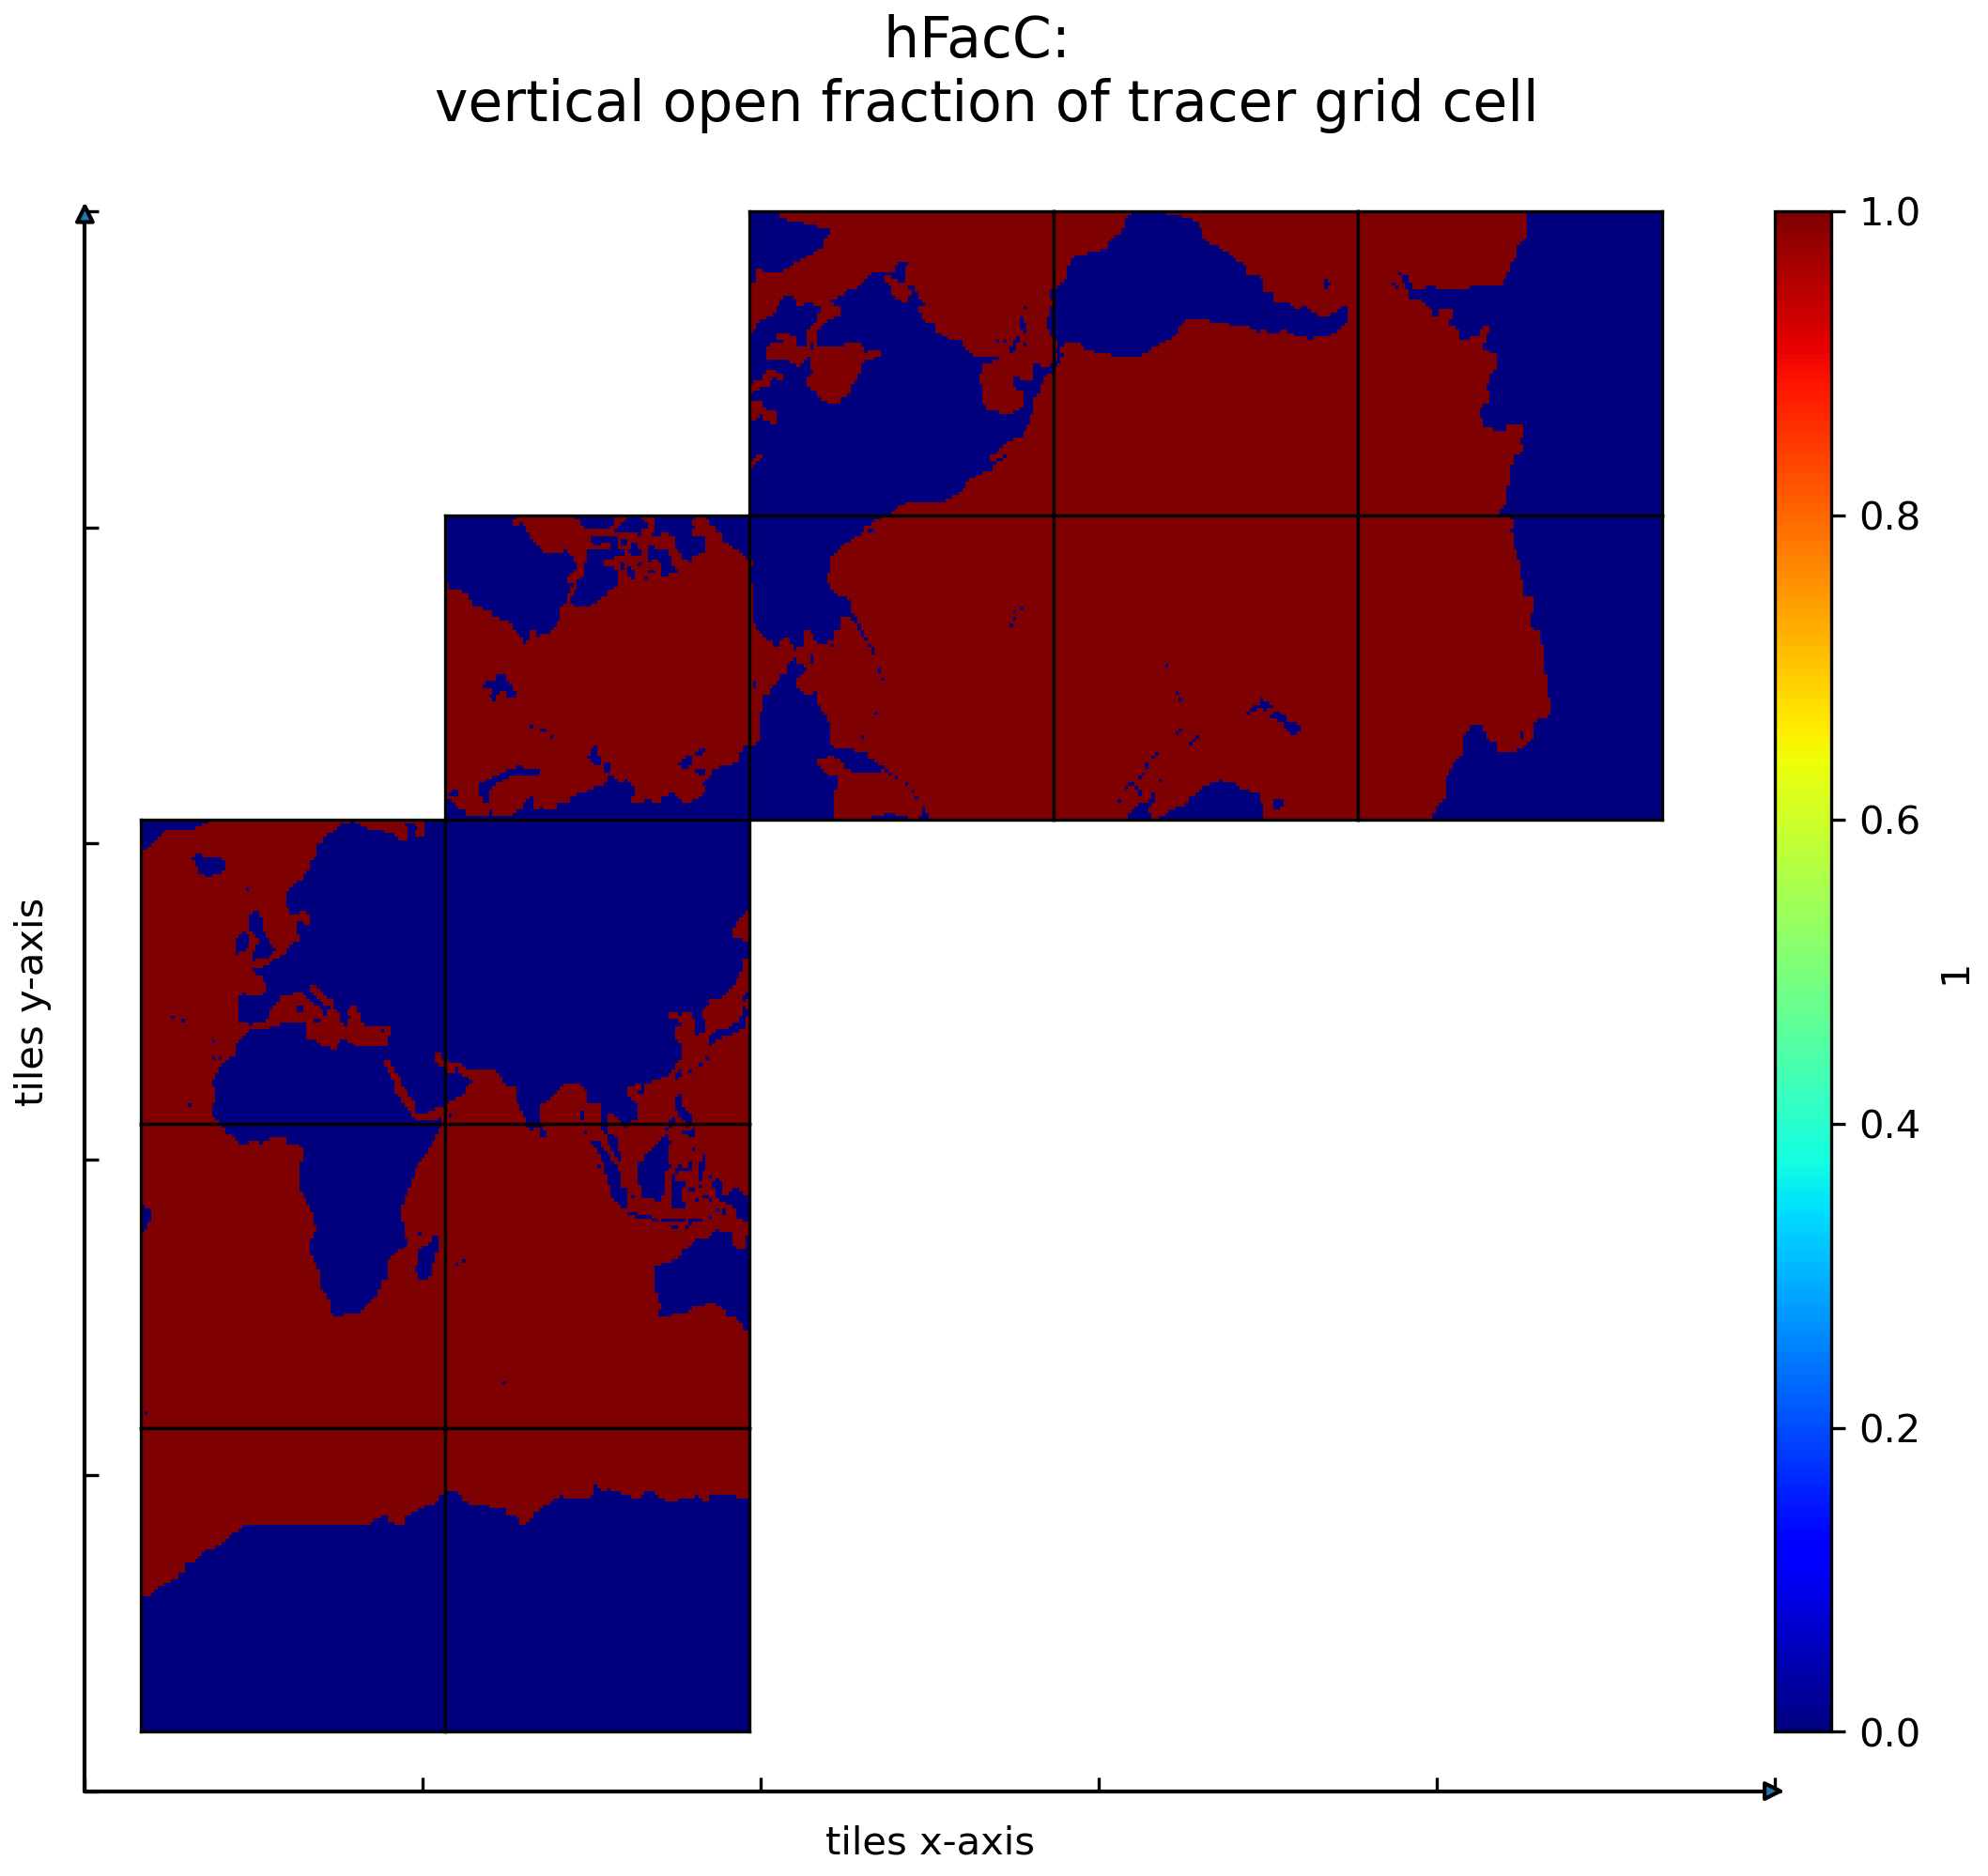
\includegraphics[scale=0.55]{../images/plots/native_plots_coords/Geometry_Parameters_for_the_Lat-Lon-Cap_90_(llc90)_Native_Model_Grid_(Version_4_Release_4)/hFacC.png}
\caption{Dataset: GRID\_GEOMETRY\_ECCO, Variable: hFacC}
\label{tab:table-GRID_GEOMETRY_ECCO_hFacC-Plot}
\end{figure}
\pagebreak
\subsubsection{Native coordinates Variable: hFacW}
\begin{longtable}{|m{0.06\textwidth}|m{0.3\textwidth}|m{0.45\textwidth}|m{0.11\textwidth}|}
\caption{Attributes description of the variable 'hFacW' from GRID\_GEOMETRY\_ECCO's  dataset.}
\label{tab:table-GRID_GEOMETRY_ECCO_hFacW} \\ 
\hline \endhead \hline \endfoot
\rowcolor{lightgray} \textbf{Storage Type} & \textbf{Variable Name} & \textbf{Description} & \textbf{Unit} \\ \hline
float32 & hFacW & Vertical open fraction of tracer grid cell 'west' face & 1 \\ \hline
\multicolumn{4}{|c|}{\cellcolor{lightgray}{\textbf{Description of the variable in Common Data language (CDL)}}} \\ \hline
\multicolumn{4}{|c|}{\makecell{\parbox{.92\textwidth}{float32 hFacW(k, tile, j, i\_g)\\
\hspace*{0.5cm}hFacW: \_FillValue = 9.96921e+36\\
\hspace*{0.5cm}hFacW: long\_name = "vertical open fraction of tracer grid cell west face"\\
\hspace*{0.5cm}hFacW: coverage\_content\_type = modelResult\\
\hspace*{0.5cm}hFacW: units = 1\\
\hspace*{0.5cm}hFacW: coordinates = Z}}} \\ \hline
\rowcolor{lightgray} \multicolumn{4}{|c|}{\textbf{Comments}} \\ \hline
\multicolumn{4}{|p{1\textwidth}|}{The 'west' face of tracer grid cells may be fractionally closed in the vertical. the open vertical fraction is hfacw. the model allows for partially-filled cells for smoother representation of seafloor topography. tracer grid cells adjacent in the 'x' direction that are partially closed in the vertical have hfacw < 1. the model z* coordinate system used by the model permits hfacc, and therefore hfacw, to vary through time. a time-invariant hfacw field is provided for reference. note: the term 'west' does not correspond to geographic orientation but is used for convenience to describe the computational grid. see mitgcm documentation for details.} \\ \hline
\end{longtable}

\begin{figure}[H]
\centering
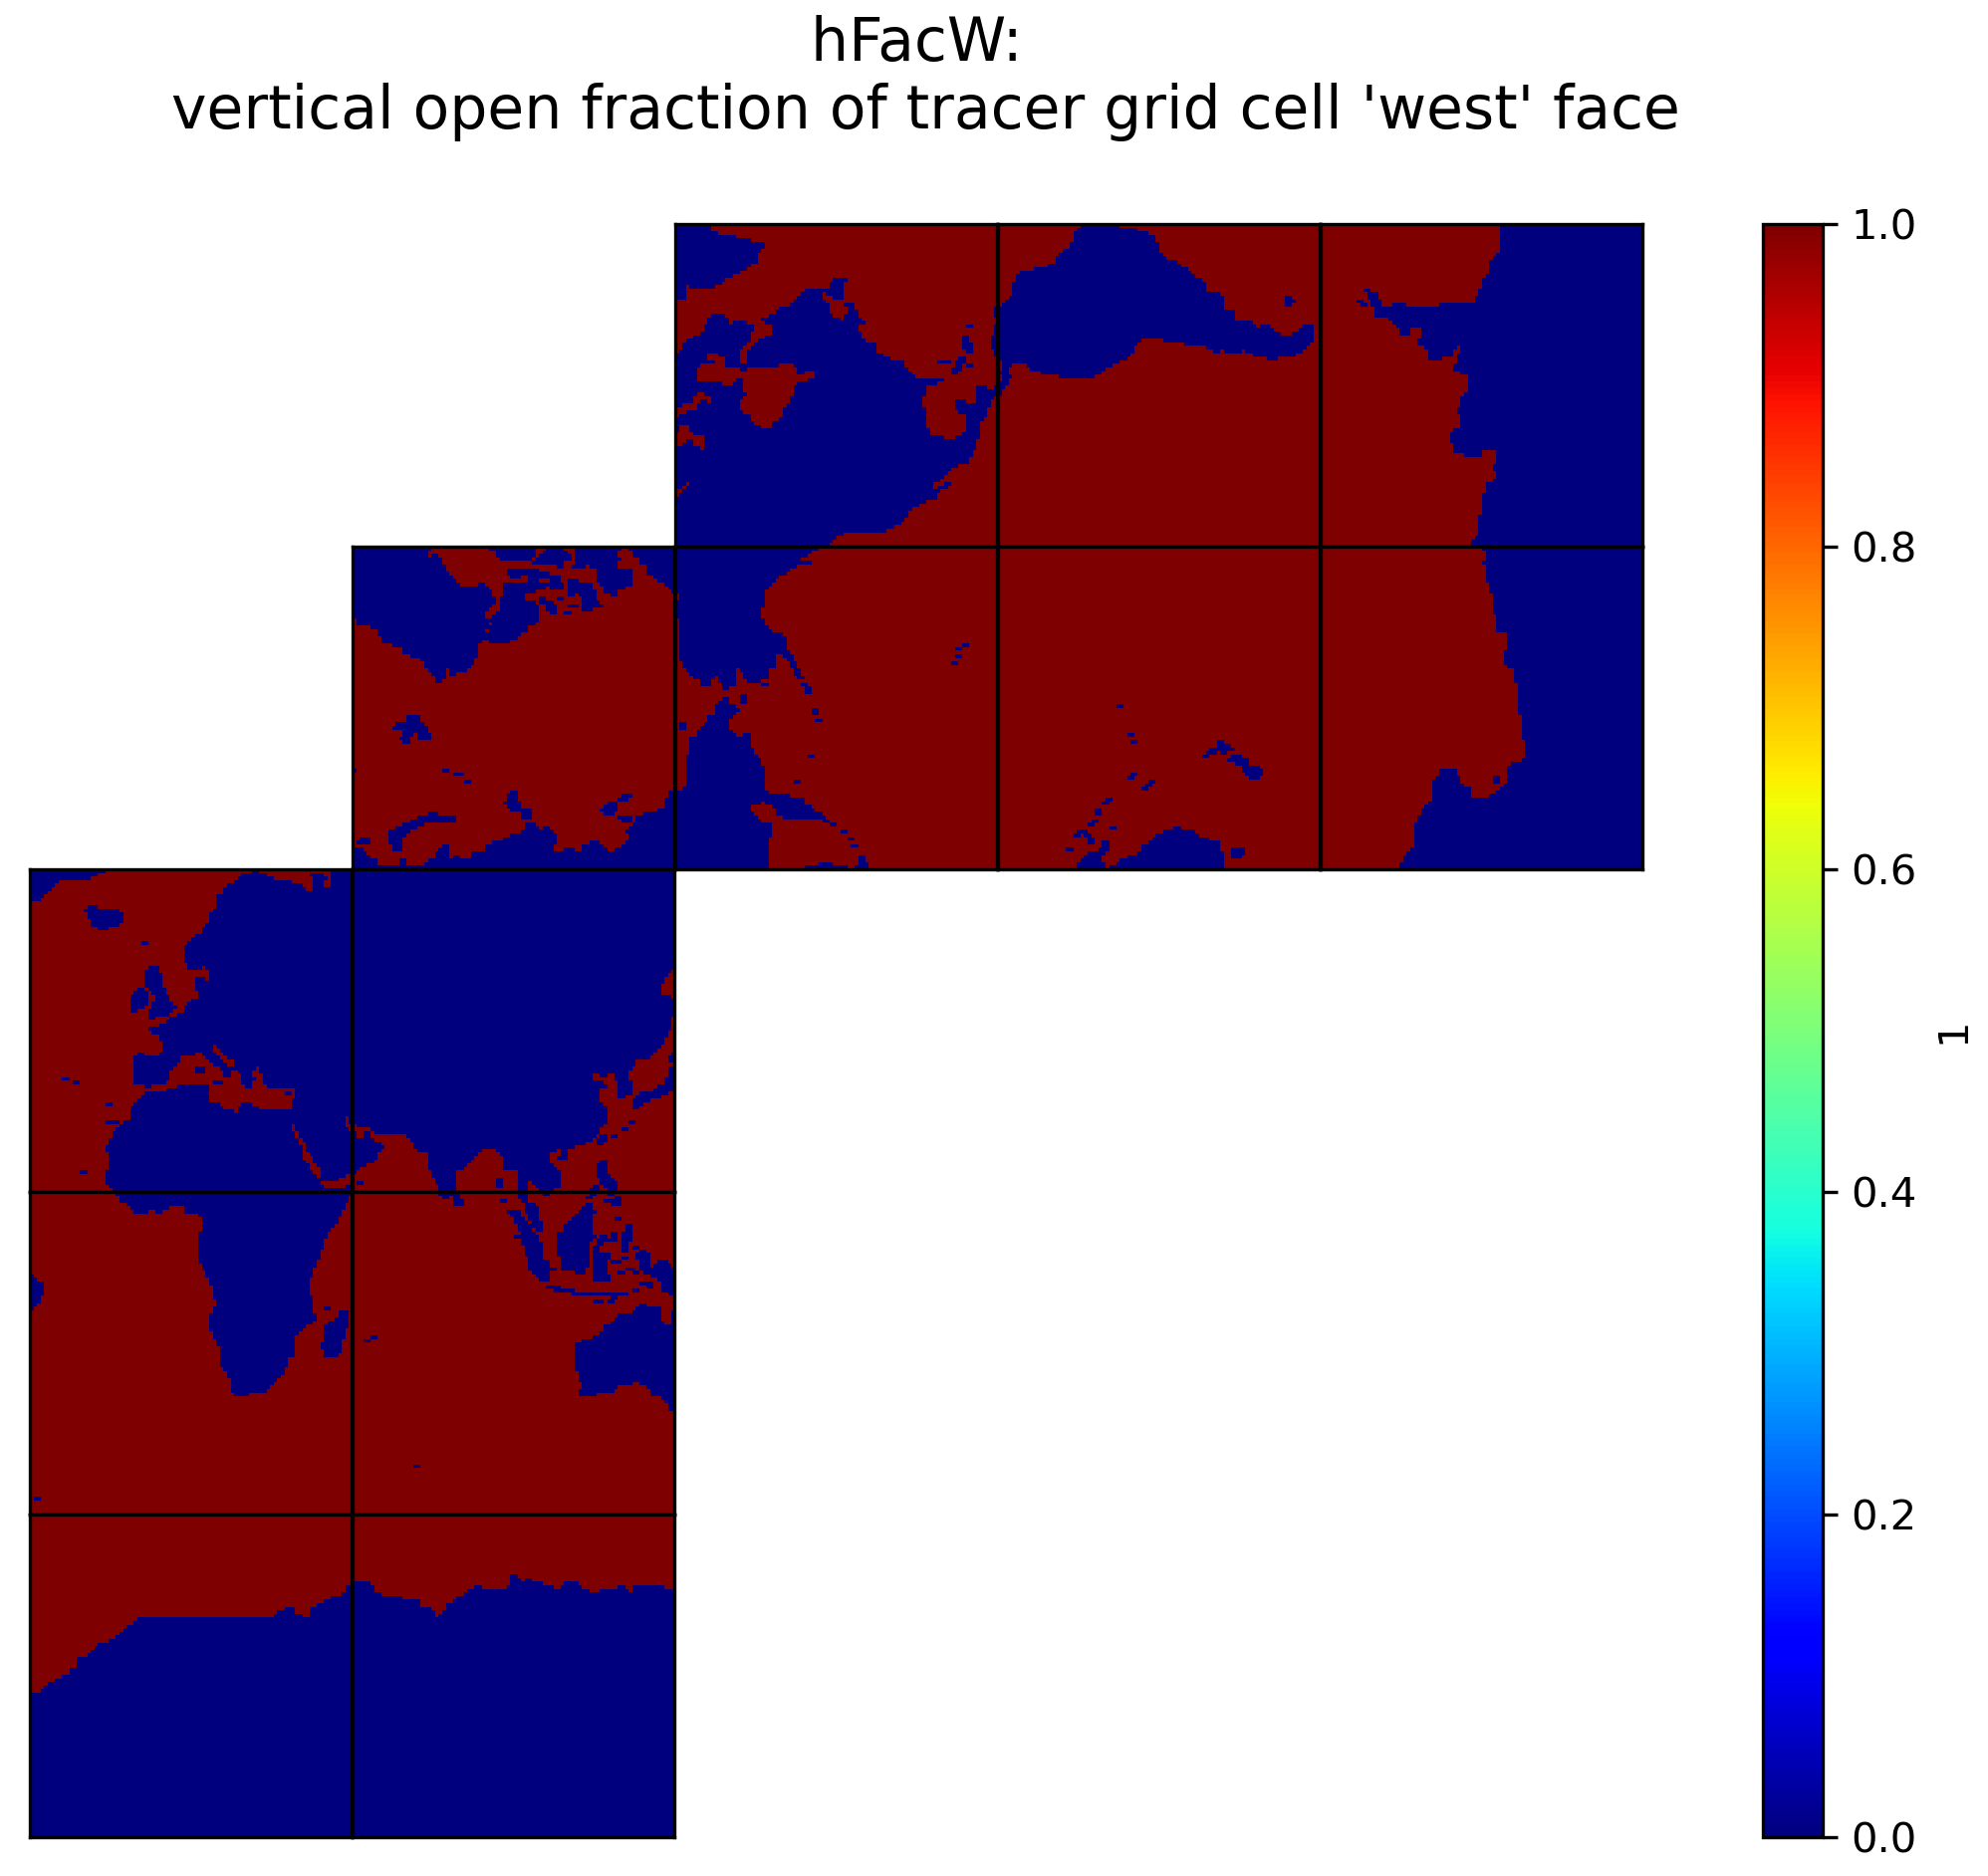
\includegraphics[scale=0.55]{../images/plots/native_plots_coords/Geometry_Parameters_for_the_Lat-Lon-Cap_90_(llc90)_Native_Model_Grid_(Version_4_Release_4)/hFacW.png}
\caption{Dataset: GRID\_GEOMETRY\_ECCO, Variable: hFacW}
\label{tab:table-GRID_GEOMETRY_ECCO_hFacW-Plot}
\end{figure}
\pagebreak
\subsubsection{Native coordinates Variable: hFacS}
\begin{longtable}{|m{0.06\textwidth}|m{0.3\textwidth}|m{0.45\textwidth}|m{0.11\textwidth}|}
\caption{Attributes description of the variable 'hFacS' from GRID\_GEOMETRY\_ECCO's  dataset.}
\label{tab:table-GRID_GEOMETRY_ECCO_hFacS} \\ 
\hline \endhead \hline \endfoot
\rowcolor{lightgray} \textbf{Storage Type} & \textbf{Variable Name} & \textbf{Description} & \textbf{Unit} \\ \hline
float32 & hFacS & Vertical open fraction of tracer grid cell 'south' face & 1 \\ \hline
\multicolumn{4}{|c|}{\cellcolor{lightgray}{\textbf{Description of the variable in Common Data language (CDL)}}} \\ \hline
\multicolumn{4}{|c|}{\makecell{\parbox{.92\textwidth}{float32 hFacS(k, tile, j\_g, i)\\
\hspace*{0.5cm}hFacS: \_FillValue = 9.96921e+36\\
\hspace*{0.5cm}hFacS: long\_name = "vertical open fraction of tracer grid cell south face"\\
\hspace*{0.5cm}hFacS: coverage\_content\_type = modelResult\\
\hspace*{0.5cm}hFacS: units = 1\\
\hspace*{0.5cm}hFacS: coordinates = Z}}} \\ \hline
\rowcolor{lightgray} \multicolumn{4}{|c|}{\textbf{Comments}} \\ \hline
\multicolumn{4}{|p{1\textwidth}|}{The 'south' face of tracer grid cells may be fractionally closed in the vertical. the open vertical fraction is hfacs. the model allows for partially-filled cells for smoother representation of seafloor topography. tracer grid cells adjacent in the 'y' direction that are partially closed in the vertical have hfacs < 1. the model z* coordinate system used by the model permits hfacc, and therefore hfacs, to vary through time. a time-invariant hfacs field is provided for reference. note:  the term 'south' does not correspond to geographic orientation but is used for convenience to describe the computational grid. see mitgcm documentation for details.} \\ \hline
\end{longtable}

\begin{figure}[H]
\centering
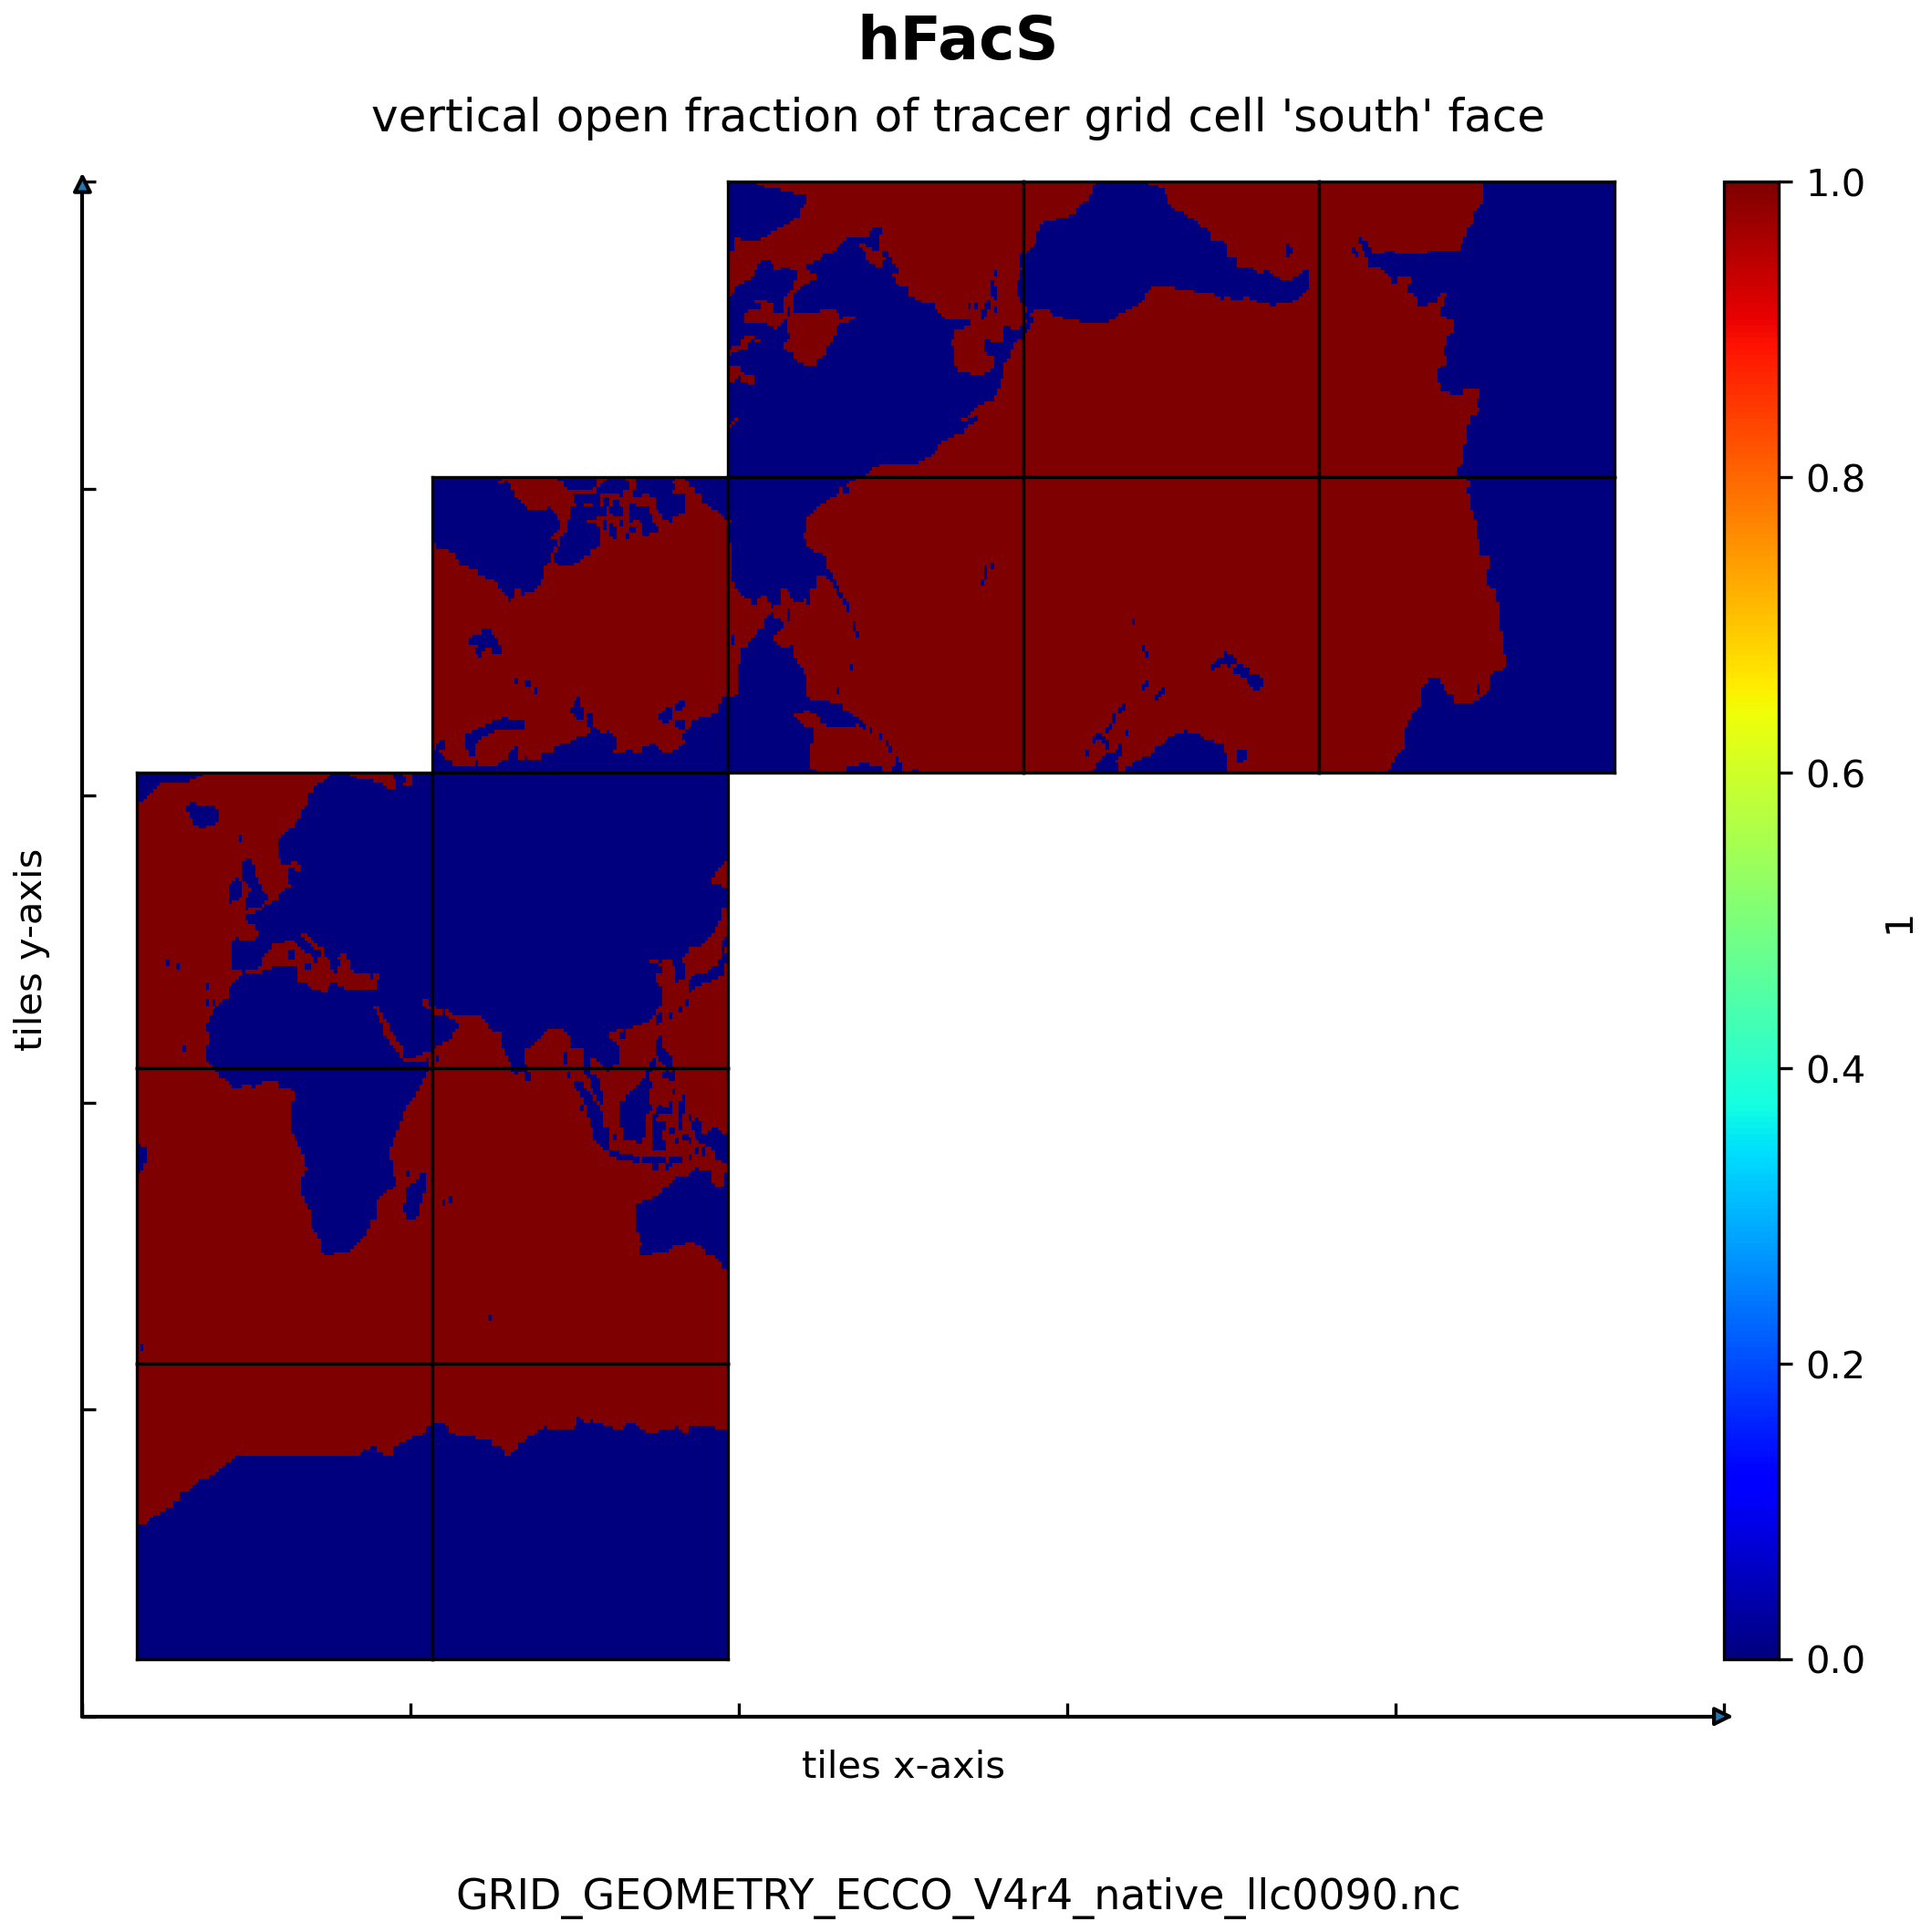
\includegraphics[scale=0.55]{../images/plots/native_plots_coords/Geometry_Parameters_for_the_Lat-Lon-Cap_90_(llc90)_Native_Model_Grid_(Version_4_Release_4)/hFacS.png}
\caption{Dataset: GRID\_GEOMETRY\_ECCO, Variable: hFacS}
\label{tab:table-GRID_GEOMETRY_ECCO_hFacS-Plot}
\end{figure}
\pagebreak
\subsubsection{Native coordinates Variable: maskC}
\begin{longtable}{|m{0.06\textwidth}|m{0.3\textwidth}|m{0.45\textwidth}|m{0.11\textwidth}|}
\caption{Attributes description of the variable 'maskC' from GRID\_GEOMETRY\_ECCO's  dataset.}
\label{tab:table-GRID_GEOMETRY_ECCO_maskC} \\ 
\hline \endhead \hline \endfoot
\rowcolor{lightgray} \textbf{Storage Type} & \textbf{Variable Name} & \textbf{Description} & \textbf{Unit} \\ \hline
bool & maskC & Wet/dry boolean mask for tracer grid cell & N/A \\ \hline
\multicolumn{4}{|c|}{\cellcolor{lightgray}{\textbf{Description of the variable in Common Data language (CDL)}}} \\ \hline
\multicolumn{4}{|c|}{\makecell{\parbox{.92\textwidth}{bool maskC(k, tile, j, i)\\
\hspace*{0.5cm}maskC: \_FillValue = 1\\
\hspace*{0.5cm}maskC: long\_name = wet/dry boolean mask for tracer grid cell\\
\hspace*{0.5cm}maskC: coverage\_content\_type = modelResult\\
\hspace*{0.5cm}maskC: coordinates = Z YC XC}}} \\ \hline
\rowcolor{lightgray} \multicolumn{4}{|c|}{\textbf{Comments}} \\ \hline
\multicolumn{4}{|p{1\textwidth}|}{True for tracer grid cells with nonzero open vertical fraction (hfacc > 0), otherwise false. although hfacc can vary though time, cells will never close if starting open and will never open if starting closed: hfacc(i,j,k,t) > 0 for all t, if hfacc(i,j,k,t=0) and hfacc(i,j,k,t) = 0 for all t, if hfacc(i,j,k,t=0) = 0. therefore, maskc is time invariant.} \\ \hline
\end{longtable}

\begin{figure}[H]
\centering
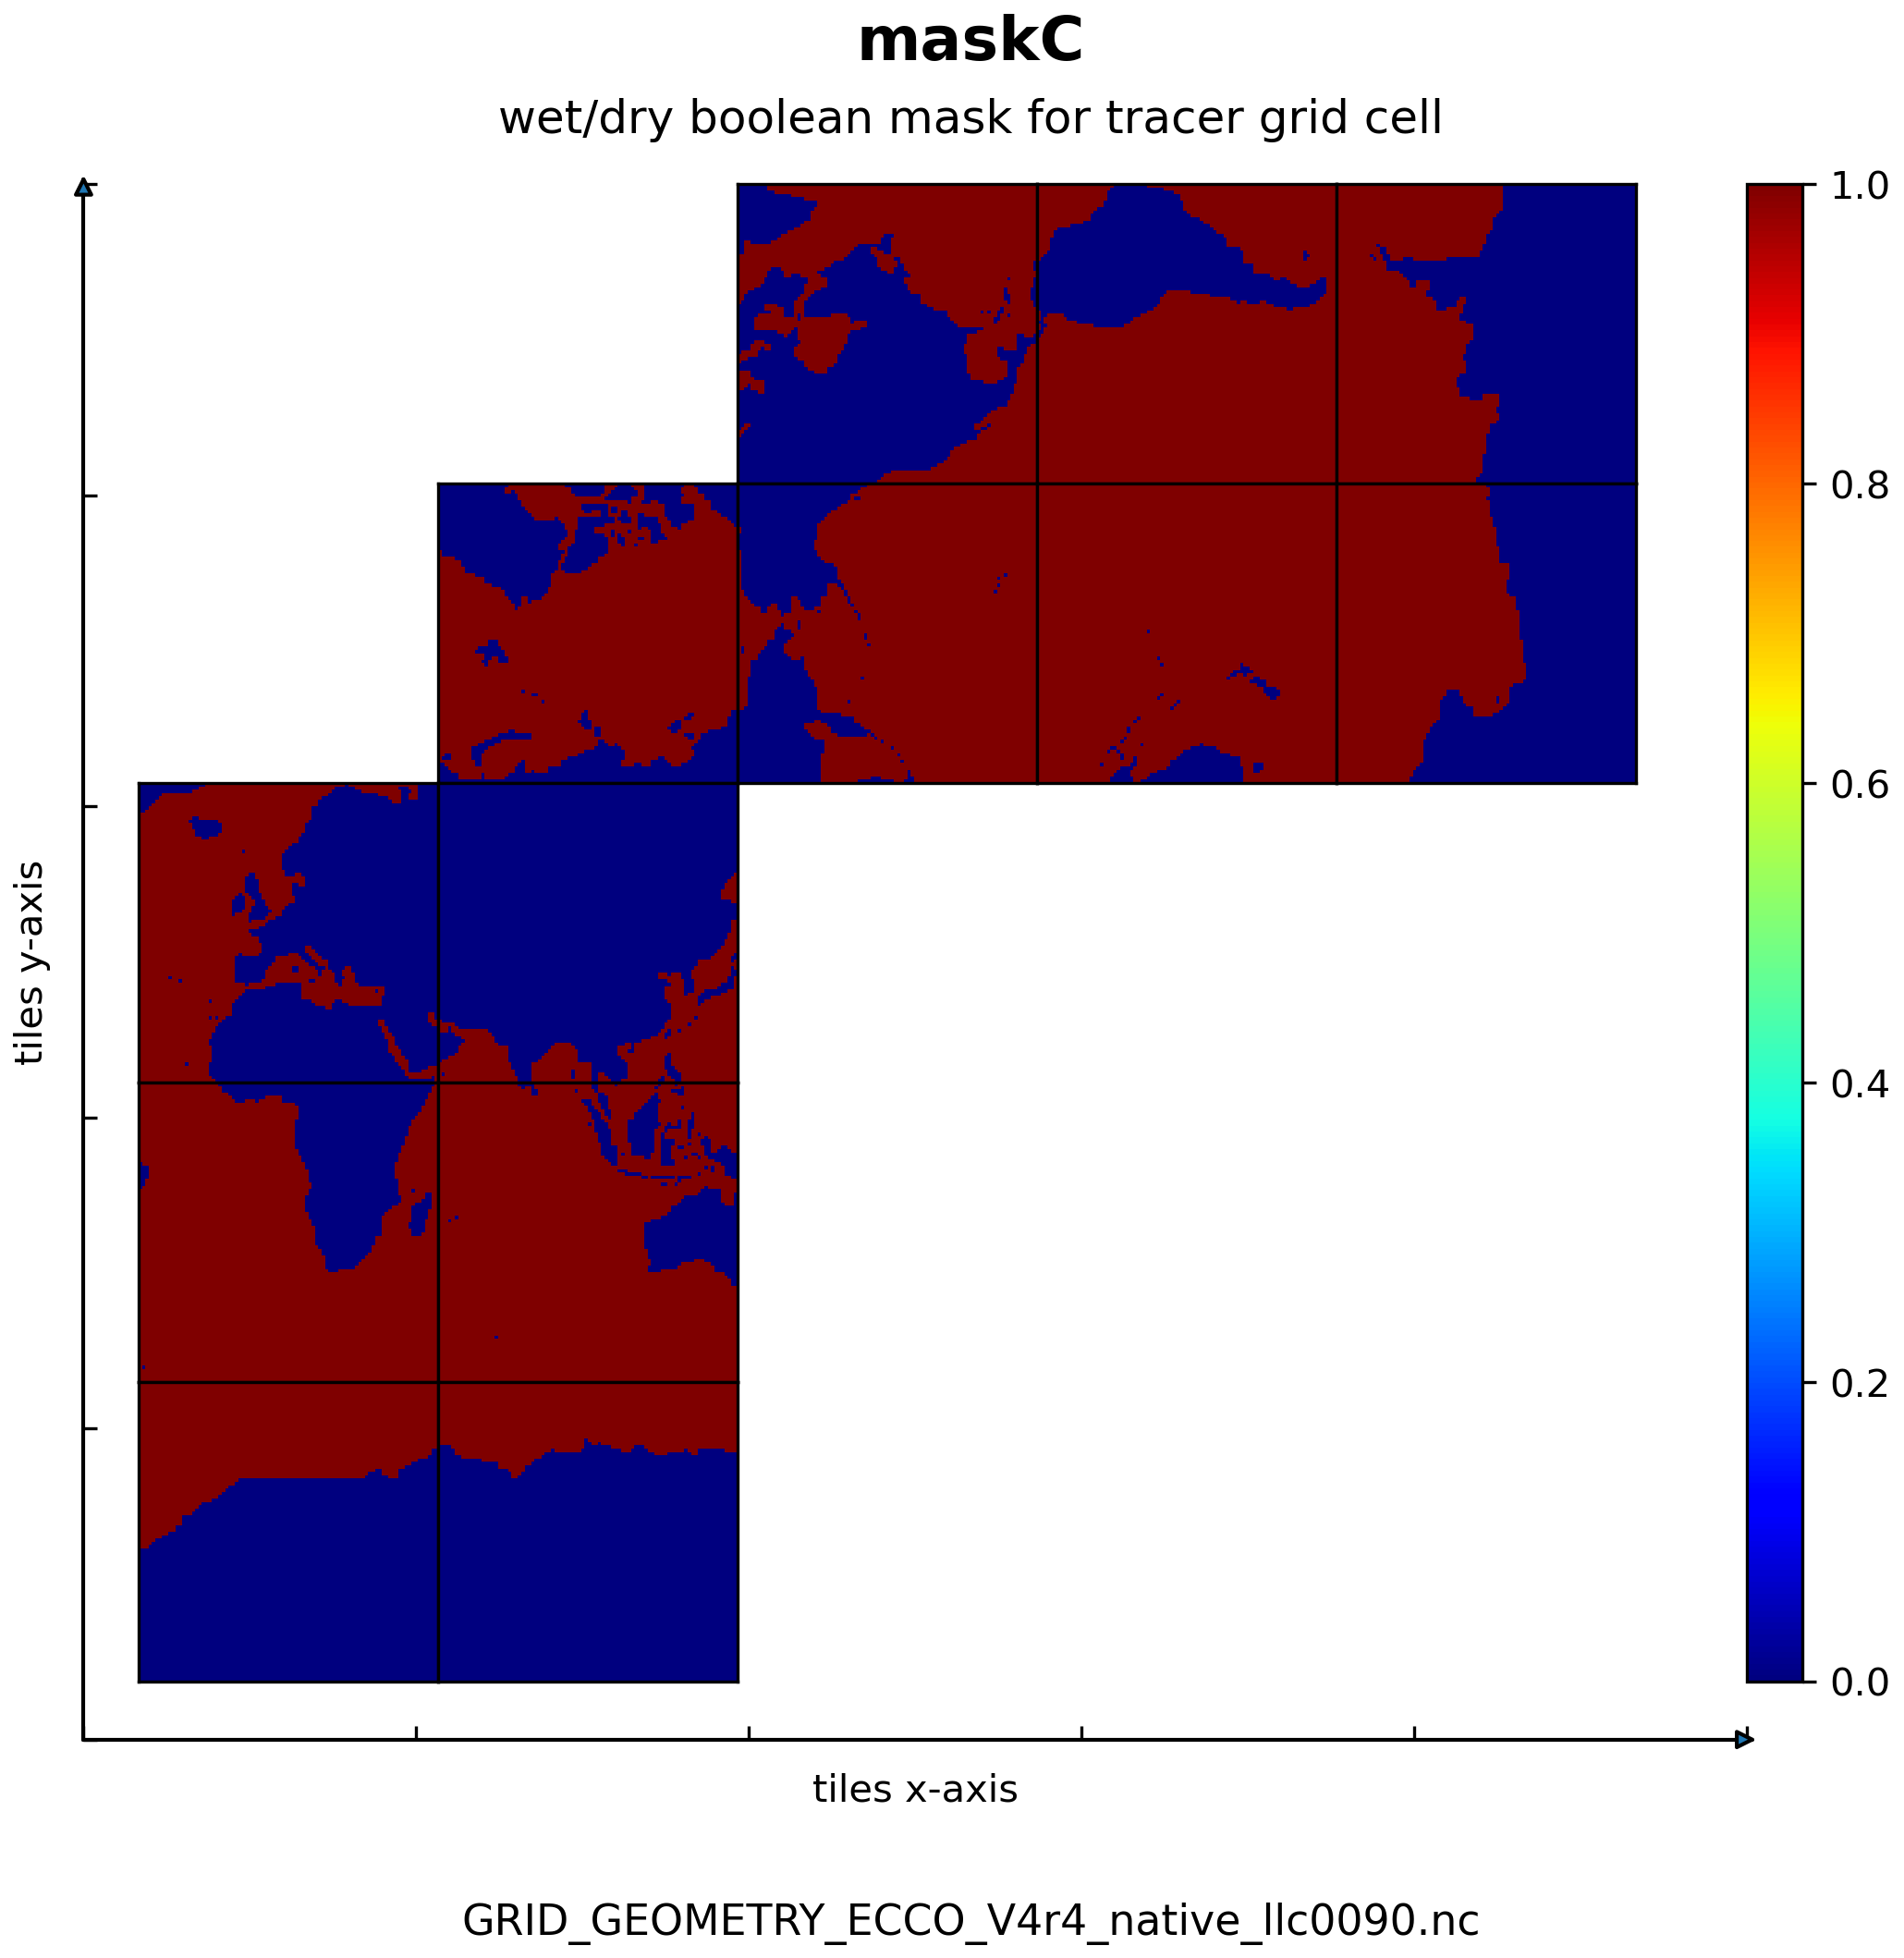
\includegraphics[scale=0.55]{../images/plots/native_plots_coords/Geometry_Parameters_for_the_Lat-Lon-Cap_90_(llc90)_Native_Model_Grid_(Version_4_Release_4)/maskC.png}
\caption{Dataset: GRID\_GEOMETRY\_ECCO, Variable: maskC}
\label{tab:table-GRID_GEOMETRY_ECCO_maskC-Plot}
\end{figure}
\pagebreak
\subsubsection{Native coordinates Variable: maskW}
\begin{longtable}{|m{0.06\textwidth}|m{0.3\textwidth}|m{0.45\textwidth}|m{0.11\textwidth}|}
\caption{Attributes description of the variable 'maskW' from GRID\_GEOMETRY\_ECCO's  dataset.}
\label{tab:table-GRID_GEOMETRY_ECCO_maskW} \\ 
\hline \endhead \hline \endfoot
\rowcolor{lightgray} \textbf{Storage Type} & \textbf{Variable Name} & \textbf{Description} & \textbf{Unit} \\ \hline
bool & maskW & Wet/dry boolean mask for 'west' face of tracer grid cell & N/A \\ \hline
\multicolumn{4}{|c|}{\cellcolor{lightgray}{\textbf{Description of the variable in Common Data language (CDL)}}} \\ \hline
\multicolumn{4}{|c|}{\makecell{\parbox{.92\textwidth}{bool maskW(k, tile, j, i\_g)\\
\hspace*{0.5cm}maskW: \_FillValue = 1\\
\hspace*{0.5cm}maskW: long\_name = "wet/dry boolean mask for west face of tracer grid cell"\\
\hspace*{0.5cm}maskW: coverage\_content\_type = modelResult\\
\hspace*{0.5cm}maskW: coordinates = Z}}} \\ \hline
\rowcolor{lightgray} \multicolumn{4}{|c|}{\textbf{Comments}} \\ \hline
\multicolumn{4}{|p{1\textwidth}|}{True for grid cells with nonzero open vertical fraction along their 'west' face (hfacw > 0), otherwise false. although hfacw can vary though time, cells will never close if starting open and will never open if starting closed: hfacw(i,j,k,t) > 0 for all t, if hfacw(i,j,k,t=0) and hfacw(i,j,k,t) = 0 for all t, if hfacw(i,j,k,t=0) = 0. therefore, maskw is time invariant. note: } \\ \hline
\end{longtable}

\begin{figure}[H]
\centering
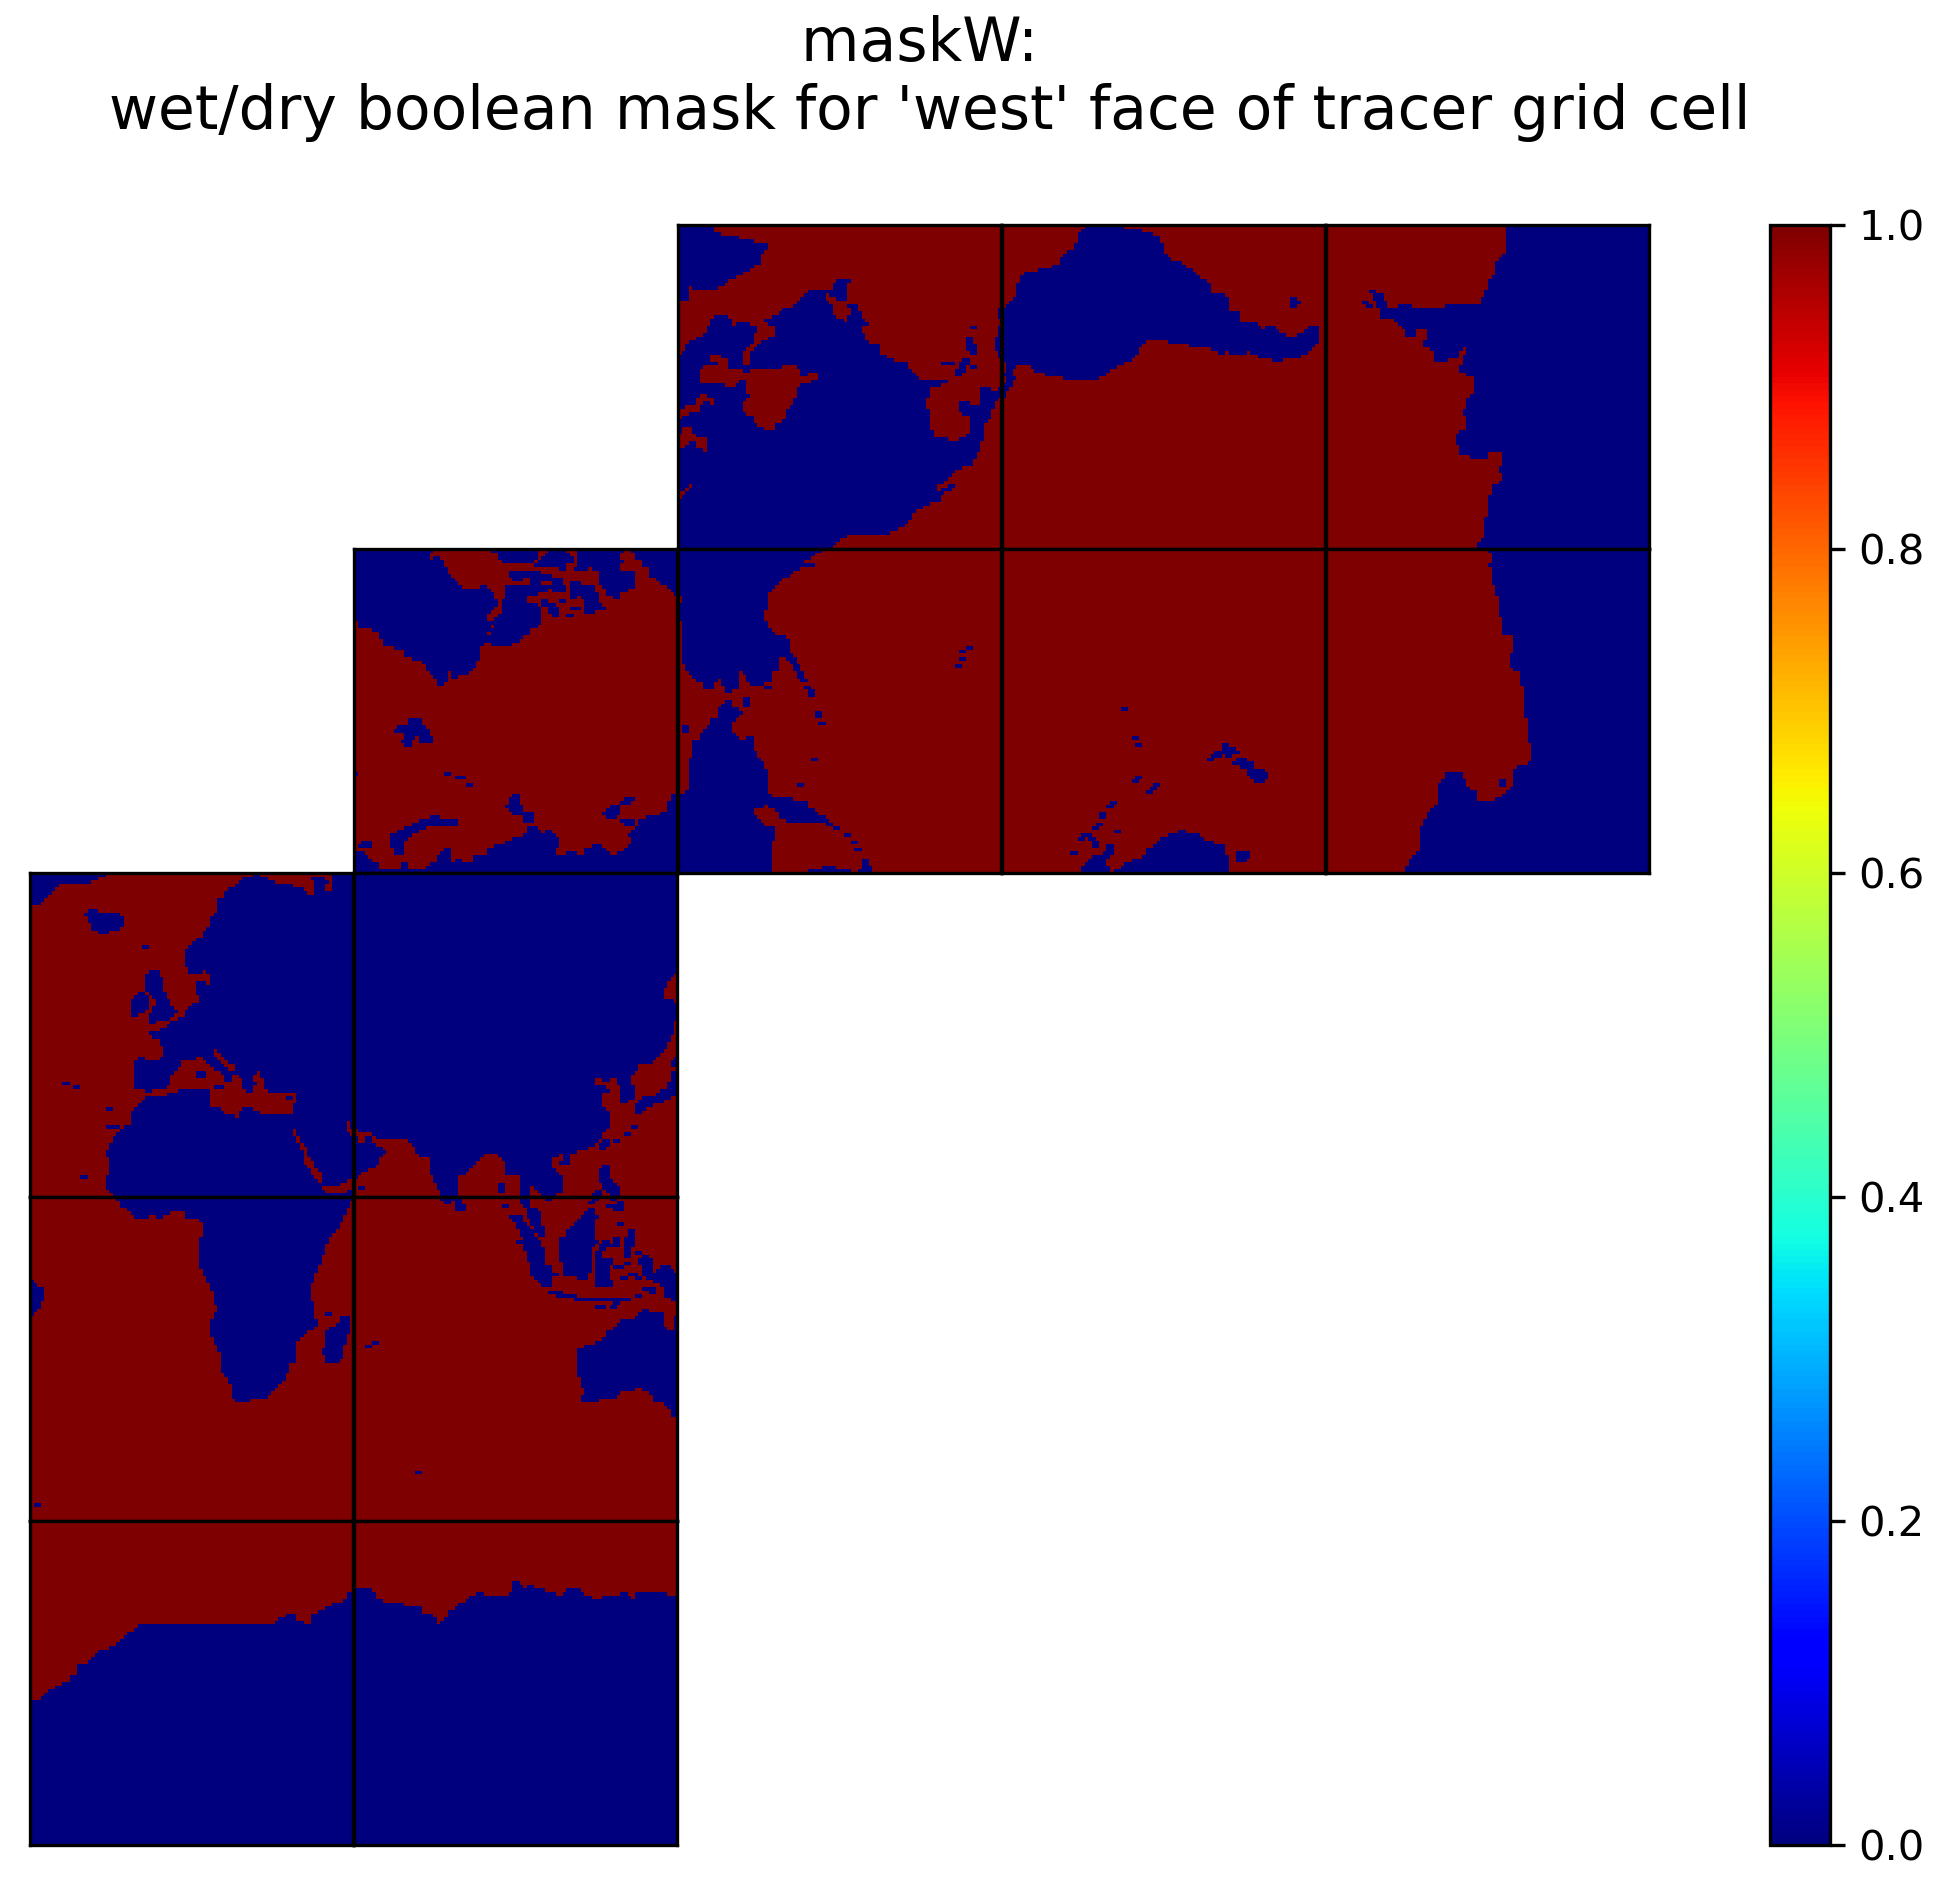
\includegraphics[scale=0.55]{../images/plots/native_plots_coords/Geometry_Parameters_for_the_Lat-Lon-Cap_90_(llc90)_Native_Model_Grid_(Version_4_Release_4)/maskW.png}
\caption{Dataset: GRID\_GEOMETRY\_ECCO, Variable: maskW}
\label{tab:table-GRID_GEOMETRY_ECCO_maskW-Plot}
\end{figure}
\pagebreak
\subsubsection{Native coordinates Variable: maskS}
\begin{longtable}{|m{0.06\textwidth}|m{0.3\textwidth}|m{0.45\textwidth}|m{0.11\textwidth}|}
\caption{Attributes description of the variable 'maskS' from GRID\_GEOMETRY\_ECCO's  dataset.}
\label{tab:table-GRID_GEOMETRY_ECCO_maskS} \\ 
\hline \endhead \hline \endfoot
\rowcolor{lightgray} \textbf{Storage Type} & \textbf{Variable Name} & \textbf{Description} & \textbf{Unit} \\ \hline
bool & maskS & Wet/dry boolean mask for 'south' face of tracer grid cell & N/A \\ \hline
\multicolumn{4}{|c|}{\cellcolor{lightgray}{\textbf{Description of the variable in Common Data language (CDL)}}} \\ \hline
\multicolumn{4}{|c|}{\makecell{\parbox{.92\textwidth}{bool maskS(k, tile, j\_g, i)\\
\hspace*{0.5cm}maskS: \_FillValue = 1\\
\hspace*{0.5cm}maskS: long\_name = "wet/dry boolean mask for south face of tracer grid cell"\\
\hspace*{0.5cm}maskS: coverage\_content\_type = modelResult\\
\hspace*{0.5cm}maskS: coordinates = Z}}} \\ \hline
\rowcolor{lightgray} \multicolumn{4}{|c|}{\textbf{Comments}} \\ \hline
\multicolumn{4}{|p{1\textwidth}|}{True for grid cells with nonzero open vertical fraction along their 'south' face (hfacs > 0), otherwise false. although hfacs can vary though time, cells will never close if starting open and will never open if starting closed: hfacs(i,j,k,t) > 0 for all t, if hfacs(i,j,k,t=0) and hfacs(i,j,k,t) = 0 for all t, if hfacs(i,j,k,t=0) = 0. therefore, masks is time invariant. note: } \\ \hline
\end{longtable}

\begin{figure}[H]
\centering
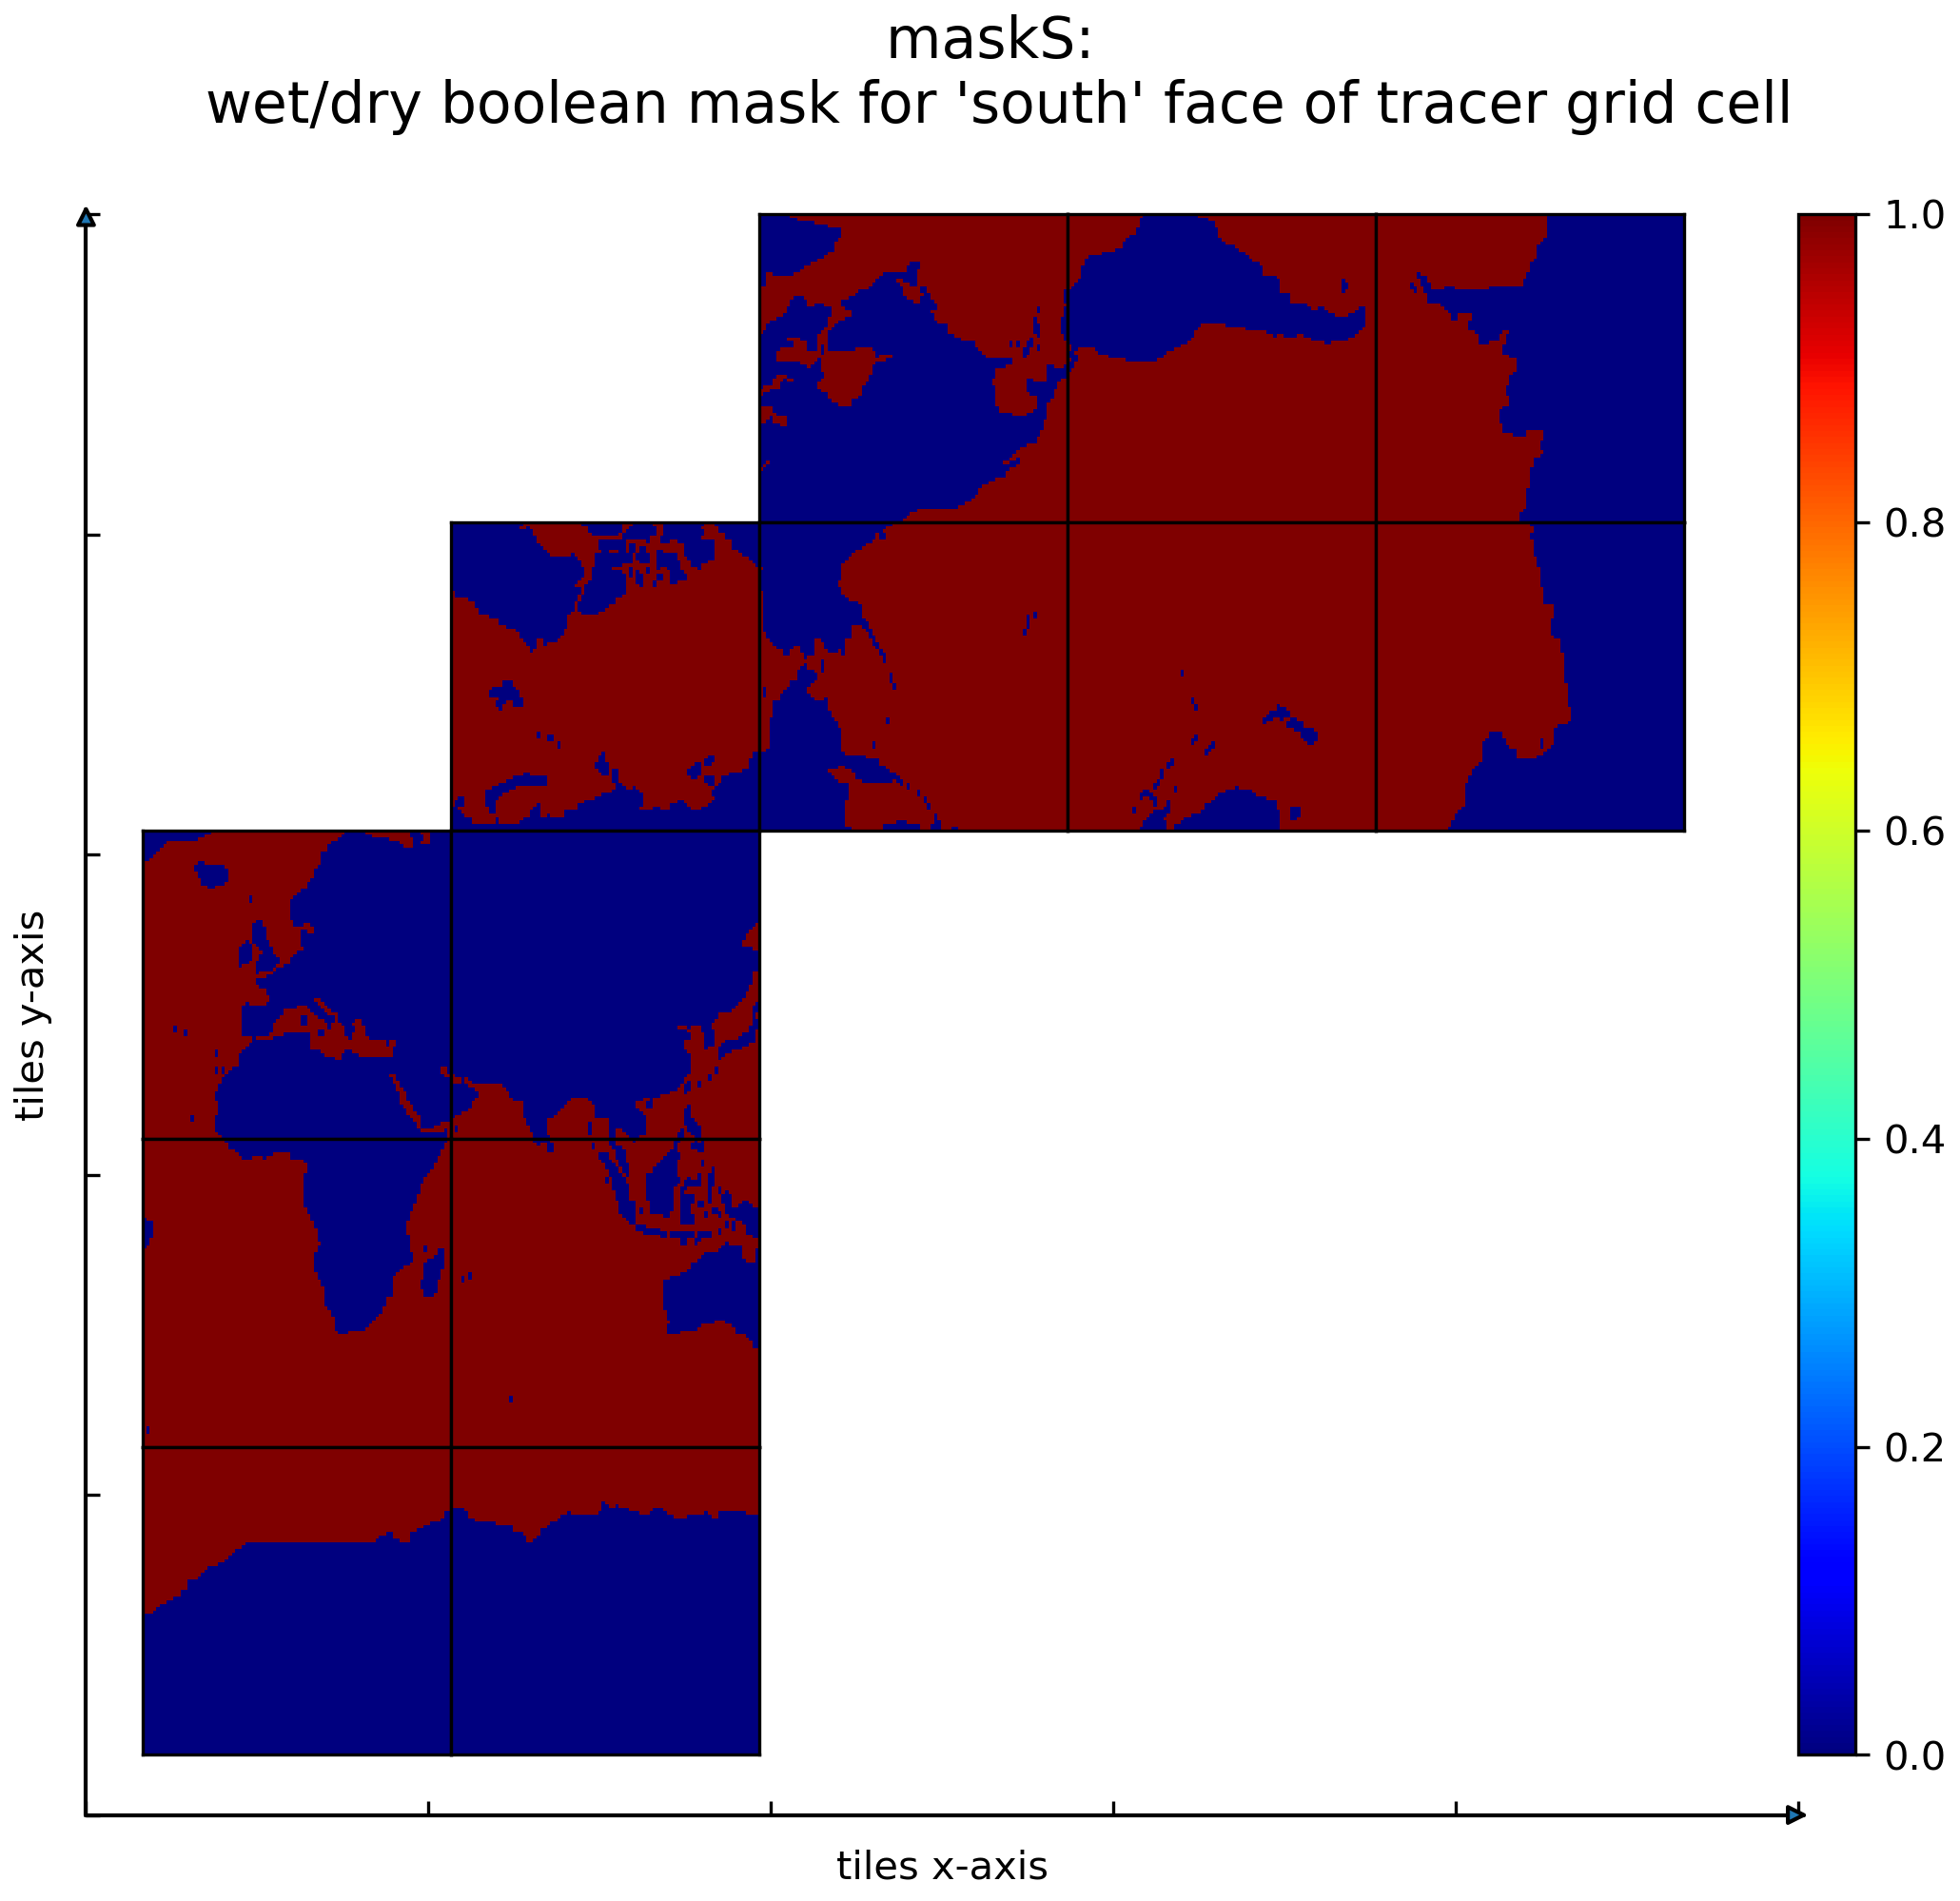
\includegraphics[scale=0.55]{../images/plots/native_plots_coords/Geometry_Parameters_for_the_Lat-Lon-Cap_90_(llc90)_Native_Model_Grid_(Version_4_Release_4)/maskS.png}
\caption{Dataset: GRID\_GEOMETRY\_ECCO, Variable: maskS}
\label{tab:table-GRID_GEOMETRY_ECCO_maskS-Plot}
\end{figure}